\documentclass{article}

% use numbers for citations to save space
\PassOptionsToPackage{numbers, compress}{natbib}

% either empty (for submission), 'preprint', or 'final'
\def\status{preprint}
\usepackage[\status]{neurips_2024}

% TOC for document parts, must be included before hyperref!
% (https://latex.org/forum/viewtopic.php?t=2014)
\usepackage{titletoc}
%%% Local Variables:
%%% mode: latex
%%% TeX-master: "../main"
%%% End:

\documentclass{article}


% if you need to pass options to natbib, use, e.g.:
%     \PassOptionsToPackage{numbers, compress}{natbib}
% before loading neurips_2024


% ready for submission
\usepackage{neurips_2024}


% to compile a preprint version, e.g., for submission to arXiv, add add the
% [preprint] option:
%     \usepackage[preprint]{neurips_2024}


% to compile a camera-ready version, add the [final] option, e.g.:
%     \usepackage[final]{neurips_2024}


% to avoid loading the natbib package, add option nonatbib:
%    \usepackage[nonatbib]{neurips_2024}


\usepackage[utf8]{inputenc} % allow utf-8 input
\usepackage[T1]{fontenc}    % use 8-bit T1 fonts
\usepackage{hyperref}       % hyperlinks
\usepackage{url}            % simple URL typesetting
\usepackage{booktabs}       % professional-quality tables
\usepackage{amsfonts}       % blackboard math symbols
\usepackage{nicefrac}       % compact symbols for 1/2, etc.
\usepackage{microtype}      % microtypography
\usepackage{xcolor}         % colors


\title{Formatting Instructions For NeurIPS 2024}


% The \author macro works with any number of authors. There are two commands
% used to separate the names and addresses of multiple authors: \And and \AND.
%
% Using \And between authors leaves it to LaTeX to determine where to break the
% lines. Using \AND forces a line break at that point. So, if LaTeX puts 3 of 4
% authors names on the first line, and the last on the second line, try using
% \AND instead of \And before the third author name.


\author{%
  David S.~Hippocampus\thanks{Use footnote for providing further information
    about author (webpage, alternative address)---\emph{not} for acknowledging
    funding agencies.} \\
  Department of Computer Science\\
  Cranberry-Lemon University\\
  Pittsburgh, PA 15213 \\
  \texttt{hippo@cs.cranberry-lemon.edu} \\
  % examples of more authors
  % \And
  % Coauthor \\
  % Affiliation \\
  % Address \\
  % \texttt{email} \\
  % \AND
  % Coauthor \\
  % Affiliation \\
  % Address \\
  % \texttt{email} \\
  % \And
  % Coauthor \\
  % Affiliation \\
  % Address \\
  % \texttt{email} \\
  % \And
  % Coauthor \\
  % Affiliation \\
  % Address \\
  % \texttt{email} \\
}


\begin{document}


\maketitle


\begin{abstract}
  The abstract paragraph should be indented \nicefrac{1}{2}~inch (3~picas) on
  both the left- and right-hand margins. Use 10~point type, with a vertical
  spacing (leading) of 11~points.  The word \textbf{Abstract} must be centered,
  bold, and in point size 12. Two line spaces precede the abstract. The abstract
  must be limited to one paragraph.
\end{abstract}


\section{Submission of papers to NeurIPS 2024}


Please read the instructions below carefully and follow them faithfully.


\subsection{Style}


Papers to be submitted to NeurIPS 2024 must be prepared according to the
instructions presented here. Papers may only be up to {\bf nine} pages long,
including figures. Additional pages \emph{containing only acknowledgments and
references} are allowed. Papers that exceed the page limit will not be
reviewed, or in any other way considered for presentation at the conference.


The margins in 2024 are the same as those in previous years.


Authors are required to use the NeurIPS \LaTeX{} style files obtainable at the
NeurIPS website as indicated below. Please make sure you use the current files
and not previous versions. Tweaking the style files may be grounds for
rejection.


\subsection{Retrieval of style files}


The style files for NeurIPS and other conference information are available on
the website at
\begin{center}
  \url{http://www.neurips.cc/}
\end{center}
The file \verb+neurips_2024.pdf+ contains these instructions and illustrates the
various formatting requirements your NeurIPS paper must satisfy.


The only supported style file for NeurIPS 2024 is \verb+neurips_2024.sty+,
rewritten for \LaTeXe{}.  \textbf{Previous style files for \LaTeX{} 2.09,
  Microsoft Word, and RTF are no longer supported!}


The \LaTeX{} style file contains three optional arguments: \verb+final+, which
creates a camera-ready copy, \verb+preprint+, which creates a preprint for
submission to, e.g., arXiv, and \verb+nonatbib+, which will not load the
\verb+natbib+ package for you in case of package clash.


\paragraph{Preprint option}
If you wish to post a preprint of your work online, e.g., on arXiv, using the
NeurIPS style, please use the \verb+preprint+ option. This will create a
nonanonymized version of your work with the text ``Preprint. Work in progress.''
in the footer. This version may be distributed as you see fit, as long as you do not say which conference it was submitted to. Please \textbf{do
  not} use the \verb+final+ option, which should \textbf{only} be used for
papers accepted to NeurIPS.


At submission time, please omit the \verb+final+ and \verb+preprint+
options. This will anonymize your submission and add line numbers to aid
review. Please do \emph{not} refer to these line numbers in your paper as they
will be removed during generation of camera-ready copies.


The file \verb+neurips_2024.tex+ may be used as a ``shell'' for writing your
paper. All you have to do is replace the author, title, abstract, and text of
the paper with your own.


The formatting instructions contained in these style files are summarized in
Sections \ref{gen_inst}, \ref{headings}, and \ref{others} below.


\section{General formatting instructions}
\label{gen_inst}


The text must be confined within a rectangle 5.5~inches (33~picas) wide and
9~inches (54~picas) long. The left margin is 1.5~inch (9~picas).  Use 10~point
type with a vertical spacing (leading) of 11~points.  Times New Roman is the
preferred typeface throughout, and will be selected for you by default.
Paragraphs are separated by \nicefrac{1}{2}~line space (5.5 points), with no
indentation.


The paper title should be 17~point, initial caps/lower case, bold, centered
between two horizontal rules. The top rule should be 4~points thick and the
bottom rule should be 1~point thick. Allow \nicefrac{1}{4}~inch space above and
below the title to rules. All pages should start at 1~inch (6~picas) from the
top of the page.


For the final version, authors' names are set in boldface, and each name is
centered above the corresponding address. The lead author's name is to be listed
first (left-most), and the co-authors' names (if different address) are set to
follow. If there is only one co-author, list both author and co-author side by
side.


Please pay special attention to the instructions in Section \ref{others}
regarding figures, tables, acknowledgments, and references.


\section{Headings: first level}
\label{headings}


All headings should be lower case (except for first word and proper nouns),
flush left, and bold.


First-level headings should be in 12-point type.


\subsection{Headings: second level}


Second-level headings should be in 10-point type.


\subsubsection{Headings: third level}


Third-level headings should be in 10-point type.


\paragraph{Paragraphs}


There is also a \verb+\paragraph+ command available, which sets the heading in
bold, flush left, and inline with the text, with the heading followed by 1\,em
of space.


\section{Citations, figures, tables, references}
\label{others}


These instructions apply to everyone.


\subsection{Citations within the text}


The \verb+natbib+ package will be loaded for you by default.  Citations may be
author/year or numeric, as long as you maintain internal consistency.  As to the
format of the references themselves, any style is acceptable as long as it is
used consistently.


The documentation for \verb+natbib+ may be found at
\begin{center}
  \url{http://mirrors.ctan.org/macros/latex/contrib/natbib/natnotes.pdf}
\end{center}
Of note is the command \verb+\citet+, which produces citations appropriate for
use in inline text.  For example,
\begin{verbatim}
   \citet{hasselmo} investigated\dots
\end{verbatim}
produces
\begin{quote}
  Hasselmo, et al.\ (1995) investigated\dots
\end{quote}


If you wish to load the \verb+natbib+ package with options, you may add the
following before loading the \verb+neurips_2024+ package:
\begin{verbatim}
   \PassOptionsToPackage{options}{natbib}
\end{verbatim}


If \verb+natbib+ clashes with another package you load, you can add the optional
argument \verb+nonatbib+ when loading the style file:
\begin{verbatim}
   \usepackage[nonatbib]{neurips_2024}
\end{verbatim}


As submission is double blind, refer to your own published work in the third
person. That is, use ``In the previous work of Jones et al.\ [4],'' not ``In our
previous work [4].'' If you cite your other papers that are not widely available
(e.g., a journal paper under review), use anonymous author names in the
citation, e.g., an author of the form ``A.\ Anonymous'' and include a copy of the anonymized paper in the supplementary material.


\subsection{Footnotes}


Footnotes should be used sparingly.  If you do require a footnote, indicate
footnotes with a number\footnote{Sample of the first footnote.} in the
text. Place the footnotes at the bottom of the page on which they appear.
Precede the footnote with a horizontal rule of 2~inches (12~picas).


Note that footnotes are properly typeset \emph{after} punctuation
marks.\footnote{As in this example.}


\subsection{Figures}


\begin{figure}
  \centering
  \fbox{\rule[-.5cm]{0cm}{4cm} \rule[-.5cm]{4cm}{0cm}}
  \caption{Sample figure caption.}
\end{figure}


All artwork must be neat, clean, and legible. Lines should be dark enough for
purposes of reproduction. The figure number and caption always appear after the
figure. Place one line space before the figure caption and one line space after
the figure. The figure caption should be lower case (except for first word and
proper nouns); figures are numbered consecutively.


You may use color figures.  However, it is best for the figure captions and the
paper body to be legible if the paper is printed in either black/white or in
color.


\subsection{Tables}


All tables must be centered, neat, clean and legible.  The table number and
title always appear before the table.  See Table~\ref{sample-table}.


Place one line space before the table title, one line space after the
table title, and one line space after the table. The table title must
be lower case (except for first word and proper nouns); tables are
numbered consecutively.


Note that publication-quality tables \emph{do not contain vertical rules.} We
strongly suggest the use of the \verb+booktabs+ package, which allows for
typesetting high-quality, professional tables:
\begin{center}
  \url{https://www.ctan.org/pkg/booktabs}
\end{center}
This package was used to typeset Table~\ref{sample-table}.


\begin{table}
  \caption{Sample table title}
  \label{sample-table}
  \centering
  \begin{tabular}{lll}
    \toprule
    \multicolumn{2}{c}{Part}                   \\
    \cmidrule(r){1-2}
    Name     & Description     & Size ($\mu$m) \\
    \midrule
    Dendrite & Input terminal  & $\sim$100     \\
    Axon     & Output terminal & $\sim$10      \\
    Soma     & Cell body       & up to $10^6$  \\
    \bottomrule
  \end{tabular}
\end{table}

\subsection{Math}
Note that display math in bare TeX commands will not create correct line numbers for submission. Please use LaTeX (or AMSTeX) commands for unnumbered display math. (You really shouldn't be using \$\$ anyway; see \url{https://tex.stackexchange.com/questions/503/why-is-preferable-to} and \url{https://tex.stackexchange.com/questions/40492/what-are-the-differences-between-align-equation-and-displaymath} for more information.)

\subsection{Final instructions}

Do not change any aspects of the formatting parameters in the style files.  In
particular, do not modify the width or length of the rectangle the text should
fit into, and do not change font sizes (except perhaps in the
\textbf{References} section; see below). Please note that pages should be
numbered.


\section{Preparing PDF files}


Please prepare submission files with paper size ``US Letter,'' and not, for
example, ``A4.''


Fonts were the main cause of problems in the past years. Your PDF file must only
contain Type 1 or Embedded TrueType fonts. Here are a few instructions to
achieve this.


\begin{itemize}


\item You should directly generate PDF files using \verb+pdflatex+.


\item You can check which fonts a PDF files uses.  In Acrobat Reader, select the
  menu Files$>$Document Properties$>$Fonts and select Show All Fonts. You can
  also use the program \verb+pdffonts+ which comes with \verb+xpdf+ and is
  available out-of-the-box on most Linux machines.


\item \verb+xfig+ "patterned" shapes are implemented with bitmap fonts.  Use
  "solid" shapes instead.


\item The \verb+\bbold+ package almost always uses bitmap fonts.  You should use
  the equivalent AMS Fonts:
\begin{verbatim}
   \usepackage{amsfonts}
\end{verbatim}
followed by, e.g., \verb+\mathbb{R}+, \verb+\mathbb{N}+, or \verb+\mathbb{C}+
for $\mathbb{R}$, $\mathbb{N}$ or $\mathbb{C}$.  You can also use the following
workaround for reals, natural and complex:
\begin{verbatim}
   \newcommand{\RR}{I\!\!R} %real numbers
   \newcommand{\Nat}{I\!\!N} %natural numbers
   \newcommand{\CC}{I\!\!\!\!C} %complex numbers
\end{verbatim}
Note that \verb+amsfonts+ is automatically loaded by the \verb+amssymb+ package.


\end{itemize}


If your file contains type 3 fonts or non embedded TrueType fonts, we will ask
you to fix it.


\subsection{Margins in \LaTeX{}}


Most of the margin problems come from figures positioned by hand using
\verb+\special+ or other commands. We suggest using the command
\verb+\includegraphics+ from the \verb+graphicx+ package. Always specify the
figure width as a multiple of the line width as in the example below:
\begin{verbatim}
   \usepackage[pdftex]{graphicx} ...
   \includegraphics[width=0.8\linewidth]{myfile.pdf}
\end{verbatim}
See Section 4.4 in the graphics bundle documentation
(\url{http://mirrors.ctan.org/macros/latex/required/graphics/grfguide.pdf})


A number of width problems arise when \LaTeX{} cannot properly hyphenate a
line. Please give LaTeX hyphenation hints using the \verb+\-+ command when
necessary.

\begin{ack}
Use unnumbered first level headings for the acknowledgments. All acknowledgments
go at the end of the paper before the list of references. Moreover, you are required to declare
funding (financial activities supporting the submitted work) and competing interests (related financial activities outside the submitted work).
More information about this disclosure can be found at: \url{https://neurips.cc/Conferences/2024/PaperInformation/FundingDisclosure}.


Do {\bf not} include this section in the anonymized submission, only in the final paper. You can use the \texttt{ack} environment provided in the style file to automatically hide this section in the anonymized submission.
\end{ack}

\section*{References}


References follow the acknowledgments in the camera-ready paper. Use unnumbered first-level heading for
the references. Any choice of citation style is acceptable as long as you are
consistent. It is permissible to reduce the font size to \verb+small+ (9 point)
when listing the references.
Note that the Reference section does not count towards the page limit.
\medskip


{
\small


[1] Alexander, J.A.\ \& Mozer, M.C.\ (1995) Template-based algorithms for
connectionist rule extraction. In G.\ Tesauro, D.S.\ Touretzky and T.K.\ Leen
(eds.), {\it Advances in Neural Information Processing Systems 7},
pp.\ 609--616. Cambridge, MA: MIT Press.


[2] Bower, J.M.\ \& Beeman, D.\ (1995) {\it The Book of GENESIS: Exploring
  Realistic Neural Models with the GEneral NEural SImulation System.}  New York:
TELOS/Springer--Verlag.


[3] Hasselmo, M.E., Schnell, E.\ \& Barkai, E.\ (1995) Dynamics of learning and
recall at excitatory recurrent synapses and cholinergic modulation in rat
hippocampal region CA3. {\it Journal of Neuroscience} {\bf 15}(7):5249-5262.
}


%%%%%%%%%%%%%%%%%%%%%%%%%%%%%%%%%%%%%%%%%%%%%%%%%%%%%%%%%%%%

\appendix

\section{Appendix / supplemental material}


Optionally include supplemental material (complete proofs, additional experiments and plots) in appendix.
All such materials \textbf{SHOULD be included in the main submission.}

%%%%%%%%%%%%%%%%%%%%%%%%%%%%%%%%%%%%%%%%%%%%%%%%%%%%%%%%%%%%

\newpage
\section*{NeurIPS Paper Checklist}

%%% BEGIN INSTRUCTIONS %%%
The checklist is designed to encourage best practices for responsible machine learning research, addressing issues of reproducibility, transparency, research ethics, and societal impact. Do not remove the checklist: {\bf The papers not including the checklist will be desk rejected.} The checklist should follow the references and follow the (optional) supplemental material.  The checklist does NOT count towards the page
limit. 

Please read the checklist guidelines carefully for information on how to answer these questions. For each question in the checklist:
\begin{itemize}
    \item You should answer \answerYes{}, \answerNo{}, or \answerNA{}.
    \item \answerNA{} means either that the question is Not Applicable for that particular paper or the relevant information is Not Available.
    \item Please provide a short (1–2 sentence) justification right after your answer (even for NA). 
   % \item {\bf The papers not including the checklist will be desk rejected.}
\end{itemize}

{\bf The checklist answers are an integral part of your paper submission.} They are visible to the reviewers, area chairs, senior area chairs, and ethics reviewers. You will be asked to also include it (after eventual revisions) with the final version of your paper, and its final version will be published with the paper.

The reviewers of your paper will be asked to use the checklist as one of the factors in their evaluation. While "\answerYes{}" is generally preferable to "\answerNo{}", it is perfectly acceptable to answer "\answerNo{}" provided a proper justification is given (e.g., "error bars are not reported because it would be too computationally expensive" or "we were unable to find the license for the dataset we used"). In general, answering "\answerNo{}" or "\answerNA{}" is not grounds for rejection. While the questions are phrased in a binary way, we acknowledge that the true answer is often more nuanced, so please just use your best judgment and write a justification to elaborate. All supporting evidence can appear either in the main paper or the supplemental material, provided in appendix. If you answer \answerYes{} to a question, in the justification please point to the section(s) where related material for the question can be found.

IMPORTANT, please:
\begin{itemize}
    \item {\bf Delete this instruction block, but keep the section heading ``NeurIPS paper checklist"},
    \item  {\bf Keep the checklist subsection headings, questions/answers and guidelines below.}
    \item {\bf Do not modify the questions and only use the provided macros for your answers}.
\end{itemize} 
 

%%% END INSTRUCTIONS %%%


\begin{enumerate}

\item {\bf Claims}
    \item[] Question: Do the main claims made in the abstract and introduction accurately reflect the paper's contributions and scope?
    \item[] Answer: \answerTODO{} % Replace by \answerYes{}, \answerNo{}, or \answerNA{}.
    \item[] Justification: \justificationTODO{}
    \item[] Guidelines:
    \begin{itemize}
        \item The answer NA means that the abstract and introduction do not include the claims made in the paper.
        \item The abstract and/or introduction should clearly state the claims made, including the contributions made in the paper and important assumptions and limitations. A No or NA answer to this question will not be perceived well by the reviewers. 
        \item The claims made should match theoretical and experimental results, and reflect how much the results can be expected to generalize to other settings. 
        \item It is fine to include aspirational goals as motivation as long as it is clear that these goals are not attained by the paper. 
    \end{itemize}

\item {\bf Limitations}
    \item[] Question: Does the paper discuss the limitations of the work performed by the authors?
    \item[] Answer: \answerTODO{} % Replace by \answerYes{}, \answerNo{}, or \answerNA{}.
    \item[] Justification: \justificationTODO{}
    \item[] Guidelines:
    \begin{itemize}
        \item The answer NA means that the paper has no limitation while the answer No means that the paper has limitations, but those are not discussed in the paper. 
        \item The authors are encouraged to create a separate "Limitations" section in their paper.
        \item The paper should point out any strong assumptions and how robust the results are to violations of these assumptions (e.g., independence assumptions, noiseless settings, model well-specification, asymptotic approximations only holding locally). The authors should reflect on how these assumptions might be violated in practice and what the implications would be.
        \item The authors should reflect on the scope of the claims made, e.g., if the approach was only tested on a few datasets or with a few runs. In general, empirical results often depend on implicit assumptions, which should be articulated.
        \item The authors should reflect on the factors that influence the performance of the approach. For example, a facial recognition algorithm may perform poorly when image resolution is low or images are taken in low lighting. Or a speech-to-text system might not be used reliably to provide closed captions for online lectures because it fails to handle technical jargon.
        \item The authors should discuss the computational efficiency of the proposed algorithms and how they scale with dataset size.
        \item If applicable, the authors should discuss possible limitations of their approach to address problems of privacy and fairness.
        \item While the authors might fear that complete honesty about limitations might be used by reviewers as grounds for rejection, a worse outcome might be that reviewers discover limitations that aren't acknowledged in the paper. The authors should use their best judgment and recognize that individual actions in favor of transparency play an important role in developing norms that preserve the integrity of the community. Reviewers will be specifically instructed to not penalize honesty concerning limitations.
    \end{itemize}

\item {\bf Theory Assumptions and Proofs}
    \item[] Question: For each theoretical result, does the paper provide the full set of assumptions and a complete (and correct) proof?
    \item[] Answer: \answerTODO{} % Replace by \answerYes{}, \answerNo{}, or \answerNA{}.
    \item[] Justification: \justificationTODO{}
    \item[] Guidelines:
    \begin{itemize}
        \item The answer NA means that the paper does not include theoretical results. 
        \item All the theorems, formulas, and proofs in the paper should be numbered and cross-referenced.
        \item All assumptions should be clearly stated or referenced in the statement of any theorems.
        \item The proofs can either appear in the main paper or the supplemental material, but if they appear in the supplemental material, the authors are encouraged to provide a short proof sketch to provide intuition. 
        \item Inversely, any informal proof provided in the core of the paper should be complemented by formal proofs provided in appendix or supplemental material.
        \item Theorems and Lemmas that the proof relies upon should be properly referenced. 
    \end{itemize}

    \item {\bf Experimental Result Reproducibility}
    \item[] Question: Does the paper fully disclose all the information needed to reproduce the main experimental results of the paper to the extent that it affects the main claims and/or conclusions of the paper (regardless of whether the code and data are provided or not)?
    \item[] Answer: \answerTODO{} % Replace by \answerYes{}, \answerNo{}, or \answerNA{}.
    \item[] Justification: \justificationTODO{}
    \item[] Guidelines:
    \begin{itemize}
        \item The answer NA means that the paper does not include experiments.
        \item If the paper includes experiments, a No answer to this question will not be perceived well by the reviewers: Making the paper reproducible is important, regardless of whether the code and data are provided or not.
        \item If the contribution is a dataset and/or model, the authors should describe the steps taken to make their results reproducible or verifiable. 
        \item Depending on the contribution, reproducibility can be accomplished in various ways. For example, if the contribution is a novel architecture, describing the architecture fully might suffice, or if the contribution is a specific model and empirical evaluation, it may be necessary to either make it possible for others to replicate the model with the same dataset, or provide access to the model. In general. releasing code and data is often one good way to accomplish this, but reproducibility can also be provided via detailed instructions for how to replicate the results, access to a hosted model (e.g., in the case of a large language model), releasing of a model checkpoint, or other means that are appropriate to the research performed.
        \item While NeurIPS does not require releasing code, the conference does require all submissions to provide some reasonable avenue for reproducibility, which may depend on the nature of the contribution. For example
        \begin{enumerate}
            \item If the contribution is primarily a new algorithm, the paper should make it clear how to reproduce that algorithm.
            \item If the contribution is primarily a new model architecture, the paper should describe the architecture clearly and fully.
            \item If the contribution is a new model (e.g., a large language model), then there should either be a way to access this model for reproducing the results or a way to reproduce the model (e.g., with an open-source dataset or instructions for how to construct the dataset).
            \item We recognize that reproducibility may be tricky in some cases, in which case authors are welcome to describe the particular way they provide for reproducibility. In the case of closed-source models, it may be that access to the model is limited in some way (e.g., to registered users), but it should be possible for other researchers to have some path to reproducing or verifying the results.
        \end{enumerate}
    \end{itemize}


\item {\bf Open access to data and code}
    \item[] Question: Does the paper provide open access to the data and code, with sufficient instructions to faithfully reproduce the main experimental results, as described in supplemental material?
    \item[] Answer: \answerTODO{} % Replace by \answerYes{}, \answerNo{}, or \answerNA{}.
    \item[] Justification: \justificationTODO{}
    \item[] Guidelines:
    \begin{itemize}
        \item The answer NA means that paper does not include experiments requiring code.
        \item Please see the NeurIPS code and data submission guidelines (\url{https://nips.cc/public/guides/CodeSubmissionPolicy}) for more details.
        \item While we encourage the release of code and data, we understand that this might not be possible, so “No” is an acceptable answer. Papers cannot be rejected simply for not including code, unless this is central to the contribution (e.g., for a new open-source benchmark).
        \item The instructions should contain the exact command and environment needed to run to reproduce the results. See the NeurIPS code and data submission guidelines (\url{https://nips.cc/public/guides/CodeSubmissionPolicy}) for more details.
        \item The authors should provide instructions on data access and preparation, including how to access the raw data, preprocessed data, intermediate data, and generated data, etc.
        \item The authors should provide scripts to reproduce all experimental results for the new proposed method and baselines. If only a subset of experiments are reproducible, they should state which ones are omitted from the script and why.
        \item At submission time, to preserve anonymity, the authors should release anonymized versions (if applicable).
        \item Providing as much information as possible in supplemental material (appended to the paper) is recommended, but including URLs to data and code is permitted.
    \end{itemize}


\item {\bf Experimental Setting/Details}
    \item[] Question: Does the paper specify all the training and test details (e.g., data splits, hyperparameters, how they were chosen, type of optimizer, etc.) necessary to understand the results?
    \item[] Answer: \answerTODO{} % Replace by \answerYes{}, \answerNo{}, or \answerNA{}.
    \item[] Justification: \justificationTODO{}
    \item[] Guidelines:
    \begin{itemize}
        \item The answer NA means that the paper does not include experiments.
        \item The experimental setting should be presented in the core of the paper to a level of detail that is necessary to appreciate the results and make sense of them.
        \item The full details can be provided either with the code, in appendix, or as supplemental material.
    \end{itemize}

\item {\bf Experiment Statistical Significance}
    \item[] Question: Does the paper report error bars suitably and correctly defined or other appropriate information about the statistical significance of the experiments?
    \item[] Answer: \answerTODO{} % Replace by \answerYes{}, \answerNo{}, or \answerNA{}.
    \item[] Justification: \justificationTODO{}
    \item[] Guidelines:
    \begin{itemize}
        \item The answer NA means that the paper does not include experiments.
        \item The authors should answer "Yes" if the results are accompanied by error bars, confidence intervals, or statistical significance tests, at least for the experiments that support the main claims of the paper.
        \item The factors of variability that the error bars are capturing should be clearly stated (for example, train/test split, initialization, random drawing of some parameter, or overall run with given experimental conditions).
        \item The method for calculating the error bars should be explained (closed form formula, call to a library function, bootstrap, etc.)
        \item The assumptions made should be given (e.g., Normally distributed errors).
        \item It should be clear whether the error bar is the standard deviation or the standard error of the mean.
        \item It is OK to report 1-sigma error bars, but one should state it. The authors should preferably report a 2-sigma error bar than state that they have a 96\% CI, if the hypothesis of Normality of errors is not verified.
        \item For asymmetric distributions, the authors should be careful not to show in tables or figures symmetric error bars that would yield results that are out of range (e.g. negative error rates).
        \item If error bars are reported in tables or plots, The authors should explain in the text how they were calculated and reference the corresponding figures or tables in the text.
    \end{itemize}

\item {\bf Experiments Compute Resources}
    \item[] Question: For each experiment, does the paper provide sufficient information on the computer resources (type of compute workers, memory, time of execution) needed to reproduce the experiments?
    \item[] Answer: \answerTODO{} % Replace by \answerYes{}, \answerNo{}, or \answerNA{}.
    \item[] Justification: \justificationTODO{}
    \item[] Guidelines:
    \begin{itemize}
        \item The answer NA means that the paper does not include experiments.
        \item The paper should indicate the type of compute workers CPU or GPU, internal cluster, or cloud provider, including relevant memory and storage.
        \item The paper should provide the amount of compute required for each of the individual experimental runs as well as estimate the total compute. 
        \item The paper should disclose whether the full research project required more compute than the experiments reported in the paper (e.g., preliminary or failed experiments that didn't make it into the paper). 
    \end{itemize}
    
\item {\bf Code Of Ethics}
    \item[] Question: Does the research conducted in the paper conform, in every respect, with the NeurIPS Code of Ethics \url{https://neurips.cc/public/EthicsGuidelines}?
    \item[] Answer: \answerTODO{} % Replace by \answerYes{}, \answerNo{}, or \answerNA{}.
    \item[] Justification: \justificationTODO{}
    \item[] Guidelines:
    \begin{itemize}
        \item The answer NA means that the authors have not reviewed the NeurIPS Code of Ethics.
        \item If the authors answer No, they should explain the special circumstances that require a deviation from the Code of Ethics.
        \item The authors should make sure to preserve anonymity (e.g., if there is a special consideration due to laws or regulations in their jurisdiction).
    \end{itemize}


\item {\bf Broader Impacts}
    \item[] Question: Does the paper discuss both potential positive societal impacts and negative societal impacts of the work performed?
    \item[] Answer: \answerTODO{} % Replace by \answerYes{}, \answerNo{}, or \answerNA{}.
    \item[] Justification: \justificationTODO{}
    \item[] Guidelines:
    \begin{itemize}
        \item The answer NA means that there is no societal impact of the work performed.
        \item If the authors answer NA or No, they should explain why their work has no societal impact or why the paper does not address societal impact.
        \item Examples of negative societal impacts include potential malicious or unintended uses (e.g., disinformation, generating fake profiles, surveillance), fairness considerations (e.g., deployment of technologies that could make decisions that unfairly impact specific groups), privacy considerations, and security considerations.
        \item The conference expects that many papers will be foundational research and not tied to particular applications, let alone deployments. However, if there is a direct path to any negative applications, the authors should point it out. For example, it is legitimate to point out that an improvement in the quality of generative models could be used to generate deepfakes for disinformation. On the other hand, it is not needed to point out that a generic algorithm for optimizing neural networks could enable people to train models that generate Deepfakes faster.
        \item The authors should consider possible harms that could arise when the technology is being used as intended and functioning correctly, harms that could arise when the technology is being used as intended but gives incorrect results, and harms following from (intentional or unintentional) misuse of the technology.
        \item If there are negative societal impacts, the authors could also discuss possible mitigation strategies (e.g., gated release of models, providing defenses in addition to attacks, mechanisms for monitoring misuse, mechanisms to monitor how a system learns from feedback over time, improving the efficiency and accessibility of ML).
    \end{itemize}
    
\item {\bf Safeguards}
    \item[] Question: Does the paper describe safeguards that have been put in place for responsible release of data or models that have a high risk for misuse (e.g., pretrained language models, image generators, or scraped datasets)?
    \item[] Answer: \answerTODO{} % Replace by \answerYes{}, \answerNo{}, or \answerNA{}.
    \item[] Justification: \justificationTODO{}
    \item[] Guidelines:
    \begin{itemize}
        \item The answer NA means that the paper poses no such risks.
        \item Released models that have a high risk for misuse or dual-use should be released with necessary safeguards to allow for controlled use of the model, for example by requiring that users adhere to usage guidelines or restrictions to access the model or implementing safety filters. 
        \item Datasets that have been scraped from the Internet could pose safety risks. The authors should describe how they avoided releasing unsafe images.
        \item We recognize that providing effective safeguards is challenging, and many papers do not require this, but we encourage authors to take this into account and make a best faith effort.
    \end{itemize}

\item {\bf Licenses for existing assets}
    \item[] Question: Are the creators or original owners of assets (e.g., code, data, models), used in the paper, properly credited and are the license and terms of use explicitly mentioned and properly respected?
    \item[] Answer: \answerTODO{} % Replace by \answerYes{}, \answerNo{}, or \answerNA{}.
    \item[] Justification: \justificationTODO{}
    \item[] Guidelines:
    \begin{itemize}
        \item The answer NA means that the paper does not use existing assets.
        \item The authors should cite the original paper that produced the code package or dataset.
        \item The authors should state which version of the asset is used and, if possible, include a URL.
        \item The name of the license (e.g., CC-BY 4.0) should be included for each asset.
        \item For scraped data from a particular source (e.g., website), the copyright and terms of service of that source should be provided.
        \item If assets are released, the license, copyright information, and terms of use in the package should be provided. For popular datasets, \url{paperswithcode.com/datasets} has curated licenses for some datasets. Their licensing guide can help determine the license of a dataset.
        \item For existing datasets that are re-packaged, both the original license and the license of the derived asset (if it has changed) should be provided.
        \item If this information is not available online, the authors are encouraged to reach out to the asset's creators.
    \end{itemize}

\item {\bf New Assets}
    \item[] Question: Are new assets introduced in the paper well documented and is the documentation provided alongside the assets?
    \item[] Answer: \answerTODO{} % Replace by \answerYes{}, \answerNo{}, or \answerNA{}.
    \item[] Justification: \justificationTODO{}
    \item[] Guidelines:
    \begin{itemize}
        \item The answer NA means that the paper does not release new assets.
        \item Researchers should communicate the details of the dataset/code/model as part of their submissions via structured templates. This includes details about training, license, limitations, etc. 
        \item The paper should discuss whether and how consent was obtained from people whose asset is used.
        \item At submission time, remember to anonymize your assets (if applicable). You can either create an anonymized URL or include an anonymized zip file.
    \end{itemize}

\item {\bf Crowdsourcing and Research with Human Subjects}
    \item[] Question: For crowdsourcing experiments and research with human subjects, does the paper include the full text of instructions given to participants and screenshots, if applicable, as well as details about compensation (if any)? 
    \item[] Answer: \answerTODO{} % Replace by \answerYes{}, \answerNo{}, or \answerNA{}.
    \item[] Justification: \justificationTODO{}
    \item[] Guidelines:
    \begin{itemize}
        \item The answer NA means that the paper does not involve crowdsourcing nor research with human subjects.
        \item Including this information in the supplemental material is fine, but if the main contribution of the paper involves human subjects, then as much detail as possible should be included in the main paper. 
        \item According to the NeurIPS Code of Ethics, workers involved in data collection, curation, or other labor should be paid at least the minimum wage in the country of the data collector. 
    \end{itemize}

\item {\bf Institutional Review Board (IRB) Approvals or Equivalent for Research with Human Subjects}
    \item[] Question: Does the paper describe potential risks incurred by study participants, whether such risks were disclosed to the subjects, and whether Institutional Review Board (IRB) approvals (or an equivalent approval/review based on the requirements of your country or institution) were obtained?
    \item[] Answer: \answerTODO{} % Replace by \answerYes{}, \answerNo{}, or \answerNA{}.
    \item[] Justification: \justificationTODO{}
    \item[] Guidelines:
    \begin{itemize}
        \item The answer NA means that the paper does not involve crowdsourcing nor research with human subjects.
        \item Depending on the country in which research is conducted, IRB approval (or equivalent) may be required for any human subjects research. If you obtained IRB approval, you should clearly state this in the paper. 
        \item We recognize that the procedures for this may vary significantly between institutions and locations, and we expect authors to adhere to the NeurIPS Code of Ethics and the guidelines for their institution. 
        \item For initial submissions, do not include any information that would break anonymity (if applicable), such as the institution conducting the review.
    \end{itemize}

\end{enumerate}


\end{document}
% follow DL notation from the Goodfellow book
% requirements
\usepackage{amsmath}
\usepackage{amssymb}
\usepackage{bm}
\usepackage{mathtools}

% Random variables
\def\reta{{\textnormal{$\eta$}}}
\def\ra{{\textnormal{a}}}
\def\rb{{\textnormal{b}}}
\def\rc{{\textnormal{c}}}
\def\rd{{\textnormal{d}}}
\def\re{{\textnormal{e}}}
\def\rf{{\textnormal{f}}}
\def\rg{{\textnormal{g}}}
\def\rh{{\textnormal{h}}}
\def\ri{{\textnormal{i}}}
\def\rj{{\textnormal{j}}}
\def\rk{{\textnormal{k}}}
\def\rl{{\textnormal{l}}}
% rm is already a command, just don't name any random variables m
\def\rn{{\textnormal{n}}}
\def\ro{{\textnormal{o}}}
\def\rp{{\textnormal{p}}}
\def\rq{{\textnormal{q}}}
\def\rr{{\textnormal{r}}}
\def\rs{{\textnormal{s}}}
\def\rt{{\textnormal{t}}}
\def\ru{{\textnormal{u}}}
\def\rv{{\textnormal{v}}}
\def\rw{{\textnormal{w}}}
\def\rx{{\textnormal{x}}}
\def\ry{{\textnormal{y}}}
\def\rz{{\textnormal{z}}}

% Random vectors
\def\rvepsilon{{\mathbf{\epsilon}}}
\def\rvtheta{{\mathbf{\theta}}}
\def\rva{{\mathbf{a}}}
\def\rvb{{\mathbf{b}}}
\def\rvc{{\mathbf{c}}}
\def\rvd{{\mathbf{d}}}
\def\rve{{\mathbf{e}}}
\def\rvf{{\mathbf{f}}}
\def\rvg{{\mathbf{g}}}
\def\rvh{{\mathbf{h}}}
\def\rvu{{\mathbf{i}}}
\def\rvj{{\mathbf{j}}}
\def\rvk{{\mathbf{k}}}
\def\rvl{{\mathbf{l}}}
\def\rvm{{\mathbf{m}}}
\def\rvn{{\mathbf{n}}}
\def\rvo{{\mathbf{o}}}
\def\rvp{{\mathbf{p}}}
\def\rvq{{\mathbf{q}}}
\def\rvr{{\mathbf{r}}}
\def\rvs{{\mathbf{s}}}
\def\rvt{{\mathbf{t}}}
\def\rvu{{\mathbf{u}}}
\def\rvv{{\mathbf{v}}}
\def\rvw{{\mathbf{w}}}
\def\rvx{{\mathbf{x}}}
\def\rvy{{\mathbf{y}}}
\def\rvz{{\mathbf{z}}}

% Elements of random vectors
\def\erva{{\textnormal{a}}}
\def\ervb{{\textnormal{b}}}
\def\ervc{{\textnormal{c}}}
\def\ervd{{\textnormal{d}}}
\def\erve{{\textnormal{e}}}
\def\ervf{{\textnormal{f}}}
\def\ervg{{\textnormal{g}}}
\def\ervh{{\textnormal{h}}}
\def\ervi{{\textnormal{i}}}
\def\ervj{{\textnormal{j}}}
\def\ervk{{\textnormal{k}}}
\def\ervl{{\textnormal{l}}}
\def\ervm{{\textnormal{m}}}
\def\ervn{{\textnormal{n}}}
\def\ervo{{\textnormal{o}}}
\def\ervp{{\textnormal{p}}}
\def\ervq{{\textnormal{q}}}
\def\ervr{{\textnormal{r}}}
\def\ervs{{\textnormal{s}}}
\def\ervt{{\textnormal{t}}}
\def\ervu{{\textnormal{u}}}
\def\ervv{{\textnormal{v}}}
\def\ervw{{\textnormal{w}}}
\def\ervx{{\textnormal{x}}}
\def\ervy{{\textnormal{y}}}
\def\ervz{{\textnormal{z}}}

% Random matrices
\def\rmA{{\mathbf{A}}}
\def\rmB{{\mathbf{B}}}
\def\rmC{{\mathbf{C}}}
\def\rmD{{\mathbf{D}}}
\def\rmE{{\mathbf{E}}}
\def\rmF{{\mathbf{F}}}
\def\rmG{{\mathbf{G}}}
\def\rmH{{\mathbf{H}}}
\def\rmI{{\mathbf{I}}}
\def\rmJ{{\mathbf{J}}}
\def\rmK{{\mathbf{K}}}
\def\rmL{{\mathbf{L}}}
\def\rmM{{\mathbf{M}}}
\def\rmN{{\mathbf{N}}}
\def\rmO{{\mathbf{O}}}
\def\rmP{{\mathbf{P}}}
\def\rmQ{{\mathbf{Q}}}
\def\rmR{{\mathbf{R}}}
\def\rmS{{\mathbf{S}}}
\def\rmT{{\mathbf{T}}}
\def\rmU{{\mathbf{U}}}
\def\rmV{{\mathbf{V}}}
\def\rmW{{\mathbf{W}}}
\def\rmX{{\mathbf{X}}}
\def\rmY{{\mathbf{Y}}}
\def\rmZ{{\mathbf{Z}}}

% Elements of random matrices
\def\ermA{{\textnormal{A}}}
\def\ermB{{\textnormal{B}}}
\def\ermC{{\textnormal{C}}}
\def\ermD{{\textnormal{D}}}
\def\ermE{{\textnormal{E}}}
\def\ermF{{\textnormal{F}}}
\def\ermG{{\textnormal{G}}}
\def\ermH{{\textnormal{H}}}
\def\ermI{{\textnormal{I}}}
\def\ermJ{{\textnormal{J}}}
\def\ermK{{\textnormal{K}}}
\def\ermL{{\textnormal{L}}}
\def\ermM{{\textnormal{M}}}
\def\ermN{{\textnormal{N}}}
\def\ermO{{\textnormal{O}}}
\def\ermP{{\textnormal{P}}}
\def\ermQ{{\textnormal{Q}}}
\def\ermR{{\textnormal{R}}}
\def\ermS{{\textnormal{S}}}
\def\ermT{{\textnormal{T}}}
\def\ermU{{\textnormal{U}}}
\def\ermV{{\textnormal{V}}}
\def\ermW{{\textnormal{W}}}
\def\ermX{{\textnormal{X}}}
\def\ermY{{\textnormal{Y}}}
\def\ermZ{{\textnormal{Z}}}

% Vectors
\def\vzero{{\bm{0}}}
\def\vone{{\bm{1}}}
\def\vmu{{\bm{\mu}}}
\def\vnu{{\bm{\nu}}}
\def\vtheta{{\bm{\theta}}}
\def\vepsilon{{\bm{\epsilon}}}
\def\vgamma{{\bm{\gamma}}}
\def\vdelta{{\bm{\delta}}}
\def\vDelta{{\bm{\Delta}}}
\def\va{{\bm{a}}}
\def\vb{{\bm{b}}}
\def\vc{{\bm{c}}}
\def\vd{{\bm{d}}}
\def\ve{{\bm{e}}}
\def\vetilde{\bm{\tilde{e}}}
\def\vell{{\bm{\ell}}}
\def\vf{{\bm{f}}}
\def\vg{{\bm{g}}}
\def\vh{{\bm{h}}}
\def\vi{{\bm{i}}}
\def\vj{{\bm{j}}}
\def\vk{{\bm{k}}}
\def\vl{{\bm{l}}}
\def\vm{{\bm{m}}}
\def\vmhat{{\bm{\hat{m}}}}
\def\vn{{\bm{n}}}
\def\vo{{\bm{o}}}
\def\vp{{\bm{p}}}
\def\vphi{{\bm{\phi}}}
\def\vq{{\bm{q}}}
\def\vr{{\bm{r}}}
\def\vs{{\bm{s}}}
\def\vstilde{\bm{\tilde{s}}}
\def\vt{{\bm{t}}}
\def\vu{{\bm{u}}}
\def\vv{{\bm{v}}}
\def\vvhat{{\bm{\hat{v}}}}
\def\vw{{\bm{w}}}
\def\vx{{\bm{x}}}
\def\vy{{\bm{y}}}
\def\vytilde{{\bm{\tilde{y}}}}
\def\vyhat{{\bm{\hat{y}}}}
\def\vz{{\bm{z}}}

% Elements of vectors
\def\evalpha{{\alpha}}
\def\evbeta{{\beta}}
\def\evepsilon{{\epsilon}}
\def\evlambda{{\lambda}}
\def\evomega{{\omega}}
\def\evmu{{\mu}}
\def\evpsi{{\psi}}
\def\evsigma{{\sigma}}
\def\evtheta{{\theta}}
\def\eva{{a}}
\def\evb{{b}}
\def\evc{{c}}
\def\evd{{d}}
\def\eve{{e}}
\def\evf{{f}}
\def\evg{{g}}
\def\evh{{h}}
\def\evi{{i}}
\def\evj{{j}}
\def\evk{{k}}
\def\evl{{l}}
\def\evm{{m}}
\def\evn{{n}}
\def\evo{{o}}
\def\evp{{p}}
\def\evq{{q}}
\def\evr{{r}}
\def\evs{{s}}
\def\evt{{t}}
\def\evu{{u}}
\def\evv{{v}}
\def\evw{{w}}
\def\evx{{x}}
\def\evy{{y}}
\def\evyhat{{\hat{y}}}
\def\evz{{z}}

% Matrix
\def\mA{{\bm{A}}}
\def\mB{{\bm{B}}}
\def\mC{{\bm{C}}}
\def\mD{{\bm{D}}}
\def\mE{{\bm{E}}}
\def\mF{{\bm{F}}}
\def\mG{{\bm{G}}}
\def\mGtilde{\bm{\tilde{G}}}
\def\mH{{\bm{H}}}
\def\mI{{\bm{I}}}
\def\mJ{{\bm{J}}}
\def\mK{{\bm{K}}}
\def\mL{{\bm{L}}}
\def\mM{{\bm{M}}}
\def\mN{{\bm{N}}}
\def\mO{{\bm{O}}}
\def\mP{{\bm{P}}}
\def\mQ{{\bm{Q}}}
\def\mR{{\bm{R}}}
\def\mS{{\bm{S}}}
\def\mT{{\bm{T}}}
\def\mU{{\bm{U}}}
\def\mV{{\bm{V}}}
\def\mW{{\bm{W}}}
\def\mX{{\bm{X}}}
\def\mY{{\bm{Y}}}
\def\mZ{{\bm{Z}}}
\def\mBeta{{\bm{\beta}}}
\def\mGamma{{\bm{\Gamma}}}
\def\mPhi{{\bm{\Phi}}}
\def\mPi{{\bm{\Pi}}}
\def\mLambda{{\bm{\Lambda}}}
\def\mSigma{{\bm{\Sigma}}}
\def\mOmega{{\bm{\Omega}}}
\def\mStilde{\bm{\tilde{\mS}}}
\def\mGtilde{\bm{\tilde{\mG}}}
\def\mGoverline{{\bm{\overline{G}}}}

% Tensor
\DeclareMathAlphabet{\mathsfit}{\encodingdefault}{\sfdefault}{m}{sl}
\SetMathAlphabet{\mathsfit}{bold}{\encodingdefault}{\sfdefault}{bx}{n}
\newcommand{\tens}[1]{\bm{\mathsfit{#1}}}
\def\tA{{\tens{A}}}
\def\tB{{\tens{B}}}
\def\tC{{\tens{C}}}
\def\tD{{\tens{D}}}
\def\tE{{\tens{E}}}
\def\tF{{\tens{F}}}
\def\tG{{\tens{G}}}
\def\tH{{\tens{H}}}
\def\tI{{\tens{I}}}
\def\tJ{{\tens{J}}}
\def\tK{{\tens{K}}}
\def\tL{{\tens{L}}}
\def\tM{{\tens{M}}}
\def\tN{{\tens{N}}}
\def\tO{{\tens{O}}}
\def\tP{{\tens{P}}}
\def\tPi{\bm{\mathsf{\Pi}}}
\def\tQ{{\tens{Q}}}
\def\tR{{\tens{R}}}
\def\tS{{\tens{S}}}
\def\tT{{\tens{T}}}
\def\tU{{\tens{U}}}
\def\tV{{\tens{V}}}
\def\tW{{\tens{W}}}
\def\tX{{\tens{X}}}
\def\tY{{\tens{Y}}}
\def\tZ{{\tens{Z}}}

% Graph
\def\gA{{\mathcal{A}}}
\def\gB{{\mathcal{B}}}
\def\gC{{\mathcal{C}}}
\def\gD{{\mathcal{D}}}
\def\gE{{\mathcal{E}}}
\def\gF{{\mathcal{F}}}
\def\gG{{\mathcal{G}}}
\def\gH{{\mathcal{H}}}
\def\gI{{\mathcal{I}}}
\def\gJ{{\mathcal{J}}}
\def\gK{{\mathcal{K}}}
\def\gL{{\mathcal{L}}}
\def\gM{{\mathcal{M}}}
\def\gN{{\mathcal{N}}}
\def\gO{{\mathcal{O}}}
\def\gP{{\mathcal{P}}}
\def\gQ{{\mathcal{Q}}}
\def\gR{{\mathcal{R}}}
\def\gS{{\mathcal{S}}}
\def\gT{{\mathcal{T}}}
\def\gU{{\mathcal{U}}}
\def\gV{{\mathcal{V}}}
\def\gW{{\mathcal{W}}}
\def\gX{{\mathcal{X}}}
\def\gY{{\mathcal{Y}}}
\def\gZ{{\mathcal{Z}}}

% Sets
\def\sA{{\mathbb{A}}}
\def\sB{{\mathbb{B}}}
\def\sC{{\mathbb{C}}}
\def\sD{{\mathbb{D}}}
% Don't use a set called E, because this would be the same as our symbol
% for expectation.
\def\sF{{\mathbb{F}}}
\def\sG{{\mathbb{G}}}
\def\sH{{\mathbb{H}}}
\def\sI{{\mathbb{I}}}
\def\sJ{{\mathbb{J}}}
\def\sK{{\mathbb{K}}}
\def\sL{{\mathbb{L}}}
\def\sM{{\mathbb{M}}}
\def\sN{{\mathbb{N}}}
\def\sO{{\mathbb{O}}}
\def\sP{{\mathbb{P}}}
\def\sQ{{\mathbb{Q}}}
\def\sR{{\mathbb{R}}}
\def\sS{{\mathbb{S}}}
\def\sT{{\mathbb{T}}}
\def\sU{{\mathbb{U}}}
\def\sV{{\mathbb{V}}}
\def\sW{{\mathbb{W}}}
\def\sX{{\mathbb{X}}}
\def\sY{{\mathbb{Y}}}
\def\sYhat{{\hat{\mathbb{Y}}}}
\def\sZ{{\mathbb{Z}}}
% Blackboard Greek characters: https://tex.stackexchange.com/a/3260
\DeclareSymbolFont{bbold}{U}{bbold}{m}{n}
\DeclareSymbolFontAlphabet{\mathbbold}{bbold}
\def\sTheta{{\mathbbold{\Theta}}}
\def\sOmega{{\mathbbold{\Omega}}}

% Entries of a matrix
\def\emLambda{{\Lambda}}
\def\emA{{A}}
\def\emB{{B}}
\def\emC{{C}}
\def\emD{{D}}
\def\emE{{E}}
\def\emF{{F}}
\def\emG{{G}}
\def\emH{{H}}
\def\emI{{I}}
\def\emJ{{J}}
\def\emK{{K}}
\def\emL{{L}}
\def\emM{{M}}
\def\emN{{N}}
\def\emO{{O}}
\def\emP{{P}}
\def\emQ{{Q}}
\def\emR{{R}}
\def\emS{{S}}
\def\emT{{T}}
\def\emU{{U}}
\def\emV{{V}}
\def\emW{{W}}
\def\emX{{X}}
\def\emY{{Y}}
\def\emZ{{Z}}
\def\emSigma{{\Sigma}}
\def\emPi{{\Pi}}

% entries of a tensor
% Same font as tensor, without \bm wrapper
\newcommand{\etens}[1]{\mathsfit{#1}}
\def\etLambda{{\etens{\Lambda}}}
\def\etA{{\etens{A}}}
\def\etB{{\etens{B}}}
\def\etC{{\etens{C}}}
\def\etD{{\etens{D}}}
\def\etE{{\etens{E}}}
\def\etF{{\etens{F}}}
\def\etG{{\etens{G}}}
\def\etH{{\etens{H}}}
\def\etI{{\etens{I}}}
\def\etJ{{\etens{J}}}
\def\etK{{\etens{K}}}
\def\etL{{\etens{L}}}
\def\etM{{\etens{M}}}
\def\etN{{\etens{N}}}
\def\etO{{\etens{O}}}
\def\etP{{\etens{P}}}
\def\etPi{\mathsf{\Pi}}
\def\etQ{{\etens{Q}}}
\def\etR{{\etens{R}}}
\def\etS{{\etens{S}}}
\def\etT{{\etens{T}}}
\def\etU{{\etens{U}}}
\def\etV{{\etens{V}}}
\def\etW{{\etens{W}}}
\def\etX{{\etens{X}}}
\def\etY{{\etens{Y}}}
\def\etZ{{\etens{Z}}}

% The true underlying data generating distribution
\newcommand{\pdata}{p_{\mathrm{data}}}
% The empirical distribution defined by the training set
\newcommand{\ptrain}{\hat{p}_{\mathrm{data}}}
\newcommand{\Ptrain}{\hat{P}_{\mathrm{data}}}
% The model distribution
\newcommand{\pmodel}{p_{\rm{model}}}
\newcommand{\Pmodel}{P_{\rm{model}}}
\newcommand{\ptildemodel}{\tilde{p}_{\rm{model}}}
% Stochastic autoencoder distributions
\newcommand{\pencode}{p_{\rm{encoder}}}
\newcommand{\pdecode}{p_{\rm{decoder}}}
\newcommand{\precons}{p_{\rm{reconstruct}}}

\newcommand{\laplace}{\mathrm{Laplace}} % Laplace distribution

\newcommand{\E}{\mathbb{E}}
\newcommand{\Ls}{\mathcal{L}}
\newcommand{\R}{\mathbb{R}}
\newcommand{\emp}{\tilde{p}}
\newcommand{\lr}{\alpha}
\newcommand{\reg}{\lambda}
\newcommand{\rect}{\mathrm{rectifier}}
\newcommand{\softmax}{\mathrm{softmax}}
\newcommand{\onehot}{\mathrm{onehot}}
\newcommand{\sigmoid}{\sigma}
\newcommand{\softplus}{\zeta}
\newcommand{\KL}{D_{\mathrm{KL}}}
\newcommand{\Var}{\mathrm{Var}}
\newcommand{\standarderror}{\mathrm{SE}}
\newcommand{\Cov}{\mathrm{Cov}}
% Wolfram Mathworld says $L^2$ is for function spaces and $\ell^2$ is for vectors
% But then they seem to use $L^2$ for vectors throughout the site, and so does
% wikipedia.
\newcommand{\normlzero}{L^0}
\newcommand{\normlone}{L^1}
\newcommand{\normltwo}{L^2}
\newcommand{\normlp}{L^p}
\newcommand{\normmax}{L^\infty}

\newcommand{\parents}{Pa} % See usage in notation.tex. Chosen to match Daphne's book.

\DeclareMathOperator*{\argmax}{arg\,max}
\DeclareMathOperator*{\argmin}{arg\,min}
\DeclareMathOperator*{\minimize}{minimize}
\DeclareMathOperator*{\maximize}{maximize}

\DeclareMathOperator{\sign}{sign}
\DeclareMathOperator{\mean}{mean}
\DeclareMathOperator{\vmap}{vmap}
\DeclareMathOperator{\reshape}{reshape}
\DeclareMathOperator{\Tr}{Tr}
\DeclareMathOperator{\diag}{diag}
\DeclareMathOperator{\eig}{eig}
\DeclareMathOperator{\rank}{rank}
\DeclareMathOperator{\vecspan}{span}
\DeclareMathOperator{\overlap}{overlap}
\DeclareMathOperator{\Cat}{Cat}

%%%%% NEW MATH DEFINITIONS %%%%%
\newcommand{\jac}{\mathrm{J}}
\newcommand{\grad}[1]{\ensuremath{\nabla_{\!{#1}}}}
\newcommand{\gradsquared}[1]{\ensuremath{\nabla_{\!{#1}}^{2}}}

% || for KLDivergence
\DeclarePairedDelimiterX{\KLdivx}[2]{(}{)}{%
  #1\;\delimsize\|\;#2%
}
\newcommand{\KLdiv}{\KL\KLdivx}

% | for a | b
\newcommand{\giventhat}[2]{#1\;|\;#2}

\let\ab\allowbreak
%%% Local Variables:
%%% mode: latex
%%% TeX-master: "../main"
%%% End:

% ===================================================================
% MATH
% ===================================================================
\usepackage{nicefrac} % fractions that fit into inline text

% ===================================================================
% REFERENCES
% ===================================================================
\usepackage{cleveref} % automatically adds type of reference, MUST BE LOADED AFTER AMSMATH

%%% Local Variables:
%%% mode: latex
%%% TeX-master: "../main"
%%% End:

\newcommand{\papertitle}{%
  A Kronecker-factored Approximate Gauß-Newton Method for Physics-Informed Neural Networks 
}
\title{\papertitle}

% The \author macro works with any number of authors. There are two commands
% used to separate the names and addresses of multiple authors: \And and \AND.
%
% Using \And between authors leaves it to LaTeX to determine where to break the
% lines. Using \AND forces a line break at that point. So, if LaTeX puts 3 of 4
% authors names on the first line, and the last on the second line, try using
% \AND instead of \And before the third author name.

\author{%
  Felix Dangel\thanks{Equal contribution, correspondence to \url{some mail}.}\\
  Vector Institute\\
  661 University Ave. \\
  Toronto, Canada \\
  \texttt{fdangel@vectorinstitute.ai} \\
  % examples of more authors
  \And
  Johannes M\"uller$^*$\\
  Department of Mathematics \\
  RWTH Aachen University \\
  Aachen, Germany \\
  \texttt{mueller@mathc.rwth-aachen.de} \\
  \And
  Marius Zeinhofer$^*$\\
  University Hospital \\
  University of Freiburg \\
  Freiburg, Germany \\
  \texttt{mariusz@simula.no} 
}
%%% Local Variables:
%%% mode: latex
%%% TeX-master: "../main"
%%% End:


\begin{document}

\maketitle

\begin{abstract}
  Physics-informed neural networks (PINNs) are infamous for being hard to train.
  Recently, second-order methods based on natural gradient and Gauss-Newton methods have shown promising performance, improving the accuracy achieved by first-order methods by several orders of magnitude.
  While promising, the proposed methods only scale to networks with a few thousand parameters due to the high computational cost to evaluate, store, and invert the curvature matrix.
  We propose Kronecker-factored approximate curvature (KFAC) for PINN losses that greatly reduces the computational cost and allows scaling to much larger networks.
  Our approach goes beyond the established KFAC for traditional deep learning problems as it captures contributions from a PDE's differential operator that are crucial for optimization.
  To establish KFAC for such losses, we use Taylor-mode automatic differentiation to describe the differential operator's computation graph as a forward network with shared weights. This allows us to apply KFAC thanks to a recently-developed general formulation for networks with weight sharing.
  Empirically, we find that our KFAC-based optimizers are competitive with expensive second-order methods on small problems, scale more favorably to higher-dimensional neural networks and PDEs, and consistently outperform first-order methods and LBFGS.
\end{abstract}

\section{Introduction}\label{sec:introduction}
PINNs are difficult to optimize.
\begin{itemize}
    \item PINNs receive ever growing amount of attention
    \item their failure to produce high accuracy solution when trained with variants of GD like Adam is well documented
    \item L-BFGS yields improved but still not very high accuracy
    \item Other suggestions: reweighting of the loss, specialized sampling strategies, greedy training, reformulation as saddle point problem
    \item recently, a variant of NG based on the geometry of the specific energy / PDE was proposed; yields greatly improved accuracy over direct gradient-based optimizers and enjoys the nice property that it can be shown to mimic Newton's method in function space; for PINNs it can be seen as Gau\ss-Newton method in the space of residuals, for other problems as a generalized GN?
    \item whereas, this method was shown to be able to produce highly accurate approximations of the solution of the PDE it comes with a considerable iteration cost as it involves the solution of a linear system of the size of the number of parameters. Hence, this is only feasible for networks of small to moderate size when done naively.
    \item we use the idea of KFAC and provide an efficient implementation; however, PDE terms appear in the Gramian, so existing implementations can not be used off the shelve 
\end{itemize}

\paragraph{Contribution:} \toodoo{Formulate our goal.}

\paragraph{Related work:}
\begin{itemize}
\item OG KFAC papers: \cite{martens2015optimizing}, \cite{martens2018kroneckerfactored}, double check similarities to RNNs
\item KFAC for Rayleigh quotients:
\item PINNs: recent preconditioning papers
\end{itemize}

%%% Local Variables:
%%% mode: latex
%%% TeX-master: "../main"
%%% End:


\section{Background}\label{sec:background}
\subsection{Physics informed neural networks (PINNs)}
%\begin{itemize}
%    \item PINNs are one of the most promising approaches to neural network based PDE solvers
%    \item
%\end{itemize}
Let us consider a domain $\Omega\subseteq\mathbb R^d$ and the Poisson equation %and how to write the Gramian/Fisher as the product of a Jacobian and its transpose, see equation \eqref{eq:Jacobian_Fischer}.
%Is this what you were after Felix?
%I think it differs from the standard setting in the sense that suddenly the Laplacian shows up.
%It can also be used to derive a matrix-free version of the energy natural gradient descent, like done in Hessian-free optimization.
%$\bullet$ We consider the Poisson equation
\begin{align*}\tag{PE}\label{eq:PE}
  -\Delta u & = f \quad \text{in }\Omega \\
  u & = g \quad \text{on }\partial\Omega
\end{align*}
where $f\in L^2(\Omega)$ and $g\in H^{3/2}(\partial\Omega)$ are some given right hand side and boundary values.
Here, $\Delta u = \sum_i \partial_{x_i}^2 u$ denotes the \emph{Laplacian} of the function $u$. 
Let us consider the function space energy 
  \[ E(u) = \frac{1}{2} \int_\Omega (\Delta u + f)^2 \mathrm dx + \frac12 \int_{\partial\Omega} (u-g)^2 \mathrm ds, \]
which is designed such that $u$ is a solution of~\eqref{eq:PE} if and only if $E(u)=0$. 
Hence, we discretize the integral and use the following loss function to train the parameters $\theta$ of a neural network
  %\[ L(\theta) \coloneqq E(u_\theta) = \frac{1}{2} \int_\Omega (\Delta u_\theta + f)^2 \mathrm dx + \frac12 \int_{\partial\Omega} (u_\theta-g)^2 \mathrm ds. \]
%Indeed, one can show that $L$ controls the error, i.e., $\lVert u_\theta - u^\star \rVert_{H^{1/2}(\Omega)} \le c_{\operatorname{reg}} \sqrt{L(\theta)}$, where $c_{\operatorname{reg}}$ denotes the regularity constant of the PDE, see~\cite{?}.
%In practice, we have to discretize the integrals in the PINN loss, and obtain the empirical loss function %with discretized integrals, is
\begin{align*}
  L(\theta)
  &=
    %\frac{1}{2N_\Omega} 
    L_\Omega(\theta) + %\frac{1}{2N_{\partial\Omega}}
    L_{\partial\Omega}(\theta)
  %\\&
  =
    \frac{1}{2N_\Omega} \sum_{i=1}^{N_\Omega} (\Delta u_\theta(x_i) + f(x_i))^2 + \frac{1}{2N_{\partial\Omega}}\sum_{i=1}^{N_{\partial\Omega}} ( u_\theta(x^b_i) - g(x^b_i))^2,
\end{align*}
where we denote by $(x_i)_{i=1,\dots,N_\Omega}$ the points in the interior of $\Omega$ and by $(x^b_i)_{i=1,\dots,N_{\partial\Omega}}$ the points on the boundary.
The number and choice of the points can be controlled by the practitioner, where different sampling strategies have been developed~\cite[text]{keylist}.

This approach is simple and intuitive and is usually associated with the possibility to work well for high-dimensional PDEs, however, it is well documented in the literature that it fails to produce satisfactory accuracy even for low-dimensional problems. 

\begin{itemize}
    \item If you run GD / Adam you get no good accuracy~\cite{?}
    \item L-BFGS improves things, but is not super satisfactory
    \item recently, function space inspired methods and preconditioners have been used with promising success~\cite[text]{CPINNs, ENG, preconditioning?, FS paper, Navier-Stokes}; we describe the approach we use here in more detail 
\end{itemize}

%%% Local Variables:
%%% mode: latex
%%% TeX-master: "../main"
%%% End:

\subsection{Energy natural gradients (ENGs)}

%\begin{itemize}
%    \item recently, energy NGs have been proposed
%    \item one can show that they mimic Newtons method in function space
%    \item yield very good accuracy
%    \item
%\end{itemize}

Natural gradients have been introduced by~\citet{amari1998natural} and have shown great success in reinforcement learning, and other problems...
The general idea is to replace the vanilla GD update rule by a preconditioned version
    \[ \vtheta_{k+1} = \vtheta_k - \eta_k \mG(\vtheta_k)^{-1} \nabla L(\vtheta_k), \]
where $\mG(\vtheta)\in\mathbb R^{p\times p}$, $\mG(\vtheta)_{ij} \coloneqq g_{u_\vtheta}(\partial_{\vtheta_i} u_\vtheta, \partial_{\vtheta_j} u_\vtheta)$ is a matrix capturing the function space geometry of the problem and its parametrization and $g$ denotes a suitable Riemannian metric. 
In least squares regression with data $(\vx_1, \vy_1), \dots, (\vx_N, \vy_N)$ the Gramian $\mG(\vtheta)$ is chosen as the (empirical) Fisher information matrix given by~\citep{martens2020new, eschenhagen2023kroneckerfactored} 
%\begin{equation}
%    F_I(\vtheta)_{ij} = \sum_{x} \frac{\partial_{\vtheta_i}p_\vtheta(x)\partial_{\vtheta_j}p_\vtheta(x)}{p_\vtheta(x)} = \sum_{x} \partial_{\vtheta_i} \log p_\vtheta(x) \partial_{\vtheta_j} \log p_\vtheta(x),
%\end{equation}
%in which case the Riemannian metric $g$ is given by the Fisher-Rao metric~\citet{}.
%For a supervised learning problem with training data $(\vx_1, \vy_1), \dots, (\vx_N, \vy_N)$ the (empirical) Fisher-information matrix commonly used, has entries the entries 
\begin{equation}
  %\mF(\vtheta)_{ij} = \sum_{n=1}^N \partial_{\vtheta_i} u_\vtheta(\vx_n)\partial_{\vtheta_j} u_\vtheta(\vx_n) \quad \text{maybe use?} 
  \mF(\vtheta) = \frac1N\sum_{n=1}^N \jac_{\vtheta} u_{\vtheta}(\vx_n)^\top \jac_{\vtheta} u_{\vtheta}(\vx_n)
  .
\end{equation}
To account for the PDE terms in the loss function in PINNs, 
%the models $u_\vtheta$ are functions rather than probability measures %$p_\vtheta$
%and the loss involves PDE terms.
%In order to adjust the definition of
%To capture the geometric properties of this specific problem we consider the following Fisher / Gramian matrix %to this problemThe energy natural gradient is for this example to use the Fischer/Gramian of the form
the Gramian matrix 
\begin{equation}
  \mG(\vtheta) = %\mG_\Omega(\vtheta) + \mG_{\partial\Omega}(\vtheta) =
  \underbrace{\frac1{{N_\Omega}} \sum_{n=1}^{N_\Omega} \jac_{\vtheta} \Delta u_\vtheta(\vx_n)^\top \jac_{\vtheta} \Delta u_\vtheta(\vx_n)}_{\eqqcolon \mG_\Omega(\vtheta)} + \underbrace{\frac1{{N_{\partial\Omega}}} \sum_{n=1}^{N_{\partial\Omega}} \jac_{\vtheta} u_\vtheta(\vx_n^b)^\top \jac_{\vtheta} u_\vtheta (\vx_n^b)}_{\eqqcolon \mG_{\partial\Omega}(\vtheta)}
  %\frac1{{N_\Omega}} \sum_{k=1}^{N_\Omega} \partial_{\vtheta_i} \Delta u_\vtheta(x_k) \partial_{\vtheta_j} \Delta u_\vtheta(x_k) + \frac1{{N_{\partial\Omega}}} \sum_{k=1}^{N_{\partial\Omega}} \partial_{\vtheta_i} u_\vtheta(x_k^b) \partial_{\vtheta_j} u_\vtheta (x_k^b)
\end{equation}
%where
%\begin{equation}\label{eq:FisherInterior}
%  F_\Omega(\vtheta)_{ij} = \frac1{{N_\Omega}} \sum_{k=1}^{N_\Omega} \partial_{\vtheta_i} \Delta u_\vtheta(x_k) \partial_{\vtheta_j} \Delta u_\vtheta(x_k)
  % = \frac1{{N_\Omega}} \sum_{i=1}^{N_\Omega} (\partial_{\vtheta_i} f_\vtheta) (\partial_{\vtheta_j} f_\vtheta ),
%\end{equation}
% where $f_\vtheta = \Delta u_\vtheta$.
%and
%\begin{equation}
%  F_{\partial\Omega}(\vtheta)_{ij} = \frac1{{N_{\partial\Omega}}} \sum_{k=1}^{N_{\partial\Omega}} \partial_{\vtheta_i} u_\vtheta(x_k^b) \partial_{\vtheta_j} u_\vtheta (x_k^b).
  % = \frac1{{N_\Omega}} \sum_{i=1}^{N_\Omega} (\partial_{\vtheta_i} f_\vtheta) (\partial_{\vtheta_j} f_\vtheta ),
%\end{equation}
has been suggested under the name \emph{energy natural gradient} (ENG), see~\cite{muller2023achieving}. 
The energy natural gradient method mimics Newton's method up to a projection onto the tangent space of the model and a discretization error that vanishes quadratically in the step size 
and improves the accuracy of PINNs by several orders of magnitude when compared to GD, Adam, or BFGS~\citep{muller2023achieving, ?}. 
The Gramian matrix $\mG(\theta)$ can be interpreted as the Gauß-Newton matrix of the residual function, see~\cite{} and Appendix....

%%% Local Variables:
%%% mode: latex
%%% TeX-master: "../main"
%%% End:

\subsection{Kronecker-factored Approximate Curvature (KFAC)}

\toodoo{F.D.
  Get to the point more quickly.
  Make notation throughout subsection consistent.}

KFAC was introduced by \citet{martens2015optimizing} to approximate the per-layer Fisher information matrix of a neural network's parameters for maximum likelihood estimation.
Assume we have drawn a data set $\smash{\sD = \left\{ (\vx_n, \vy_n) \right\}_{n=1}^N}$ with $\smash{(\vx_n, \vy_n) \stackrel{\text{i.i.d}}{\sim} p_{\text{data}}(\vx, \vy)}$.
We want to approximate the data-generating process through $p_{\vtheta}(\vx, \vy)$ by modelling a likelihood $p_{\vtheta}(\vy \mid \vx)$ for the labels with a neural network, that is we use $p_{\vtheta}(\vx, \vy) = p_{\text{data}}(\vx) p_{\vtheta}(\vy | \vx)$ and maximize $KL(p_{\text{data}} || p_{\vtheta})$.
Since $p_{\text{data}}$ is not accessible, one replaces $p_{\text{data}}(\vx)$ and $p_{\text{data}}(\vy \mid \vx)$ with their empirical distributions implied by $\sD$.
This yields the objective \cite[see][Section 4]{martens2020new}
\begin{align*}
  \frac{1}{N} \sum_{n=1}^N -\log p_{\vtheta}(\vy_n \mid \vx_n)
\end{align*}
which corresponds to the empirical risk $\frac{1}{N} \sum_{n=1}^N \ell(\vx_n, \vy_n, \vtheta)$ with a negative log-likelihood loss function, such as square or softmax cross-entropy loss.
The likelihood modelled by the neural network is of the form $p_{\vtheta}(\vy_n
\mid \vx_n) = r(\vy_n \mid f_{\vtheta}(\vx))$. The Fisher of our modelled
probability $p_{\vtheta}(\vx, \vy)$ is
\begin{align*}
  \mF(\vtheta)
  &=
    \E_{(\vx, \vy) \sim p_{\vtheta}(\vx,\vy)}
    \left[
    \grad{\vtheta} \log p_{\vtheta}(\vx, \vy)
    (\grad{\vtheta} \log p_{\vtheta}(\vx, \vy))^{\top}
    \right]
  \\
  &=
    \E_{p_{\text{data}}(\vx)}
    \E_{p_{\vtheta}(\vy \mid \vx)}
    \underbrace{
    \left[
    \grad{\vtheta} \log p_{\vtheta}(\vy \mid \vx)
    (\grad{\vtheta} \log p_{\vtheta}(\vy \mid \vx))^{\top}
    \right]
    }_{\coloneqq \mF_{\vy \mid \vx}(\vtheta)}\,.
  \\
  &\approx
    \frac{1}{N} \sum_{n=1}^N
    \E_{p_{\vtheta}(\vy \mid \vx_n)}
    \left[
    \grad{\vtheta} \log p_{\vtheta}(\vy \mid \vx_n)
    (\grad{\vtheta} \log p_{\vtheta}(\vy \mid \vx_n))^{\top}
    \right]
\end{align*}

\paragraph{One datum, no weight sharing:}
Let's start with maximum likelihood estimation with a single data point $(\vx, \vy)$.
Consider a linear layer inside a neural network which maps some vector-valued hidden feature of $\vx$, $\va \in \sR^{D_{\text{in}}}$ to a vector-valued output $\vz \in \sR^{D_{\text{out}}}$ via $\vz = \mW \va$.
$\vz$ is then further processed and used to compute the negative log-likelihood loss $\ell(\vx, \vy, \mW) = - \log p(\vy \mid \vx, \mW)$.
For this single-usage layer, the weigh matrix's Fisher is exactly Kroneckerfactored, $\mF(\mW) = \va \va^{\top} \otimes \E_{\hat{\vy} \sim p(\vy \mid \vx, \mW)}\left[ \vg \vg^{\top} \right]$ where $\vg = \grad{\vz} \ell(\vx, \hat{\vy}, \mW)$.
By applying the chain rule at the layer's output, the Kronecker structure emerges from the output-parameter Jacobian $\jac_{\mW}\vz = \va^{\top} \otimes \mI$.
In practise, we will use one sample from the model's likelihood to estimate the expectation, $\mF(\mW) \approx \vz \vz^{\top} \otimes \vg \vg^{\top}$.

% explain how batch axes are treated
\paragraph{Multiple data, no weight sharing} In the presence of multiple data points, the sum over per-datum Kronecker products is further approximated as a Kronecker product of sums over data points:
\begin{align*}
  \mF(\mW)
  &=
    \frac{1}{N}
    \sum_{n=1}^N
    \va_n \va_n^{\top} \otimes \E_{\hat{\vy}_n \sim p(\vy_n \mid \vx_n, \mW)}\left[ \vg_n \vg_n^{\top} \right]
  \\
  &\approx
    \left(
    \frac{1}{N}
    \sum_{n=1}^N
    \va_n \va_n^{\top}
    \right)
    \otimes
    \left(
    \sum_{n=1}^N
    \E_{\hat{\vy}_n \sim p(\vy_n \mid \vx_n, \mW)}\left[ \vg_n \vg_n^{\top} \right]
    \right)
  \\
  &\approx
    \left(
    \frac{1}{N}
    \sum_{n=1}^N
    \va_n \va_n^{\top}
    \right)
    \otimes
    \left(
    \sum_{n=1}^N
    \vg_n \vg_n^{\top}
    \right)
\end{align*}

% expand approximation treats the shared axis like a batch axis
\paragraph{One datum, weight sharing} Now consider a layer whose weight is applied onto \emph{multiple} vectors.
This concept is known as weight sharing.
This could be a linear layer with matrix-valued inputs like in attention, a convolution layer whose kernel is shared between patches of the input, or weights that are used multiple times throughout the computation graph (e.g.\, weight tying).
This means the layer will not process a single vector $\va$, but a sequence of vectors $\left\{ \va_1, \dots, \va_S \right\}$ where $S$ denotes weight sharing number.
We can column-stack these vectors into a matrix $\mA \in \sR^{D_{\text{in}}\times S}$, likewise for the linear layer's outputs $\mZ = \mW \mA \in \sR^{D_{\text{out}}\times S}$ and activation gradients $\mG \in \sR^{D_{\text{out}} \times S}$.
The output-weight Jacobian of a weight-sharing layer is $\jac_{\mW} \mZ = \mA^{\top} \otimes \mI$ \cite[see e.g.][]{dangel2020modular} and the Fisher does not simplify into a Kronecker product without further approximations.
As described in \citet{eschenhagen2023kroneckerfactored}, there are two possible Kronecker approximations for this setup.
We will focus on the \emph{expand} approximation, which yields the Kronecker approximation for convolutional layers proposed by~\citet{grosse2016kroneckerfactored}.
It treats the shared axis like a batch axis,
$\mF(\mW) \approx \nicefrac{1}{S} \sum_{s=1}^S \va_s \va_s^{\top} \otimes \sum_{s=1}^S \vg_s \vg_s^{\top}$ where $\vg_s = \grad{\vz_s} \ell(\vx, \hat{\vy}, \mW)$.
We can express this in matrix notation as $\mF(\mW) \approx \nicefrac{1}{S} \mA \mA^{\top} \otimes \mG \mG^{\top}$.


%%% Local Variables:
%%% mode: latex
%%% TeX-master: "../main"
%%% End:


\section{Kronecker-Factored Approximate Curvature for
  PINNs}\label{sec:kfac_pinns}
There are some challenges we need to overcome to define a Kronecker-factored approximation of the Gramian from \Cref{eq:gramian}:
\begin{itemize}
\item The Gramian of the interior loss involves the parameter gradient of the Laplacian. To establish a Kronecker approximation, we need to know how the weight matrix of a layer enters the computation of the Laplacian. We will show that, when using the forward Laplacian framework from \cite{li2023forward}, the weight matrix enters the computation by multiplication onto another matrix. This is great, because we know how to define KFAC in such cases, thanks to the KFAC-for-weight-sharing framework developed by \citet{eschenhagen2023kroneckerfactored}.

\item The PINN loss consists of two terms, the interior and boundary loss.
  We can develop a Kronecker approximation for both individually, which leaves us with the problem how to work with both terms to pre-condition a gradient.
  One way is to keep the both Kronecker approximations separate, but then we need to invert a sum of two Kronecker products.
  This can be done, see \Cref{sec:inverse_kronecker_sum}, but adds twice the memory overhead compared to having a single Kronecker approximation.
  Also, the Kronecker sum's inversion requires solving a generalized eigenvalue problem, for which there is currently no API in PyTorch.
  Hence we need to fall back to SciPy, which costs communication overhead because everything needs to be off-loaded to CPU.
  Alternatively, we could summarize the two Kronecker approximations into a single one at the risk of losing downstream performance.
\end{itemize}

Here, we introduce a Kronecker-factored approximation of the Gauß-Newton algorithm for PINNs. 
To this end we consider a general PDE of the general form 
\begin{equation}
    \Psi(u, \partial u, \dots, \partial^{(k)} u) = 0,
\end{equation}
where we assume $\Psi\colon \mathbb R^K\to\mathbb R^M$ to be a smooth function.
%We write $\mathcal D u \coloneqq (u, \partial u, \dots, \partial^{(k)} u)$
By $r_\theta\coloneqq \Psi(u_\vtheta, \dots, \partial^{(k)} u_\vtheta)$ we denote the residual and for suitable integration points $\vx_n$ we consider the PINN loss
\begin{equation}
    %\frac1N\sum_{n=1}^N \ell(\Psi(\mathcal Du_\vtheta(\vx_n)),
    L(\vtheta)\coloneqq \frac1N\sum_{n=1}^N \ell(r_{\vtheta}(\vx_n)),
\end{equation}
where we assume $\ell\colon\mathbb R^M\to\mathbb R$ is a convex function with definite Hessian $\nabla^2\ell\succ0$ and unique minimizer at $0$. 
We consider the Gauß-Newton matrix
\begin{equation}
    \mG(\vtheta) \coloneqq \frac1N\sum_{n=1}^N \jac_\vtheta r_\vtheta(\vx_n)^\top \mLambda(r_\vtheta(\vx_n)) \jac_\vtheta r_\vtheta(\vx_n),
\end{equation}
where $\mLambda(r)\coloneqq \nabla^2 \ell(r)$ is the Hessian matrix~\citep{eschenhagen2023kroneckerfactored}. 
Typically, in PINNs, one chooses $\ell = \frac12\lVert \cdot \rVert_2^2$ to be the squared Euclidean distance, such that $\mLambda = I$. 
Note, however, that in contrast to a regression problem, the residual $r_\vtheta$ involves PDE terms and not only function evaluations. 
If we have a forward iteration for $r_\vtheta$, we can apply existing KFAC approximations. 
We obtain this via higher-order forward mode automatic differentiation. 

\subsection{Higher-order forward mode automatic differentiation}
\label{sec:taylor-mode-AD}

Here, we review higher-order forward mode differentiation, also known as \emph{Taylor-mode automatic differentiation}~\citep{griewank1996algorithm, griewank2008evaluating, bettencourt2019taylor}. 
Many PDEs only incorporate first and second partial derivatives and we focus our discussion here on second-order automatic differentiation for the sake of simplicity of the presentation. 
However, a completely analogous approach can be taken for higher-order PDEs. 

How to compute the function values through a forward pass is well known. 
The computation of the gradient through forward mode differentiation uses the chain rule $\jac (f\circ g) = \jac f (g) \jac g$. 
If we want to compute the Hessian in a forward-mode style, we use the \emph{Hessian chain rule}, which is given by 
\begin{align} 
       %\nabla^2 (f\circ g) & = (\jac g)^\top\cdot \nabla^2 f(g) \cdot \jac g + \sum_{k} \partial_{k} f(g) \cdot \nabla^2 g_k \\ 
       \partial_i \partial_j (f \circ g)(\vz) & = \partial_i g(\vz)^\top D^2f(g(\vz))\partial_j g(\vz) + Df(g(\vz)) \partial_i \partial_j g(\vz). 
\end{align}
If $f_{\vtheta^{(l)}}(\vz) = \mW^{(l)} \vz + \vb^{(l)}$ is a linear layer, then the second order forward pass is given by 
\begin{subequations}
    \begin{align}
    \vz^{(l)} & = \mW^{(l)} \vz^{(l-1)} + \vb^{(l)} \\ 
    \partial_{i} \vz^{(l)} & = \mW^{(l)} \partial_i \vz^{(l-1)} \\ 
    \partial_i\partial_j \vz^{(l)} & = \mW^{(l)} \partial_i\partial_j \vz^{(l-1)} \label{subeq:secondOrderForward-LinearLayer}. 
\end{align}
\end{subequations}
The second-order forward pass through a nonlinear layer $\vz\mapsto \sigma(\vz)$ is given by  
\begin{subequations}
    \begin{align}
    \vz^{(l)} & = \sigma(\vz^{(l-1)}) \\ 
    \partial_{i} \vz^{(l)} & = \sigma'(\vz^{(l-1)}) \odot \partial_i \vz^{(l-1)} \\ 
    \partial_i\partial_j \vz^{(l)} & = \partial_i \vz^{(l-1)} \odot \sigma''(\vz^{(l-1)}) \odot \partial_j \vz^{(l-1)} + \sigma'(\vz^{(l-1)}) \odot \partial_i \partial_j \vz^{(l-1)} \label{subeq:secondOrderForward-nonlinearLayer}. 
\end{align}
\end{subequations}


\paragraph{Forward Laplacian} 
To compute not the full Hessian but only the Laplacian, we can simplify the forward pass to only propagate the Laplacian which is known as \emph{forward Laplacian}~\citep{li2023forward}. 
We obtain the Laplacian forward pass by summing~\eqref{subeq:secondOrderForward-LinearLayer} and~\eqref{subeq:secondOrderForward-nonlinearLayer} over $i=j$ which yields 
\begin{subequations}
    \begin{align}
        \Delta \vz^{(l)} & = \mW^{(l)} \Delta \vz^{(l-1)} \quad \text{and } \\ 
        \Delta \vz^{(l)} & = \sum_i \sigma''(\vz^{(l-1)}) \odot (\partial_i \vz^{(l-1)})^{\odot 2} + \sigma'(\vz^{(l-1)}) \odot \Delta \vz^{(l-1)}
    \end{align}
\end{subequations}
for linear and nonlinear layers, respectively. 
This greatly reduces the computational complexity of the forward pass, but can only be used for PDEs that only involve second-order derivatives via the Laplacian, i.e., for PDEs of the form $\Psi(u, \partial u, \Delta u)=0$. 

\subsection{Kronecker-factored approximate Gauß-Newton}

In matrix form: 
\begin{align}
  \nonumber
  \underbrace{
  \begin{pmatrix}
    \vz^{(l)}
    &
    \partial_{i} \vz^{(l)}
    &
    \partial_i\partial_j \vz^{(l)}
  \end{pmatrix}
  }_{\coloneq \mT^f \in \sR^{D_{\text{out}} \times (D+2)}}
  &=
    \begin{pmatrix}
      \mW & \vb
    \end{pmatrix}
    \underbrace{
    \begin{pmatrix}
      \vz^{(l)}
      &
      \partial_{i} \vz^{(l)}
      &
        \partial_i\partial_j \vz^{(l)}
      \\
      1 & 0 & 0
    \end{pmatrix}
    }_{\coloneq \mT^h \in \sR^{(D_{\text{in}} +1) \times (D+2)}}\,,
    %\shortintertext{or, in compact form,}
    %\mT^f
  %&=
    %\tilde{\mW}
    %\mT^h\,.
    \label{eq:forward-laplacian-linear-layer-compact}
\end{align}
or $\mT^f=\tilde{\mW}\mT^h$. 

\paragraph{KFAC with weight sharing}

\paragraph{Combining PDE and boundary Gramian}

\paragraph{Higher-order PDEs}

\paragraph{Input-based Kronecker approximation:} One downside of our approach is that we need to store the full computation graph of the forward Laplacian framework to be able to compute the grad-output-based Kronecker factors.
Some works find that if setting this factor to $\mI$, the resulting input-based KFAC still yields good performance~\cite{benzing2022gradient,petersen2023isaac}

\paragraph{Possible extensions:} Our KFAC implementation requires matrix (eigen-)decompositions and uses dense pre-conditioner matrices.
This can cause numerical instabilities and large memory consumption.
Both issues can be addressed by using an inverse-free KFAC update~\cite{lin2023simplifying} and structured Kronecker factors~\cite{lin2023structured}.
We leave this additions to future work.
One could also merge the backward pass for each Gramian with that of its loss into a single backward traversal rather than two sequential ones, e.g.\,as done in \cite{dangel2020backpack}.
However, then one needs to manually implement the additional backpropagation (through both the normal forward pass, but also through the forward Laplacian pass).

%%% Local Variables:
%%% mode: latex
%%% TeX-master: "../main"
%%% End:


\section{Experiments}\label{sec:experiments}


%\subsection{Setup}

%\paragraph{Tested optimizers}
We implement KFAC, KFAC*, as well as the diagonal, block-diagonal, and 
full-Gramian ENGD in PyTorch~\citep{paszke2019pytorch}.
As a matrix-free version of ENGD, we use the HessianFree optimizer~\citep{martens2010deep} which uses truncated CG with exact Gramian-vector products to pre-condition the gradient.
We chose this because there is a fully-featured implementation from~\citet{tatzel2022late} which offers many additional heuristics such as adaptive damping, CG backtracking, and backtracking line search, which allows this algorithm to be operated with very little hyperparameter searching.
As first order-optimizers, we consider SGD with a tuned learning rate and momentum, as well as Adam with a tuned learning rate. 
%
%\paragraph{Experimental setup}
We tune all hyper-parameters including step-sizes, momentum, the exponential-moving-average\todo{tba} parameter using Weights \& Biases~\citep{wandb} via random search, where we will make the runs and choices available after acceptance. 
All experiments are run on a compute cluster with RTX 6000 GPUs (24\,GiB RAM).


\subsection{A pedagogical example: 2D Poisson equation}

We consider a low-dimensional Poisson equation used to demonstrate the efficacy of energy natural gradients by~\cite{muller2023achieving}
as we can use it as a baseline here for its KFAC approximation. 
The %problems are given by the two-dimensional 
Poisson equation is given by 
\begin{align}\label{eq:2D-Poisson}
    \begin{split}
        -\Delta u(x,y) & = 2\pi^2 \sin(\pi x) \sin(\pi y) \quad \text{for } (x,y)\in[0,1]^2 \\ 
    u(x,y) & = 0 \quad \text{for } (x,y) \in\partial[0,1]^2.
    \end{split}
\end{align}
%as well as the one-dimensional heat equation 
%\begin{align}\label{eq:1D-Heat}
%    \begin{split}
%        \partial_t u(t,x) &= \kappa\partial_x^2u(t,x) \quad \text{for }(t,x)\in[0,1]^2
%        \\
%        u(0,x) &= \sin(\pi x) \qquad\;\, \text{for }x\in[0,1]
%        \\
%        u(t,x) &= 0 \qquad\qquad\quad\text{for }(t,x)\in[0,1]\times\{0,1\}.
%    \end{split}
%\end{align}
%Here, we choose the heat-conductivity $\kappa = \frac14$ in our experiments. 

We evaluate the performance of the different optimizers for different network architectures with $4$ hidden layers of different widths and the hyperbolic tangent $\tanh$ as an activation function. 
Here, we only include the exact second-order methods when the parameter space of the network is small enough for this to be feasible. 
As the equation admits a closed-form explicit solutions, we report the relative $L^2$ errors against the wall clock time achieved by the different optimizers in \Cref{fig:2D-Poisson}. 

\begin{figure}
    \centering
    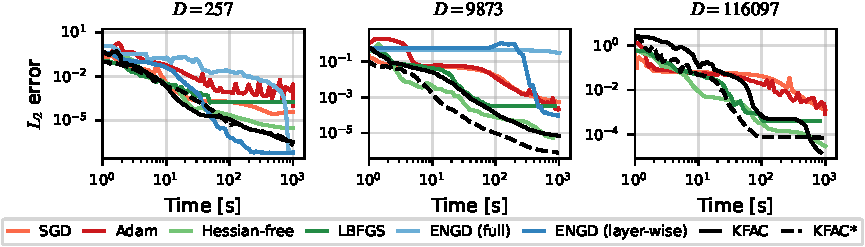
\includegraphics{../kfac_pinns_exp/exp17_groupplot_poisson2d/l2_error_over_time.pdf}
    \caption{We report the performance of different optimizers on the Poisson equation~\eqref{eq:2D-Poisson} measured in relative $L^2$ error against wall clock time for architectures with different parameter dimensions $D$; ...}
    \label{fig:2D-Poisson}
\end{figure}


\subsection{A higher-dimensional evolutionary problem}

To demonstrate that our method can also be applied to other problems as the Poisson equation we consider the four-dimensional heat equation 
\begin{align}
    asdf.
\end{align}
Like before, we evaluate the performance of the different optimizers for networks with $4$ hidden layers, $\tanh$ activation function, and layers of different sizes. 
We report the relative $L^2$ error with respect to the optimization time in \Cref{fig:4D-heat}.  
 
\begin{figure}
    \centering
    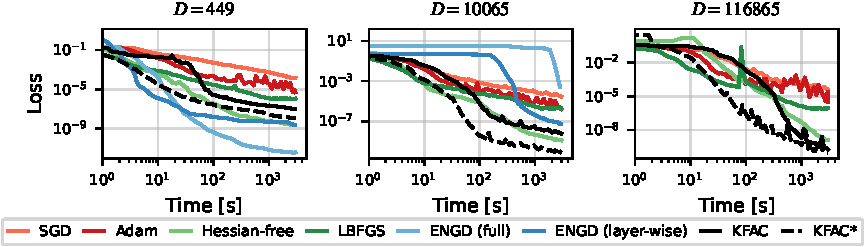
\includegraphics{../kfac_pinns_exp/exp30_heat4d_groupplot/loss_over_time.pdf}
    \caption{We report the performance of different optimizers on the Poisson equation~\eqref{eq:2D-Poisson} measured in relative $L^2$ error against wall clock time for architectures with different parameter dimensions $D$; ...}
    \label{fig:4D-heat}
\end{figure}

%\subsection{A 10D Poisson equation}

%\begin{align}
%    \begin{split}
%        asdf
%    \end{split}
%\end{align}

%\todo[inline]{I think we should only present the time plots to safe space, move everything else to the appendix}

\begin{comment}
    \subsection{A 100D Poisson equation}

\begin{itemize}
\item 100D from deep Ritz paper~\citep{yu2018deep}, i.e.,
  \begin{align*}
    -\Delta u(x) & = -200 \quad \text{for } x\in [0,1]^{100} \\
    u(x) & = \lVert x \rVert_2^2 \quad \text{for } x\in \partial[0,1]^{100}
  \end{align*}
  where the solution is given by $u^\star(x) = \lVert x \rVert_2^2$
\item around $10^5$ to $10^6$ parameters
\item no ENGD, ENGD matrix-free?, only KFACs, L-BFGS, HF, and first-order methods
\end{itemize}


    \subsection{Heat equation}

\begin{itemize}
\item again 100D
\item sum of cosinuts with exponential trash in time? I.e.,
  time-space domain $[0,1]\times[0,1]^{100}$ %and
  % \begin{align*}
  %   \partial_t u(t,x)-\Delta_x u(t,x) & = 0 \quad \text{for } x\in [0,1]^{100} \\
      %       u(0,x) & = \sum_{i=1}^{100} \sin(\pi x_i) \quad \text{for }
  %   x\in [0,1]^{100}
  %   \\
  %   u(t,x) & = 0 \quad \text{for } t\in[0,1], x\in\partial[0,1]^{100}
  % \end{align*}
  % \item an alternative would be
  \todo{rhs not equal zero I think, double check before implementing}
  \begin{align*}
    \partial_t u(t,x)-\Delta_x u(t,x) & = 0 \quad \text{for } x\in [0,1]^{100} \\
    u(0,x) & = \sum_{i=1}^{100} \sin(\pi x_i) \quad \text{for }
             x\in [0,1]^{100}
    \\
    u(t,x) & = e^{-\pi^2 t}\sum_{i=1}^{100} \sin(\pi x_i) \quad \text{for } t\in[0,1], x\in\partial[0,1]^{100}
  \end{align*}
  for which the solution should be given by
  \begin{align*}
    u^\star(t,x) = e^{-\pi^2 t} \sum_{i=1}^{100} \sin(\pi x_i)?
  \end{align*}
  % we can also scale in time because $e^{-4\pi^2}\approx e^{-40}$
\item around $10^5-10^6$ parameters
\end{itemize}
\end{comment}

\subsection{Discussion}

Hessian free vs KFAC (KFAC plays nicer with stochasticity?!)

\begin{itemize}
    \item KFAC is competitive with exact second-order methods on smaller scale networks
    \item ... 
\end{itemize}

%\subsection{Limitations and Future Work}

\paragraph{Limitations}
\paragraph{Studying further KFAC heuristics} The original KFAC optimizer introduces many additional techniques to improve performance and stability, e.g.\,adaptive damping and heuristics for splitting up the damping onto the different Kronecker factors.
Our algorithms borrow components, but we did not explore all bells and whistles.
We believe they can help to either reduce the number of hyper-parameters that need to be tuned, or improve performance.
We use an independent Kronecker product for each of the losses and dit not look into further condensing this representation into a single Kronecker product.
Doing so would allow to further reduce memory cost for storing the pre-conditioner, as well as computational cost to invert it.
We did not play around with updating the KFAC matrices or inverting the pre-conditioner less frequently.
We did not try lower precision than float64 because this is the standard setup for PINNs (??).

\paragraph{Performance improvements} The generalized eigenvalue that we currently need to solve to invert the Kronecker sum is currently computed through SciPy as there is no PyTorch API for doing so. This has the downside that we need to sync the Kronecker factors with CPU each time we want to invert the curvature approximation. Our results could be further improved by using a fully GPU-compatible implementation.
As pointed out in \citep{martens2015optimizing}, the requested Gramian projections can be computed at the cost of two forward passes; however, we are currently using a non-specialized implementation which does not take into account the Gramian's matrix square root factorization.
One could also merge the backward pass for each Gramian with that of its loss into a single backward traversal rather than two sequential ones, e.g.\,as done by~\cite{dangel2020backpack}.
However, then one needs to manually implement the additional backpropagation (through both the normal forward pass, but also through the forward Laplacian pass).

\paragraph{Future work}
Inverse-free KFAC update~\citep{lin2023simplifying} and structured Kronecker factors~\citep{lin2023structured}.

\begin{comment}
  We want to show the following things:
  \begin{itemize}
  \item We can safely discard the Gramian's off-diagonal blocks without harming
    training performance. This reduces the Gramian's size, but still imposes
    strong constraints on scalability.

  \item Our proposed Kronecker approximation works roughly as well as the
    full/block diagonal Gramian, while being much cheaper to compute, store, and
    invert.

  \item Thanks to the Kronecker approximation of the Gramian, we can scale to larger neural networks where the other methods either do not work (storing the Gramian is prohibitively expensive) or become quite slow (matrix-free linear system solve via Gramian-vector products).
  \end{itemize}

  Todos:
  \begin{itemize}
  \item concrete example ground truth: 2d Poisson on unit square with sine target
  \end{itemize}

  Ideas:
  \begin{itemize}
  \item try out different approximations
    \begin{itemize}
    \item Ground truth
    \item Block diagonal exact
    \item Diagonal
    \item Block diagonal with different approximations
    \end{itemize}
  \end{itemize}
\end{comment}

%%% Local Variables:
%%% mode: latex
%%% TeX-master: "../main"
%%% End:


\section{Discussion and Conclusion}\label{sec:conclusion}

%We provide KFAC approximations for preconditioners involving general PDE terms
%This builds on an interpretation of the input-derivatives of a network via Taylor-mode automatic differentiation as a weight-sharing network.
%We provide an efficient implementation of the proposed KFAC method and demonstrate that i t...?
We propose KFAC-methods for PINN losses that greatly reduces the computational cost and allows scaling to much larger networks.
Our approach goes beyond the popular KFAC for traditional deep learning problems as it captures contributions from a PDE's differential operator that are crucial for optimization.
To establish KFAC for such losses, we use Taylor-mode automatic differentiation to describe the differential operator's computation graph as a forward network with shared weights which allows us to apply a variant of KFAC for networks with weight-sharing.
Empirically, we find that our KFAC-based optimizers are competitive with expensive second-order methods on small problems, scale more favorably to higher-dimensional neural networks and PDEs, and consistently outperform first-order methods.

\paragraph{Limitations and future directions}
Currently, our KFAC approximations can only handle feedforward architectures, where it is natural to extend them to more general architectures in the future.
Further, optimizing our implementation using inverse-free KFAC update~\citep{lin2023simplifying}, structured Kronecker factors~\citep{lin2023structured}, and more sophisticated heuristics would likely improve the proposed method.
It remains to test the performance of our proposed approximation when applied to the optimization of larger networks and more PDEs including nonlinear problems.
\begin{itemize}
    \item improve heuristics
    \item
\end{itemize}


\paragraph{Studying further KFAC heuristics} The original KFAC optimizer introduces many additional techniques to improve performance and stability, e.g.\,adaptive damping and heuristics for splitting up the damping onto the different Kronecker factors.
Our algorithms borrow components, but we did not explore all bells and whistles.
We believe they can help to either reduce the number of hyper-parameters that need to be tuned, or improve performance.
We use an independent Kronecker product for each of the losses and dit not look into further condensing this representation into a single Kronecker product.
Doing so would allow to further reduce memory cost for storing the preconditioner, as well as computational cost to invert it.
We did not play around with updating the KFAC matrices or inverting the preconditioner less frequently.
We did not try lower precision than float64 because this is the standard setup for PINNs (??).

\paragraph{Performance improvements} The generalized eigenvalue that we currently need to solve to invert the Kronecker sum is currently computed through SciPy as there is no PyTorch API for doing so. This has the downside that we need to sync the Kronecker factors with CPU each time we want to invert the curvature approximation. Our results could be further improved by using a fully GPU-compatible implementation.
As pointed out in \citep{martens2015optimizing}, the requested Gramian projections can be computed at the cost of two forward passes; however, we are currently using a non-specialized implementation which does not take into account the Gramian's matrix square root factorization.
One could also merge the backward pass for each Gramian with that of its loss into a single backward traversal rather than two sequential ones, e.g.\,as done by~\cite{dangel2020backpack}.
However, then one needs to manually implement the additional backpropagation (through both the normal forward pass, but also through the forward Laplacian pass).




%\begin{itemize}
    %\item Only works for sequential networks
    %\item Hessian backpropagation requires memory quadratic in the intermediate features size and therefore becomes impractical for large intermediates like in CNNs.
    %\item Our implementation is likely manual and relatively hard to automate with the current graph inspection tools offered by ML frameworks.
%    \item bigger networks
%    \item harder, nonlinear PDEs
%\end{itemize}



%%% Local Variables:
%%% mode: latex
%%% TeX-master: "../main"
%%% End:

\begin{ack} % automatically suppressed in anonymized submission
  The authors thank Runa Eschenhagen for insightful discussions on KFAC for linear weight sharing layers.
  FD would like to thank Luca Thiede for his adamant questions about Taylor mode and forward Laplacians.
  Resources used in preparing this research were provided, in part, by the Province of Ontario, the Government of Canada through CIFAR, and companies sponsoring the Vector Institute.
  JM acknowledges funding by the Deutsche Forschungsgemeinschaft (DFG, German Research Foundation) under the project number 442047500 through the Collaborative Research Center \emph{Sparsity and Singular Structures} (SFB 1481).
  MZ acknowledges support from an ETH Postdoctoral Fellowship for the project ``Reliable, Efficient, and Scalable Methods for Scientific Machine Learning''.
\end{ack}
%%% Local Variables:
%%% mode: latex
%%% TeX-master: "../main"
%%% End:


\bibliography{references}
\bibliographystyle{icml2024.bst}

\clearpage
\appendix

\clearpage

% Use different numbering in appendix to make it clear that a
% section/table/algorithm is not in the main text
\renewcommand\thefigure{\thesection\arabic{figure}}
\renewcommand\thetable{\thesection\arabic{table}}
\renewcommand{\theequation}{\thesection\arabic{equation}}

% modified title header from main page, code extracted from NeurIPS template
\makeatletter
\vbox{%
  \hsize\textwidth
  \linewidth\hsize
  \vskip 0.1in
  \@toptitlebar
  \centering
  {\LARGE\bf \@title (Supplementary Material)\par}
  \@bottomtitlebar
  \vskip 0.3in \@minus 0.1in
}
\makeatother

% APPENDIX TOC
\startcontents[sections]
\printcontents[sections]{l}{1}{\setcounter{tocdepth}{2}}
\vspace{2em}

\section{The Computations for the Different KFACs}
\begin{equation*}
    \mG_\Omega(\mW^{(l)})
    =
    \frac1N\sum_{n=1}^N
    \left[\sum_{s=1}^S \left( \mZ^{(l-1)}_{n,s}\otimes \vg_{n,s}^{(l)} \right)
    \cdot
    \sum_{s=1}^S \left( \mZ
    ^{(l-1)}_{n,s}\otimes \vg_{n,s}^{(l)} \right)^\top\right]
\end{equation*}

%
%\paragraph{Kronecker approximation of the PDE Gramian}

\paragraph{The reduce approximation}
Approximating the sum of Kronecker products (running over $s$) by the Kronecker product of the sum, simplifying and again approximating for the outer sum (running over $n$) we obtain
\begin{align*}
    \hat{\mG}_\Omega^{\textup{red}}(\mW^{(l)})
    \coloneqq
    \frac{1}{N^2 S^2} \left[\sum_{n=1}^N \left( \sum_{s=1}^S \mZ^{(l-1)}_{n,s} \right) \left(\sum_{s=1}^S {\mZ^{(l-1)}_{n,s}}\right)^\top\right]
    \otimes
    \left[\sum_{n=1}^N\left(\sum_{s=1}^S \vg^{(l)}_{n,s} \right) \left( \sum_{s=1}^S {\vg^{(l)}_{n,s}} \right)^\top \right]
\end{align*}
This approximation agrees with the \emph{reduce} setting described by~\citet{eschenhagen2023kroneckerfactored}.

\paragraph{Individual steps} Can be moved to the appendix or deleted:

\begin{align*}
    &\; \sum_{n=1}^N
    \left[\sum_{s=1}^S \left( \mZ^{(l-1)}_{n,s}\otimes \vg_{n,s}^{(l)} \right)
    \cdot
    \sum_{s=1}^S \left( \mZ
    ^{(l-1)}_{n,s}\otimes \vg_{n,s}^{(l)} \right)^\top\right]
    \\ \approx & \;
    \sum_{n=1}^N
    \frac{1}{S^2}\left[\left(\left( \sum_{s=1}^S\mZ^{(l-1)}_{n,s}\right)\otimes \left(\sum_{s=1}^S\vg_{n,s}^{(l)}\right)\right)
    \cdot
    \left(\left( \sum_{s=1}^S\mZ^{(l-1)}_{n,s}\right)^\top\otimes \left(\sum_{s=1}^S\vg_{n,s}^{(l)}\right)^\top\right)\right]
    \\ = & \;
    \frac{1}{S^2}\sum_{n=1}^N
    \left[\left(\left( \sum_{s=1}^S\mZ^{(l-1)}_{n,s}\right)\left( \sum_{s=1}^S\mZ^{(l-1)}_{n,s}\right)^\top \right)\otimes \left(\left(\sum_{s=1}^S\vg_{n,s}^{(l)}\right)\left(\sum_{s=1}^S\vg_{n,s}^{(l)}\right)^\top\right)
     \right]
    \\ \approx & \;
    \frac{1}{N S^2}\left[\sum_{n=1}^N \left( \sum_{s=1}^S \mZ^{(l-1)}_{n,s} \right) \left(\sum_{s=1}^S {\mZ^{(l-1)}_{n,s}}\right)^\top\right]
    \otimes
    \left[\sum_{n=1}^N\left(\sum_{s=1}^S \vg^{(l)}_{n,s} \right) \left( \sum_{s=1}^S {\vg^{(l)}_{n,s}} \right)^\top \right]
\end{align*}


\paragraph{The expand approximation}
Alternatively, approximating the inner matrix product of sums in equation~\eqref{eq:laplace_gramian_block_exact} by the sum of matrix products, simplifying, and approximating the sum of Kroneckers by the Kronecker of the sum we obtain
\begin{align*}
    \hat{\mG}_\Omega^{\textup{exp}}(\mW^{(l)})
    \coloneqq \frac{1}{N^2 S}
    \left[\sum_{n=1}^N \sum_{s=1}^S \mZ^{(l-1)}_{n,s}{\mZ^{(l-1)}_{n,s}}^\top \right]
    \otimes
    \left[\sum_{n=1}^N\sum_{s=1}^S \vg^{(l)}_{n,s}{\vg^{(l)}_{n,s}}^\top   \right].
\end{align*}
which coincides with the \emph{expand} setting of \cite{eschenhagen2023kroneckerfactored}. 

\paragraph{Individual steps} 
An alternative to the approximation above, one can use the approximation $\sum_{n}A_n\sum_n B_n \approx N^{-1}\sum_{n}A_nB_n$ to get 
\begin{align*}
    & \sum_{n=1}^N
    \left[\sum_{s=1}^S \left( \mZ^{(l-1)}_{n,s}\otimes \vg_{n,s}^{(l)} \right)
    \cdot
    \sum_{s=1}^S \left( \mZ
    ^{(l-1)}_{n,s}\otimes \vg_{n,s}^{(l)} \right)^\top\right]
    \\ \approx & \;
    \frac{1}{S?}\sum_{n=1}^N
    \left[\sum_{s=1}^S \left( \mZ^{(l-1)}_{n,s}\otimes \vg_{n,s}^{(l)} \right)
    \cdot
    \left( \mZ
    ^{(l-1)}_{n,s}\otimes \vg_{n,s}^{(l)} \right)^\top\right]
    \\ = & \;
    \frac{1}{S}\sum_{n=1}^N
    \left[\sum_{s=1}^S \left( \mZ^{(l-1)}_{n,s}{\mZ
    ^{(l-1)}_{n,s}}^\top\otimes \vg_{n,s}^{(l)}{\vg_{n,s}^{(l)}}^\top \right)
    \right]
    \\ \approx & \;
    \frac{1}{NS}\left[\sum_{n=1}^N \sum_{s=1}^S \mZ^{(l-1)}_{n,s}{\mZ^{(l-1)}_{n,s}}^\top \right]
    \otimes
    \left[\sum_{n=1}^N\sum_{s=1}^S \vg^{(l)}_{n,s}{\vg^{(l)}_{n,s}}^\top \right].
\end{align*}


\section{Pseudo-Code: KFAC for the Poisson Equation}
\begin{algorithm}[!h]
  \centering
  \begin{small}
    \begin{algorithmic}
      \Require \\
      MLP $u_{\vtheta}$ with parameters $\vtheta_0 = (\vtheta_0^{(1)}, \dots, \vtheta_0^{(L)}) = (\flatten \mW_0^{(1)}, \dots, \flatten \mW_0^{(L)}) $, \\
      interior data $\{(\vx_n, y_n) \}_{n=1}^{N_{\Omega}}$, \\
      boundary data $\{(\vx^{\text{b}}_n, y^{\text{b}}_n) \}_{n=1}^{N_{\partial\Omega}}$ \\
      exponential moving average $\beta$, momentum $\mu$, Damping $\lambda$, number of steps $T$

      \\
      \State \textbf{0) Initialization}
      \For {$l=1, \dots, L$}
        \State $\mA_{\Omega}^{(l)}, \mB_{\Omega}^{(l)}, \mA_{\partial\Omega}^{(l)}, \mB_{\partial\Omega}^{(l)} \gets \vzero \text{ or } \mI$ \Comment Initialize Kronecker factors
      \EndFor
      \\
      \For {$t = 0, \dots, T-1$}
        \\
        \State \textbf{1) Compute the interior loss and update its approximate curvature}
        \State $(\mZ_n^{(0)}\dots, \mZ_n^{(L)}, \Delta u_n) \gets \Delta u_{\vtheta_t}(\vx_n)\quad n=1, \dots, N_{\Omega}$  \Comment Forward Laplacian wit intermediates

        \State Compute layer output gradients $\vg^{(l)}_{n,s} \coloneqq \nicefrac{\partial \Delta u_n}{\partial\mZ_{n,s}^{(l)}}$ with autodiff in one backward pass
        \State $(\vg_{n,s}^{(1)}, \dots, \vg_{n,s}^{(L)}) \gets \texttt{grad}(\Delta u_n, (\mZ_{n,s}^{(1)}, \dots, \mZ_{n,s}^{(L)}))\quad n=1, \dots, N_{\Omega}$, \quad $s = 1, \dots, S \coloneqq d+2$

        \ForAll{$l=1, \dots, L$} \Comment Update Kronecker factors of the interior loss
          \State $\hat{\mA}_{\Omega}^{(l)} \gets \beta \hat{\mA}_{\Omega}^{(l)} + (1-\beta) \frac1{N_{\Omega} S} \sum_{n=1}^{N_{\Omega}} \mZ_{n,s}^{(l-1)} \mZ_{n,s}^{(l-1)\top}$

          \State $\hat{\mB}_{\Omega}^{(l)} \gets \beta \hat{\mB}_{\Omega}^{(l)} + (1-\beta) \frac1{N_{\Omega}} \sum_{n=1}^{N_{\Omega}} \vg^{(l)}_{n,s} \vg^{(l)\top}_{n,s}$
        \EndFor

        \State $L_{\Omega}(\vtheta_t) \gets \frac{1}{2 N_{\Omega}}\sum_{n=1}^{N_{\Omega}} (\Delta u_n - y_n)^2$ \Comment Compute interior loss

        \\
        \State \textbf{2) Compute the boundary loss and update its approximate curvature}
        \State $(\vz_n^{(0)}\dots, \vz_n^{(L)}, u_n) \gets u_{\vtheta_t}(\vx_n^{\text{b}})\quad n=1, \dots, N_{\partial\Omega}$ \Comment Forward pass with intermediates
        \State Compute layer output gradients $\vg_n^{(l)} \coloneqq \nicefrac{\partial u_n}{\vz^{(l)}_n}$ with autodiff in one backward pass
        \State $(\vg_n^{(1)}\dots, \partial\vg_n^{(L)}) \gets \texttt{grad}(u_n, (\vz_n^{(0)}\dots, \vz_n^{(L)}))\quad n=1, \dots, N_{\partial\Omega}$

        \ForAll{$l=1, \dots, L$} \Comment Update Kronecker factors of the boundary loss
          \State $\hat{\mA}_{\partial\Omega}^{(l)} \gets \beta \hat{\mA}_{\partial\Omega}^{(l)} + (1-\beta) \frac1{N_{\partial\Omega}} \sum_{n=1}^{N_{\partial\Omega}} \vz_n^{(l-1)} \vz_n^{(l-1)\top}$

          \State $\hat{\mB}_{\partial\Omega}^{(l)} \gets \beta \hat{\mB}_{\partial\Omega}^{(l)} + (1-\beta) \frac1{N_{\partial\Omega}} \sum_{n=1}^{N_{\partial\Omega}} \vg_n^{(l)} \vg_n^{(l)\top}$
        \EndFor

        \State $L_{\partial\Omega}(\vtheta_t) \gets \frac{1}{2 N_{\partial\Omega}}\sum_{n=1}^{N_{\partial\Omega}} (u_n - y^{\text{b}}_n)^2$ \Comment Compute boundary loss

        \\
        \State \textbf{3) Update the preconditioner (use inverse of Kronecker sum trick)}
        \ForAll{$l=1, \dots, L$}
          \State $ \mC^{(l)} \gets \left[(\hat{\mA}_{\Omega}^{(l)} + \lambda \mI) \otimes (\hat{\mB}_{\Omega}^{(l)} + \lambda \mI) + (\hat{\mA}_{\partial\Omega}^{(l)} + \lambda \mI) \otimes (\hat{\mB}_{\partial\Omega}^{(l)} + \lambda \mI)  \right]^{-1}$
        \EndFor

        \\
        \State \textbf{4) Compute the gradient using autodiff, precondition the gradient}
        \State $(\vg^{(1)}, \dots, \vg^{(L)}) \gets \texttt{grad}( L_{\Omega}(\vtheta_t) + L_{\partial\Omega}(\vtheta_t), (\vtheta_t^{(1)}, \dots, \vtheta^{(L)}_t ))$ \Comment Gradient with autodiff

        \ForAll{$l=1, \dots, L$}
          \Comment Precondition gradient
          \State $\vDelta_t \gets - \mC^{(l)} \vg^{(l)}$ \Comment Proposed update direction
          \State $\hat{\vdelta}_t^{(l)} \gets \mu \vdelta_{t-1}^{(l)} + \vDelta_t^{(l)} \text{ if $t>0$ else } \vDelta_t^{(l)}$ \Comment Add momentum from previous update
        \EndFor

        \\
        \State \textbf{5) Given the direction $\hat{\vdelta}_t^{(1)}, \dots, \hat{\vdelta}_t^{(L)}$, choose learning rate $\alpha$ by line search \& update}
        \For {$l=1, \dots, L$} \Comment Parameter update
          \State $\vdelta_t^{(l)} \gets \alpha \hat{\vdelta}_t^{(l)}$
          \State $\vtheta^{(l)}_{t+1} \gets \vtheta^{(l)}_t + \alpha \vdelta_t^{(l)}$
        \EndFor
      \EndFor

      \\
      \State \Return Trained parameters $\vtheta_T$
    \end{algorithmic}
  \end{small}
    \caption{KFAC for the Poisson equation.}
\end{algorithm}
%%% Local Variables:
%%% mode: latex
%%% TeX-master: "../main"
%%% End:


%\section{Example: Laplacian for a Shallow Network}
%

\section{Example: Laplacian for a Shallow Network}

Here, we compute the Laplacian for a less general, yet simpler, example: A shallow neural network.

\begin{comment}
  For the one-dimensional shallow case we have
  \[ u_\theta(x) = \sum_{i=1}^m a_i\sigma(b_i x + c_i) + d. \]
  Then
  \[ u_\theta'(x) = \sum_{i=1}^m a_ib_i\sigma'(b_i x + c_i) \]
  and
  \[ u_\theta''(x) = \sum_{i=1}^m a_ib_i^2\sigma''(b_i x + c_i). \]
  The parameter derivative of the Laplacian (i.e., second-order derivative)
  \begin{align*}
    \partial_{a_i}u_\theta''(x) & = b_i^2\sigma''(b_i x + c_i) \\
    \partial_{b_i}u_\theta''(x) & = 2a_ib_i\sigma''(b_i x + c_i) + a_i b_i^2x\sigma^{(3)}(b_i x + c_i) \\
    \partial_{c_i}u_\theta''(x) & = a_i b_i^2\sigma^{(3)}(b_i x + c_i) \\
    \partial_{d}u_\theta''(x) & = 0.
  \end{align*}
  The parameter derivative of the Laplacian (i.e., second-order derivative)
  \begin{align*}
    \partial_{a_i}u_\theta''(x) & = b_i^2\sigma''(b_i x + c_i) \\
    \partial_{b_i}u_\theta''(x) & = 2a_ib_i\sigma''(b_i x + c_i) + a_i b_i^2x\sigma^{(3)}(b_i x + c_i) \\
    \partial_{c_i}u_\theta''(x) & = a_i b_i^2\sigma^{(3)}(b_i x + c_i) \\
    \partial_{d}u_\theta''(x) & = 0.
  \end{align*}
\end{comment}

First, we do the Hessian calculation as explicitly as possible. For this, we consider the easy case of a shallow network with one-dimensional output
\[ u_\theta(x) = \sum_{i=1}^m a_i\sigma(b_i^\top x + c_i) + d. \]
Then
\[ \nabla_x u_\theta(x) = \sum_{i=1}^m a_ib_i\sigma'(b_i x + c_i) \]
or
\[ \partial_{x_j} u_\theta(x) = \sum_{i=1}^m a_i(b_i)_j\sigma'(b_i x + c_i). \]
Consequently, we compute
\[ \partial_{x_k}\partial_{x_j} u_\theta(x) = \sum_{i=1}^m a_i(b_i)_j(b_i)_k\sigma'(b_i x + c_i) \]
which yields the Hessian
\[ \nabla^2_x u_\theta(x) = \sum_{i=1}^m a_i\sigma''(b_i x + c_i) \cdot b_ib_i^\top = \sum_{i=1}^m a_i\sigma''(b_i x + c_i) \cdot  b_i\otimes b_i \]
and the Laplacian is given by
\[ \Delta_x u_\theta(x) = \sum_{i=1}^m a_i\sigma''(b_i x + c_i) \operatorname{tr}(b_ib_i^\top) = \sum_{i=1}^m a_i\sigma''(b_i x + c_i)  \operatorname{tr}(b_i\otimes b_i). \]
The parameter derivatives of the Hessian are given
\begin{align*}
  \partial_{a_i}\nabla_x^2 u_\theta(x) & = \sigma''(b_i x + c_i) b_ib_i^\top \\
  \nabla_{b_i}\nabla_x^2 u_\theta(x) & = a_i\sigma''(b_i x + c_i) (b_i\otimes I+I\otimes b_i) + a_i \sigma^{(3)}(b_i x + c_i) \cdot  (I\otimes x^\top)(b_i\otimes b_i) \quad ?? \\
  % + a_i x\sigma^{(3)}(b_i x + c_i) \cdot b_ib_i^\top \\
     \partial_{c_i}\nabla_x^2 u_\theta(x) & = a_i b_i^2\sigma^{(3)}(b_i x + c_i) \\
     \partial_{d}\nabla_x^2 u_\theta(x) & = 0.
\end{align*}
The parameter derivatives of the Laplacian are given
\begin{align*}
     \partial_{a_i}\Delta_x u_\theta(x) & = \sigma''(b_i x + c_i) \operatorname{tr}(b_ib_i^\top) \\
     \nabla_{b_i}\Delta_x u_\theta(x) & = 2a_i\sigma''(b_i x + c_i) + a_i \sigma^{(3)}(b_i x + c_i) \operatorname{tr}(b_ib_i^\top) \cdot x \\
     \partial_{c_i}\Delta_x u_\theta(x) & = a_i \sigma^{(3)}(b_i x + c_i)\operatorname{tr}(b_ib_i^\top) \\
     \partial_{d}\Delta_x u_\theta(x) & = 0.
\end{align*}


\paragraph{Writing as linear algebra}

Consider a shallow network
\[ u_\theta(x) = W_2\sigma(W_1 x), \]
where $x\in\mathbb R^d$, $W_1\in\mathbb R^{m\times d}, W_2\in\mathbb R^{1\times m}$.

\paragraph{Task: }
Understand the structure, in particular the computational graph of $f_\theta = \Delta u_\theta$.

\paragraph{One dimensional case: }
Assume first that $d=1$.
Then
\[ D_x u_\theta(x) = W_2 \operatorname{diag}(\sigma'(W_1 x)) W_1 \]
and
\[ D^2_x u_\theta(x) = W_2%(W_1^\top\otimes W_2)
  \operatorname{diag}(\operatorname{diag}(\sigma''(W_1 x)) W_1)W_1. % = W_2 \operatorname{diag}\sigma''(W_1 x) W_1^2 = W_2\odot W_1^2 \sigma''(W_1x),
\]
In another form
\[D^2 u_\theta(x) = W_2 \operatorname{diag}(\operatorname{diag}\sigma''(W_1 x) W_1) W_1 = W_2 \operatorname{diag}\sigma''(W_1 x) W_1^2 = W_2\odot W_1^2 \sigma''(W_1x),
\]
where $(W_2\odot W_1^2)_k = (W_2)_k \cdot (W_1)_k^2$.
% where $(W_2\odot W_1^2)_k = (W_2)_k \cdot (W_1)_k^2$.
% The Laplacian is then given as
% \[ f_\theta(x) = \Delta u_\theta(x) = \operatorname{tr}(D_x^2u_\theta(x)) =\operatorname{tr}(W_2 \operatorname{diag}(\operatorname{diag}(\sigma''(W_1 x)) W_1) W_1).  \]
% Differentiation with respect to $W_2$ yields
% \[ \frac{\partial f_\theta(x)}{\partial W_2} = \frac{\partial \Delta u_\theta(x)}{ \partial W_2} =  \]

One can also rewrite the diagonalization operator via a Hadamard product as $\operatorname{diag}(x) = (x\mathds{1}^\top)\odot I$, where $\mathds{1}$ denotes the all one vector, $I$ the identity and $\odot$ the Hadamard (i.e., entrywise) product of two matrices.
Not sure whether this helps though...

\paragraph{Multi-dimensional case}

%%% Local Variables:
%%% mode: latex
%%% TeX-master: "../main"
%%% End:


\section{Inverting the Sum of Two Kronecker Matrices}\label{sec:inverse_kronecker_sum}
PINNs use two losses: a boundary and an interior loss.
When designing a Kronecker-factored curvature approximation, we have two choices:
\begin{enumerate}
\item We can approximate each loss individually with a Kronecker product, i.e.
  \begin{align*}
    \mK \coloneqq \mA_1 \otimes \mA_2 + \mB_1 \otimes \mB_2
  \end{align*}
  where $\mA_{1,2}, \mB_{1,2}$ are invertible and positive definite.

\item We can further approximate the above through a single Kronecker product, e.g.\,by summing,
  \begin{align*}
    \mK' \coloneqq (\mA_1 + \mB_1) \otimes (\mA_2 + \mB_2) \approx \mK\,.
  \end{align*}
\end{enumerate}
Eventually, we want to use their inverses.
For $\mK'$, this is straightforward to do.
For $\mK$, we need to invert the sum of two Kronecker products, which is more challenging.
We can proceed as follows to invert $\mK$:
\begin{enumerate}
\item Simultaneously diagonalize $(\mA_i, \mB_i)$ by solving the generalized eigenvalue problem
  \begin{align*}
    \mA_i \mV_i = \mB \mV_i \mLambda_i
  \end{align*}
  where $\mV_i$'s columns are the (generalized) eigenvectors and $\mLambda_i$ is a diagonal matrix containing the (generalized) eigenvalues.

\item Consider the expression
  \begin{align*}
    &\left(
      \mA_1 \otimes \mA_2
      +
      \mB_1 \otimes \mB_2
      \right)
      \left(
      \mV_1 \otimes \mV_2
      \right)
    \\
    &=
      \mB_1 \mV_1 \mLambda_1 \otimes \mB_2 \mV_2 \mLambda_2
      +
      \left( \mB_1 \otimes \mB_2 \right)
      \left( \mV_1 \otimes \mV_2 \right)
    \\
    &=
      \left( \mB_1 \otimes \mB_2 \right)
      \left( \mV_1 \otimes \mV_2 \right)
      \left(
      \mLambda_1 \otimes \mLambda_2 + \mI \otimes \mI
      \right)\,.
  \end{align*}
  Rearrange into
  \begin{align*}
    \left(
    \mA_1 \otimes \mA_2
    +
    \mB_1 \otimes \mB_2
    \right)
    =
    \left( \mB_1 \otimes \mB_2 \right)
    \left( \mV_1 \otimes \mV_2 \right)
    \left(
    \mLambda_1 \otimes \mLambda_2 + \mI \otimes \mI
    \right)
    \left( \mV_1^{-1} \otimes \mV_2^{-1} \right)
    \,.
  \end{align*}

  \item Take the inverse to obtain
    \begin{align*}
      \mK^{-1}
      =
      \left( \mV_1 \otimes \mV_2 \right)
      \left(
      \mLambda_1 \otimes \mLambda_2 + \mI \otimes \mI
      \right)^{-1}
      \left( \mV_1^{-1}\mB_1^{-1} \otimes \mV_2^{-1}\mB_2^{-1} \right)
      \,.
    \end{align*}
    Notice that $\mLambda_1 \otimes \mLambda_2 + \mI \otimes \mI$ is diagonal, and therefore easy to invert.
\end{enumerate}

%%% Local Variables:
%%% mode: latex
%%% TeX-master: "../main"
%%% End:


%\section{Heat Equation}\label{sec:heat_equation}
%Consider the $D$-dimensional\todo{Low priority: lower case $d$ or upper case $D$? The number of trainable weights is already $D$.} homogeneous heat equation
\begin{align*}
  \partial_{t} u(t, \vx)
  -
  \kappa \Delta_{\vx} u(t, \vx)
  =
  0
\end{align*}
where $\vx \in \Omega \subseteq \sR^D$, $t \in \mathrm{T} \subseteq \sR$ is a time interval, and $\kappa >0$ denotes the heat conductivity. In this case, our neural network processes a $D+1$-dimensional vector $\tilde{\vx} =
\begin{pmatrix} t \\ \vx \end{pmatrix}$ and we can re-write the heat equation as
\begin{align*}
  \partial_{[\tilde{\vx}]_1} u(\tilde{\vx})
  -
  \kappa \sum_{d=2}^{D+1} \Delta_{[\tilde{\vx}]_d} u(\tilde{\vx})
  =
  0\,.
\end{align*}
In the following, we consider the unit time interval $\mathrm{T} = [0;1]$, the unit square $\Omega = [0;1]^D$ and set $\kappa = \nicefrac{1}{4}$. There are two types of constraints we need to enforce on the heat equation in order to obtain unique solutions: initial conditions and boundary conditions. As our framework for the KFAC approximation assumes only two terms in the loss function, we combine the contributions from the boundary and initial values into one term. To make this more precise consider the following example solution of the heat equation, which will be used later on as well.
As initial conditions, we use $u_0(x) = u(0, \vx) = \prod_{d=1}^D \sin(\pi [\vx_d])$ for $\vx \in \Omega$.
For boundary conditions, we use $g(t, \vx) = 0$ for $t, \vx \in \mathrm{T} \times \partial\Omega$.
The manufactured solution thus is
\begin{align*}
  u^{\star}(t, \vx)
  =
  \exp \left(-\frac{\pi^2 D t}{4} \right)
  \prod_{d=1}^D \sin(\pi [\vx_d])\,.
\end{align*}
The PINN loss for this problem consists of three terms
\begin{align*}
  \gL(\vtheta)
  &=
    \frac{1}{N_{\Omega}}
    \sum_{n=1}^{N_{\Omega}}
    \left\lVert
    \partial_t u_{\vtheta}(\tilde{\vx}_n^{\Omega})
    -
    \frac{1}{4} \Delta_{\vx} u_{\vtheta}(\tilde{\vx}_n^{\Omega})
    \right\rVert^2_2
  \\
  &+
    \frac{1}{N_{\partial\Omega}}
    \sum_{n=1}^{N_{\partial\Omega}}
    \left\lVert
    u_{\vtheta}(\tilde{\vx}_n^{\partial\Omega})
    -
    g(\tilde{\vx}_n^{\partial\Omega})
    \right\rVert^2_2
  \\
  &+
    \frac{1}{N_0}
    \sum_{n=1}^{N_0}
    \left\lVert
    u_{\vtheta}(0, \vx_n^0)
    -
    u_0( \vx_n^0)
    \right\rVert^2_2
\end{align*}
with $\tilde{\vx}_n^{\Omega} \sim \mathrm{T} \times \Omega$, and $\tilde{\vx}_n^{\partial\Omega} \sim \mathrm{T} \times \partial\Omega$, and $\vx_n^0 \sim \{0\} \times \Omega$.
To fit this loss into our framework which assumes two loss terms, each of whose curvature is approximated with a Kronecker factor, we combine the initial value and boundary value conditions into a single term.
Assuming $N_{\partial \Omega} = N_0 = \nicefrac{N_{\text{cond}}}{2}$ without loss of generality, we write
\begin{align*}
  \gL(\vtheta)
  &=
    \underbrace{
    \frac{1}{N_{\Omega}}
    \sum_{n=1}^{N_{\Omega}}
    \left\lVert
    \partial_t u_{\vtheta}(\tilde{\vx}_n^{\Omega})
    -
    \frac{1}{4} \Delta_{\vx} u_{\vtheta}(\tilde{\vx}_n^{\Omega})
    - y_n^{\Omega}
    \right\rVert^2_2
    }_{\gL_{\Omega}(\vtheta)}
  +
    \underbrace{
    \frac{1}{N_{\text{cond}}}
    \sum_{n=1}^{N_{\text{cond}}}
    \left\lVert
    u_{\vtheta}(\tilde{\vx}_n^{\text{cond}})
    -
    y_n^{\text{cond}}
    \right\rVert^2_2
    }_{\gL_{\text{cond}}(\vtheta)}
\end{align*}
with domain inputs $\tilde{\vx}_n^{\Omega} \sim \mathrm{T} \times \Omega$ and targets $y_n^{\Omega} = 0$, boundary and initial condition targets $y_n^{\text{cond}} = u(\tilde{\vx}_n^{\text{cond}})$ with initial inputs $\tilde{\vx}_n^{\text{cond}} \sim \{0\} \times \Omega$ for $n = 1, \dots, \nicefrac{N_{\text{cond}}}{2}$ and boundary inputs $\tilde{\vx}_n^{\partial\Omega} \sim \mathrm{T} \times \partial\Omega$ for $n = \nicefrac{N_{\text{cond}}}{2}+1, \dots, N_{\text{cond}}$.
The boundary and initial condition loss are of exactly same structure as the loss we discussed for the Poisson equation.

%%% Local Variables:
%%% mode: latex
%%% TeX-master: "../main"
%%% End:


%\section{Taylor-Mode Automatic Differentiation \& Forward Laplacian}
%PINN losses involve differential operators of the neural network, for instance the Laplacian.
Recently, \citet{li2023forward} proposed a new computational framework called \emph{forward Laplacian} to evaluate the Laplacian and the neural network's prediction in one forward traversal.
To establish a Kronecker-factorized approximation of the Gramian, which consists of the Laplacian's gradient, we need to know how a weight matrix enters its computation.
Here, we describe how the weight matrix of a linear layer inside a feed-forward net enters the Laplacian's computation when using the forward Laplacian framework.
We start by connecting the forward Laplacian framework to Taylor-mode automatic differentiation \citep{griewank2008evaluating,bettencourt2019taylor}, both to make the presentation self-contained and to explicitly point out this connection which we believe has not been done previously.

\subsection{Taylor-Mode Automatic Differentiation}\label{sec:taylor-mode-tutorial}
The idea of Taylor-mode is to forward-propagate Taylor coefficients, i.e.\,directional derivatives, through the computation graph. We provide a brief summary based on its description in \cite{bettencourt2019taylor}.

\paragraph{Taylor series and directional derivatives} Consider a function $f: \sR^d \to \sR$ and its $K$-th order Taylor expansion at a point $\vx \in \sR^d$ along a direction $\alpha \vv \in \sR^d$ with $\alpha \in \sR$,
\begin{align*}
  \hat{f}(\alpha) =
  f(\vx + \alpha \vv)
  &=
    f(\vx)
    +
    \alpha
    \left(
    \frac{\partial f(\vx)}{\partial \vx}
    \right)^{\top} \vv
    +
    \frac{\alpha^2}{2!}
    \vv^\top
    \left(
    \frac{\partial^2 f(\vx)}{\partial \vx^2}
    \right) \vv
  \\
  &\phantom{=}+
    \frac{\alpha^3}{3!}
    \sum_{i_1, i_2 i_3}
    \left(
    \frac{\partial^3 f(\vx)}{\partial\vx^3}
    \right)_{i_1, i_2, i_3} \evv_{i_1} \evv_{i_2} \evv_{i_3}
  \\
  &\phantom{=}+
    \ldots
  \\
  &\phantom{=}+
    \frac{\alpha^K}{K!}
    \sum_{i_1, \dots, i_K}
    \left(
    \frac{\partial^K f(\vx)}{\partial\vx^K}
    \right)_{i_1, \dots, i_K} \evv_{i_1} \cdots \evv_{i_K}\,.
\end{align*}
We can unify this expression by introducing the $K$-th order directional derivative of $f$ at $\vx$ along $\vv$,
\begin{align*}
  \partial^K f(\vx)
  \underbrace{\left[ \vv, \ldots, \vv \right]}_{K\,\text{times}}
  \coloneqq
  \sum_{i_1, \dots, i_K}
  \left(
  \frac{\partial^K f(\vx)}{\partial\vx^K}
  \right)_{i_1, \dots, i_K} \evv_{i_1} \dots \evv_{i_K}\,.
\end{align*}
This simplifies the uni-directional Taylor expansion to
\begin{align*}
  \hat{f}(\alpha) = f(\vx + \alpha\vv)
  &=
    f(\vx)
    +
    \alpha
    \partial f(\vx)[\vv]
    +
    \frac{\alpha^2}{2!}
    \partial^2 f(\vx)[\vv, \vv]
    +
    \frac{\alpha^3}{3!}
    \partial^3 f(\vx)[\vv, \vv, \vv]
  \\
  &\phantom{=}+
    \ldots
    +
    \frac{\alpha^K}{K!}
    \partial^K f(\vx)[\vv, \ldots, \vv]
  \\
  &\eqqcolon
    \sum_{k=1}^K
    \frac{\alpha^k}{k!}
    \partial^k f(\vx)\left[\otimes^k \vv  \right]
    \eqqcolon
    \sum_{k=1}^K
    w^f_k \alpha^k
\end{align*}
where we have used the notation $\otimes^k \vv$ to indicate $k$ copies of $\vv$, and introduced the $k$-th order Taylor coefficient $w^f_k \in \sR$ of $f$.
This generalizes to vector-valued functions:
If $f$'s output was vector-valued, say $f(\vx) \in \sR^c$, we would have Taylor-expanded each component individually and grouped coefficients of same order into vectors $\vw_k^f \in \sR^c$ such that $[\vw_k^f]_i$ is the $k$-th order Taylor coefficient of the $i$th component of $f$.

\paragraph{A note on generality:} In this introduction to Taylor-mode, we limit the discussion to the computation of higher-order derivatives along a single direction $\vv$, i.e.\,$\partial^Kf(\vx)[\vv, \dots, \vv]$.
This is limited though, e.g.\,if we set $K=2$ then we can compute $\partial^2 f(\vx)[\vv, \vv] = \vv^{\top} (\nicefrac{\partial^2 f(\vx)}{\partial\vx^2}) \vv$.
We can set $\vv = \ve_i$ to the $i$-th standard basis vector to compute the $i$-th diagonal element of the Hessian.
But we cannot evaluate off-diagonal elements, as this would require multi-directional derivatives, like $\partial^2 f(\vx) [\ve_i, \ve_{j\neq i}]$.
A more general description of Taylor-mode for multi-directional Taylor series along $M$ directions, $\hat{f}(\alpha_1, \dots, \alpha_M) = f(\vx + \alpha_1 \vv_1 + \dots + \alpha_M \vv_M)$, which require more general directional derivatives $\partial^K f(\vx) [\vv_1, \dots, \vv_K]$ (each vector can be different) are discussed in \cite{johnson2021taylor-made}.
We will use this formulation later to generalize the forward Laplacian scheme to more general weighted sums of second-order derivatives in \Cref{sec:generalized-forward-laplacian}.

\paragraph{Composition rule}
Next, we consider the case where $f = g \circ h$ is a composition of two functions. Starting from the Taylor coefficients $\vw_0^h, \dots \vw_K^h$ of $\hat{h}(\alpha) = h(\vx + \alpha \vv)$, the Taylor coefficients $\vw_0^f, \dots, \vw_K^f$ of $\hat{f}(\alpha) = f(\vx + \alpha\vv)$ follow from Fa\`a di Bruno's formula~\cite{griewank2008evaluating,bettencourt2019taylor}:
\begin{align}\label{eq:taylor-mode-forward}
  \vw_{k}^f
  =
  \sum_{\sigma \in \mathrm{part}(k)}
  \frac{1}{n_1! \dots n_K!}
  \partial^{|\sigma|}g(\vw_0^h)
  \left[
  \otimes_{s \in \sigma}
  \vw_s^h
  \right]
\end{align}
In the above, $\mathrm{part}(k)$ is the set of all integer partitionings of $k$; a set of sets. $|\sigma|$ denotes the length of a set $\sigma \in \mathrm{part}(k)$, $n_i$ is the count of integer $i$ in $\sigma$, and $\vw_0^h = h(\vx)$.

\textbf{Second-order Taylor-mode} Our goal is the computation of second-order derivatives of $f$ w.r.t.\,$\vx$.
So let's work out \Cref{eq:taylor-mode-forward} up to order $K=2$.
The zeroth and first order are simply the forward pass and the forward-mode gradient chain rule.
For the second-order term, we need the integer partitioning of 2, given by $\mathrm{part}(2) = \left\{ \{1, 1\}, \{2\} \right\}$.
This results in
\begin{subequations}\label{eq:taylor-mode-second-order}
  \begin{align}
    \vw_0^f
    &=
      g(\vw_0^h)\,,
    \\
    \vw_1^f
    &=
      \partial g(\vw_0^h)[\vw_1^h]\,,
    \\
    \vw_2^f
    &=
      \frac{1}{2}
      \partial^2 g(\vw_0^h)[\vw_1^h, \vw_1^h]
      +
      \partial g(\vw_0^h)[\vw_2^h]\,.
  \end{align}
\end{subequations}
We can also express $\vw_1^f, \vw_2^f$ in terms of Jacobian- and Hessian-vector products of $g$,
\begin{subequations}\label{eq:taylor-mode-second-order-jac-hess}
  \begin{align}
    \label{eq:taylor-mode-second-order-jac}
    \vw_1^f
    &=
      \left(
      \jac_{\vw_0^h} g(\vw_0^h)
      \right) \vw_1^h\,,
    \\
    \vw_2^f
    &=
      \frac{1}{2}
      \begin{pmatrix}
        {\vw_1^h}^{\top}
        \frac{
        \partial^2 \left[ g(\vw_0^h) \right]_1
        }{
        \partial{\vw_0^h}^2
        }
        \vw_1^h
        \\
        \vdots
        \\
        {\vw_1^h}^{\top}
        \frac{
        \partial^2 \left[ g(\vw_0^h) \right]_D
        }{
        \partial{\vw_0^h}^2
        }
        \vw_1^h
      \end{pmatrix}
      +
      \left(
      \jac_{\vw_0^h} g(\vw_0^h)
      \right) \vw_2^h\,.
  \end{align}
\end{subequations}
Note that first-order Taylor-mode (\Cref{eq:taylor-mode-second-order-jac}) corresponds to the standard forward-mode autodiff which pushes forward error signals through Jacobian-vector products.

\subsection{Forward Laplacian}
Our goal is to compute the Laplacian of $f: \sR^d \to \sR^c$ (in practise, $c=1$),
\begin{align}
  \Delta_{\vx} f(\vx)
  =
  \sum_{i=1}^d
  \begin{pmatrix}
    \partial^2[f(\vx)]_1[\ve_i, \ve_i]
    \\
    \vdots
    \\
    \partial^2[f(\vx)]_c[\ve_i, \ve_i]
  \end{pmatrix}
  \coloneq
  2 \sum_{i=1}^d \vw_{2,i}^f \in \sR^c\,,
\end{align}
where $\ve_i$ is the $i$-th standard basis vector, $[f(\vx)]_j$ is the $j$-th component of $f(\vx)$, and we have introduced the second-order Taylor coefficients $\vw_{2,i}^f$ of $f$ along $\ve_i$.
The Laplacian requires computing, then summing, the second-order Taylor coefficients of $d$ Taylor approximations $\{f(\vx + \ve_i)\}_{i=1,\dots, d}$.

\paragraph{Naive approach} We can use Taylor-mode differentiation to compute all these components in one forward traversal. Adding the extra loop over the Taylor expansions we want to compute in parallel, we obtain the following scheme from \Cref{eq:taylor-mode-second-order},
\begin{subequations}\label{eq:taylor-mode-naive-laplacian}
  \begin{align}
    \vw_0^f
    &=
      g(\vw_0^h)\,,
    \\
    \left\{
    \vw_{1,i}^f
    \right\}_{i=1, \dots, d}
    &=
      \left\{
      \partial g(\vw_0^h)[\vw_{1,i}^h]
      \right\}_{i=1, \dots, d}\,,
    \\ \label{eq:naive-laplacian-second-order-term}
    \left\{
    \vw_{2,i}^f
    \right\}_{i=1, \dots, d}
    &=
      \left\{
      \frac{1}{2}
      \partial^2 g(\vw_0^h)[\vw_{1,i}^h, \vw_{1,i}^h]
      +
      \partial g(\vw_0^h)[\vw_{2,i}^h]
      \right\}_{i=1, \dots, d}\,.
  \end{align}
\end{subequations}

\paragraph{Forward Laplacian framework}
Computing the Laplacian via \Cref{eq:taylor-mode-naive-laplacian} first computes, then sums, the diagonal second-order derivatives $\{ \vw_{2,i}^f \}_{i=1,\dots, d}$.
Note that we can pull the sum inside the forward propagation scheme, specifically \Cref{eq:naive-laplacian-second-order-term}, and push-forward the summed second-order coefficients. This simplifies \Cref{eq:taylor-mode-naive-laplacian} to
\begin{subequations}\label{eq:forward-laplacian}
  \begin{align}
    \vw_0^f
    &=
      g(\vw_0^h)\,,
    \\
    \left\{
    \vw_{1,i}^f
    \right\}_{i=1, \dots, d}
    &=
      \left\{
      \partial g(\vw_0^h)[\vw_{1,i}^h]
      \right\}_{i=1, \dots, d}\,,
    \\
    \underbrace{
    \sum_{i=1}^d
    \vw_{2,i}^f
    }_{\nicefrac{1}{2}\Delta_{\vx} f(\vx)}
    &=
      \left(
      \frac{1}{2}
      \sum_{i=1}^d
      \partial^2 g(\vw_0^h)[\vw_{1,i}^h, \vw_{1,i}^h]
      \right)
      +
      \partial g(\vw_0^h)
      \underbrace{
      \left[
      \sum_{i=1}^d \vw_{2,i}^h
      \right]
      }_{\nicefrac{1}{2}\Delta_{\vx} g(\vx)}\,.
  \end{align}
\end{subequations}
\Cref{eq:forward-laplacian} is the forward Laplacian framework from \citet{li2023forward} for computing the Laplacian of a neural network.
Here, we have derived it from Taylor-mode automatic differentiation.
Note that \Cref{eq:forward-laplacian} requires less computations and memory than \Cref{eq:taylor-mode-naive-laplacian} because we can pull the summation from the Laplacian into the forward propagation scheme.

\subsubsection{Forward Laplacian for Elementwise Activation Layers}
We now describe \Cref{eq:forward-laplacian} for the case where $g: \sR^c \to \sR^c$ acts element-wise via $\sigma: \sR \to \sR$.
We will write $\sigma(\bullet), \sigma'(\bullet), \sigma''(\bullet)$ to indicate element-wise application of $\sigma$, its first derivative $\sigma'$, and second derivative $\sigma''$ to all elements of $\bullet$.
Further, let $\odot$ denote element-wise multiplication, and $(\bullet)^{\odot 2}$ element-wise squaring.
With that, we can write the Jacobian as $\jac_{h(\vx)}g(\vx) = \diag(\sigma(h(\vx)))$ where $\diag(\bullet)$ embeds a vector $\bullet$ into the diagonal of a matrix.
The Hessian of component $i$ is $\nicefrac{\partial^2 [g(h(\vx))]_i}{\partial h(\vx)^2} = [\sigma''(h(\vx))]_i \ve_i \ve_i^{\top}$.
Inserting \Cref{eq:taylor-mode-second-order-jac-hess} into \Cref{eq:forward-laplacian} and using the Jacobian and Hessian expressions of the element-wise activation function yields the following forward Laplacian forward propagation:
\begin{subequations}\label{eq:forward-laplacian-activation-layers}
  \begin{align}
    \vw_0^f
    &=
      \sigma(\vw_0^h)\,,
    \\
    \left\{ \vw_{1,i}^f \right\}
    &=
      \left\{ \sigma'(\vw_0^h) \odot \vw_{1,i}^h \right\}_{i=1, \dots, d}\,,
    \\
    \sum_{i=1}^d \vw_{2,i}^f
    &=
      \frac{1}{2}
      \sigma''(\vw_0^h) \odot
      \left(
      \sum_{i=1}^d
      \left(\vw_{1,i}^h\right)^{\odot 2}
      \right)
      +
      \sigma'(\vw_0^h)
      \odot
      \left(
      \sum_{i=1}^d \vw_{2,i}^h
      \right)\,.
  \end{align}
\end{subequations}

\subsubsection{Forward Laplacian for Linear Layers}
Now, let $g: \sR^{D_{\text{in}}} \to \sR^{D_{\text{out}}}$ be a linear layer with weight matrix $\mW \in \sR^{D_{\text{out}} \times D_{\text{in}}}$ and bias vector $\vb \in \sR^{D_{\text{out}}}$.
Its Jacobian is $\jac_{h(\vx)}( \mW h(\vx) + \vb) = \mW$ and the second-order derivative is zero.
Hence, \Cref{eq:forward-laplacian} for linear layers becomes
\begin{subequations}\label{eq:forward-laplacian-linear-layer}
  \begin{align}
    \vw_0^f
    &=
      \mW \vw_0^h + \vb\,,
    \\
    \left\{ \vw_{1,i}^f \right\}_{i=1, \dots, d}
    &=
      \left\{ \mW \vw_{1,i}^h \right\}_{i=1, \dots, d}\,,
    \\
    \sum_{i=1}^d \vw_{2,i}^f
    &=
      \mW
      \left( \sum_{i=1}^d \vw_{2,i}^h\right)\,.
  \end{align}
\end{subequations}
We can summarize \Cref{eq:forward-laplacian-linear-layer} in a single equation by grouping all quantities that are multiplied by $\mW$ into a single matrix, and appending a single row of ones or zeros to account for the bias:
\begin{align}
  \nonumber
  \underbrace{
  \begin{pmatrix}
    \vw_0^f
    &
      \vw_{1,1}^f
    &
      \dots
    &
      \vw_{1,d}^f
    &
      \sum_{i=1}^D \vw_{2,i}^f
  \end{pmatrix}
  }_{\coloneq \mT^f \in \sR^{D_{\text{out}} \times (d+2)}}
  &=
    \begin{pmatrix}
      \mW & \vb
    \end{pmatrix}
    \underbrace{
    \begin{pmatrix}
      \vw_0^h
      &
        \vw_{1,1}^h
      &
        \dots
      &
        \vw_{1,d}^h
      &
        \sum_{i=1}^d \vw_{2,i}^h
      \\
      1 & 0 & \dots & 0 & 0
    \end{pmatrix}
    }_{\coloneq \mT^h \in \sR^{(D_{\text{in}} +1) \times (d+2)}}\,,
    \shortintertext{or, in compact form,}
    \mT^f
  &=
    \tilde{\mW}
    \mT^h\,.
    \label{eq:forward-laplacian-linear-layer-compact}
\end{align}
\Cref{eq:forward-laplacian-linear-layer-compact} shows that the weight matrix $\tilde{\mW}^{(l)} = (\mW^{(l)} \ \vb^{(l)})$ of a linear layer $f^{(l)}$ inside a neural network $f^{(L)} \circ \ldots \circ f^{(1)}$ is applied to a matrix $\mT^{(l-1)} \in \sR^{D_{\text{in}}\times (d+2)}$ during the computation of the net's prediction and Laplacian via the forward Laplacian framework and yields another matrix $\mT^{(l)} \in \sR^{D_{\text{out}}\times (d+2)}$.

\subsection{Generalization of the Forward Laplacian to Weighted Sums of Second Derivatives}\label{sec:generalized-forward-laplacian}
The Laplacian is of the form $\Delta_{\vx}f = \sum_{i} \partial^2f(\vx)[\ve_i, \ve_i]$ and we previously described the forward Laplacian framework of \citet{li2023forward} as a consequence of pulling the summation into Taylor-mode's forward propagation.
Here, we derive the forward propagation to more general operators of the form $\sum_{i,j} c_{i,j} \partial^2f(\vx)[\ve_i, \ve_j]$, which contain the Laplacian for $c_{i,j} = \delta_{i,j}$.

As mentioned in \Cref{sec:taylor-mode-tutorial}, this requires a generalization of Taylor-mode which computes derivatives of the form $\partial^K f(\vx) [\vv, \dots, \vv]$, where the directions $\vv$ must be identical. We start with the formulation in \cite{johnson2021taylor-made} which expresses the $K$-th multi-directional derivative of a function $f = g \circ h$ through the composites' derivatives (all functions can be vector-to-vector)
\begin{align}
  \label{eq:taylor-mode-multi-directional}
  \partial^K f(\vx)[\vv_1, \dots, \vv_K]
  & =
  \sum_{\sigma \in \mathrm{part}(\{1, \dots, K\})}
  \partial^{|\sigma|}g(h(\vx))
  \left[
  \otimes_{\eta \in \sigma} \partial^{|\eta|}h(\vx) \left[ \otimes_{l \in \eta} \vv_l \right]
  \right]
  %\\ & 
  %= \sum_{\lvert\alpha\rvert = K}
  %\partial^{\alpha}g(h(\vx))
  %\vv^\alpha
  \,.
\end{align}
Here, $\mathrm{part}(\{1, \dots, K\})$ denotes the set of all set partitions of $\{1, \dots, K\}$ ($\sigma$ is a set of sets). E.g.,
\begin{align*}
  \mathrm{part}(\{1\})
  &=
    \{
    \{ \{1 \} \}
    \}\,,
  \\
  \mathrm{part}(\{1,2\})
  &=
    \{
    \{ \{1,2\} \}, \{ \{1\}, \{2\} \}
    \}\,,
  \\
  \mathrm{part}(\{1,2,3\})
  &=
    \{
    \{ \{1,2,3\} \},
    \{ \{1\}, \{2,3\} \},
    \{ \{1,2\}, \{3\} \},
    \{ \{1,3\}, \{2\} \},
    \{ \{1\}, \{2\}, \{3\} \}
    \}\,.
\end{align*}
To make this more concrete, let's consider \Cref{eq:taylor-mode-multi-directional} for first- and second-order derivatives,
\begin{subequations}\label{eq:taylor-mode-multi-directional-1-2}
  \begin{align}
    \partial f(\vx) [\vv]
    &=
      \partial g(h(\vx)) [\partial h(\vx) [\vv]]\,,
    \\  \label{subeq:taylor-mode-multi-directional-1-2}
    \partial^2 f(\vx) [\vv_1, \vv_2]
    &=
      \partial g^2(h(\vx)) [\partial h(\vx) [\vv_1], \partial h(\vx) [\vv_2]]
      +
      \partial g(h(\vx)) [\partial h^2(\vx) [\vv_1, \vv_2]]\,.
  \end{align}
\end{subequations}

From \Cref{eq:taylor-mode-multi-directional-1-2}, we can see that if we want to compute a weighted sum of second-order derivatives $\sum_{i,j} c_{i,j} \partial^2 f(\vx)[\vv_i, \vv_j]$, we can pull the sum inside the second equation,
\begin{align}\label{eq:taylor-mode-multi-directional-1-2-sum-inside}
  \begin{split}
    \sum_{i,j} c_{i,j} \partial^2 f(\vx) [\vv_i, \vv_j]
    &=
      \sum_{i,j} c_{i,j} \partial^2 g(h(\vx)) [\partial h(\vx) [\vv_i], \partial h(\vx) [\vv_j]]
    \\
    &\phantom{=}+
      \partial g(h(\vx))
      \left[
      \sum_{i,j} c_{i,j}
      \partial^2 h(\vx) [\vv_i, \vv_j]
      \right]\,.
  \end{split}
\end{align}
Hence, we can propagate the collapsed second-order derivatives, together with all first-order derivatives along $\vv_1, \vv_2, \dots$. The only difference to the forward Laplacian is how second-order effects of an operation are incorporated (first term in \Cref{eq:taylor-mode-multi-directional-1-2-sum-inside}).

We now specify~\Cref{eq:taylor-mode-multi-directional,eq:taylor-mode-multi-directional-1-2-sum-inside} for linear layers and element-wise activation functions.

For a linear layer $g: h(\vx) \mapsto \mW h(\vx) + \vb$, we have $\partial^{m>1}g(h(x))[\vv_1, \dots, \vv_m] = \vzero$, and thus
\begin{subequations}\label{eq:taylor-mode-multi-directional-1-2-linear}
  \begin{align}
    \partial f(x) [\vv]
    &=
      \mW \partial h(x) [\vv]\,,
    \\
    \partial^2 f(x) [\vv_1, \vv_2]
    &=
      \mW \partial^2 h(x) [\vv_1, \vv_2]\,,
    \\
    \partial^K f(x) [\vv_1, \dots, \vv_K]
    &=
      \mW \partial^K h(x) [\vv_1, \dots, \vv_K]\,.
  \end{align}
\end{subequations}
The last equation is because only the set partition $\{1, \dots, K\}$ contributes to \Cref{eq:taylor-mode-multi-directional}.

For elementwise activations $g: h(x) \mapsto \sigma(h(x))$ with $\sigma: \sR \to \sR$ applied component-wise, we have the structured derivative tensor $[\partial^{m}g(h(x))]_{i_1, \dots, i_m} = \partial^m\sigma(h(x)_{i_1}) \delta_{i_1, \dots, i_m}$ and multi-directional derivative $\partial^K g(h(\vx))[\vv_1, \dots, \vv_K] = \partial^K\sigma(\vx) \odot \vv_1 \odot \dots \odot \vv_K$. \Cref{eq:taylor-mode-multi-directional-1-2} becomes
\begin{subequations}\label{eq:taylor-mode-multi-directional-1-2-activation}
  \begin{align}
    \partial f(x) [\vv]
    &=
      \sigma'(h(x)) \odot \partial h(x) [\vv]\,,
    \\
    \partial^2 f(x) [\vv_1, \vv_2]
    &=
      \sigma''(h(x)) \odot \partial h(x) [\vv_1] \odot \partial h(x) [\vv_2]
      +
      \sigma'(h(x)) \odot \partial^2 h(x) [\vv_1, \vv_2]\,.
  \end{align}
\end{subequations}
As shown in \Cref{subeq:taylor-mode-multi-directional-1-2}, for both \Cref{eq:taylor-mode-multi-directional-1-2-linear,eq:taylor-mode-multi-directional-1-2-activation}, we can pull the summation inside the propagation scheme. Specifically, to compute $\sum_{i,j} c_{i,j}\partial^2f(\vx)[\ve_i, \ve_j]$, we have for linear layers
\begin{subequations}
  \begin{align}
    f(\vx)
    &=
      g(\h(\vx))\,,
    \\
    \partial f(\vx) [\ve_i]
    &=
      \mW \partial h(\vx) [\ve_i]\,,
      \qquad
      i=1, \dots, d\,,
    \\
    \textcolor{maincolor}{\sum_{i,j} c_{i,j} \partial^2 f(\vx) [\ve_i, \ve_j]}
    &=
      \mW
      \left(
      \textcolor{maincolor}{\sum_{i,j} c_{i,j} \partial^2 h(\vx) [\ve_i, \ve_j]}
      \right)\,.
  \end{align}
  and for activation layers
  \begin{align}
    f(\vx)
    &=
      \sigma(\h(\vx))\,,
    \\
    \partial f(\vx) [\ve_i]
    &=
      \sigma'(h(\vx)) \odot \partial h(\vx) [\ve_i]\,,
      \qquad
      i=1, \dots, d\,,
    \\
    \begin{split}
      \textcolor{maincolor}{\sum_{i,j} c_{i,j} \partial^2 f(\vx) [\ve_i, \ve_j]}
      &=
        \sum_{i,j} c_{i,j}
        \sigma''(h(\vx)) \odot \partial h(\vx) [\ve_i] \odot \partial h(\vx) [\ve_j]
      \\
      &\phantom{=}+
        \sigma'(h(\vx))
        \odot
        \left(
        \textcolor{maincolor}{\sum_{i,j} c_{i,j} \partial^2 h(\vx) [\ve_i, \ve_j]}
        \right)\,.
    \end{split}
  \end{align}
\end{subequations}
(the summed second-order derivatives that are forward-propagated are highlighted).
This propagation reduces back to the forward Laplacian \Cref{eq:forward-laplacian-activation-layers,eq:forward-laplacian-linear-layer} when we set $c_{i,j} = \delta_{i,j}$.
In contrast to other attempts to compute such a weighted sum of second-order derivatives by reducing it to (multiple) partial standard forward Laplacians~\cite{li2024dof}, we do not need to diagonalize the coefficient matrix and can compute the linear operator in one forward propagation.

%%% Local Variables:
%%% mode: latex
%%% TeX-master: "../main"
%%% End:


%\section{Backpropagation Perspective of the Laplacian}
%Here, we derive the computation graphs for the Laplacian and its associated Gramian when using reverse-mode AD, aka backpropagation.
In contrast to the Taylor-mode perspective, the resulting expressions cannot be interpreted as simple weight-sharing.
This complicates defining a Kronecker-factored approximation for the Gramian without introducing new approximations that are different from~\citet{eschenhagen2023kroneckerfactored}, rendering the Taylor-mode perspective advantageous.

We start by deriving the Laplacian $\Delta u \coloneqq \Tr(\gradsquared{\vx} u)$ of a feed-forward NN (see \Cref{subsec:engd}), assuming a single data point for simplicity (see \Cref{sec:laplacian-computation-graph}) and abbreviating $u_{\vtheta}$ as $u$.
The goal is to make the Laplacian's dependence w.r.t.\,a weight $\mW^{(i)}$ in one layer of the network explicit.
Then, we can write down the Jacobian $\jac_{\mW^{(i)}}\Delta u$ (see \Cref{subsec:parameter-jacobian-laplacian}) which is required for the Gramian in \Cref{eq:gramian} (see \Cref{subsec-gramian-backward-laplacian}).
We do this based on the concept of \emph{Hessian backpropagation}~\citep[HBP,]{dangel2020modular} which yields a recursion for the Hessian $\gradsquared{\vx}u$.
The Laplacian follows by taking the trace of the latter.
Finally, we use the chain rule express the Laplacian's Jacobian $\jac_{\mW^{(i)}} \Delta u$ in terms of $\mW^{(i)}$'s children in the compute graph.

\subsection{Hessian Backpropagation and Backward Laplacian}\label{sec:laplacian-computation-graph}

Gradient backpropagation describes a recursive procedure to compute gradients by backpropagating a signal via vector-Jacobian products (VJPs).
A similar procedure can be derived to compute Hessians w.r.t.\,nodes in a graph ($\vz^{(i)}$ or $\vtheta^{(i)}$).
We call this recursive procedure Hessian backpropagation~\citep{dangel2020modular}.

\paragraph{Gradient backpropagation} As a warm-up, let's recall how to compute the gradient $\grad{\vtheta}u = (\grad{\vtheta^{(1)}}u, \dots, \grad{\vtheta^{(L)}}u)$.
We start by setting $\grad{\vz^{(L)}}u = \grad{u}u = 1$ (assuming $u$ is scalar for simplicity), then backpropagate the error via VJPs according to the recursion
\begin{align}\label{eq:gradient-backpropagation}
  \begin{split}
    \grad{\vz^{(i-1)}}u
    &=
      \left( \jac_{\vz^{(i-1)}} \vz^{(i)} \right)^{\top} \grad{\vz^{(i)}}u\,,
    \\
    \grad{\vtheta^{(i)}}u
    &=
      \left( \jac_{\vtheta^{(i)}} \vz^{(i)} \right)^{\top} \grad{\vz^{(i)}}u\,
  \end{split}
\end{align}
for $i = L, \dots, 1$.
This yields the gradients of $u$ w.r.t.\,all intermediate representations and parameters.

\paragraph{Hessian backpropagation} Just like gradient backpropagation, we can derive a recursive scheme for the Hessian.
Recall the Hessian chain rule
\begin{equation}\label{eq:hessianChainRule}
  \nabla^2 (f\circ g)
  =
  (\jac g)^\top \nabla^2 f(g) (\jac g)
  +
  \sum_k (\nabla_g f)_k \cdot \nabla^2 g_k,
\end{equation}
where $g_i$ denotes the individual components of $g$, see~\cite{skorski2019chain}.
The recursion for computing Hessians of $u$
w.r.t.\,intermediate representations and parameters starts by initializing the
recursion with $\gradsquared{\vz^{(L)}}u = \gradsquared{u} u = 0$, and then
backpropagating according to (see \citet{dangel2020modular} for details)
\begin{align}\label{eq:hessian-backpropagation}
  \begin{split}
    \gradsquared{\vz^{(i-1)}}u
    &=
      \left( \jac_{\vz^{(i-1)}} \vz^{(i)} \right)^{\top}
      \gradsquared{\vz^{(i)}}u
      \left( \jac_{\vz^{(i-1)}} \vz^{(i)} \right)
      +
      \sum_{k=1}^{h^{(i)}}
      \left(
      \gradsquared{\vz^{(i-1)}} [\vz^{(i)}]_k
      \right)
      [\grad{\vz^{(i)}} u]_k\,,
    \\
    \gradsquared{\vtheta^{(i)}}u
    &=
      \left( \jac_{\vtheta^{(i)}} \vz^{(i)} \right)^{\top}
      \gradsquared{\vz^{(i)}}u
      \left( \jac_{\vtheta^{(i)}} \vz^{(i)} \right)
      +
      \sum_{k=1}^{h^{(i)}}
      \left(
      \gradsquared{\vtheta^{(i)}} [\vz^{(i)}]_k
      \right)
      [\grad{\vz^{(i)}} u]_k
  \end{split}
\end{align}
for $i = L, \dots, 1$.
The first term takes the incoming Hessian (w.r.t.\,a layer's output) and sandwiches it between the layer's Jacobian.
It can be seen as backpropagating curvature from downstream layers.
The second term adds in curvature introduced by the current layer.
It is only non-zero if the layer is nonlinear.
For linear layers, convolutional layers, and ReLU layers, it is zero.

\begin{figure}[t]
  \centering
  \resizebox{\linewidth}{!}{%
    \input{figures/computation_graph_styles.tex}
\begin{tikzpicture}
  % arrange nodes in a matrix
  \matrix [%
  row sep=5ex,%
  column sep=5.5ex,%
  ampersand replacement=\&,% in order to put this inside of a scalebox
  ]{%
    % neural network parameters
    \node {Parameters};
    \&
    \&
    \&
    \node [paramNode] (param-1) {$\vtheta^{(1)}$};
    \&
    \node [dotsNode] (param-2) {$\dots$};
    \&
    \node [paramNode] (param-3) {$\vtheta^{(i-1)}$};
    \&
    \node [paramNode] (param-4) {$\vtheta^{(i)}$};
    \&
    \node [dotsNode] (param-5) {$\dots$};
    \&
    \node [paramNode] (param-6) {$\vtheta^{(L)}$};
    \\
    % forward pass
    \node {Forward};
    \&
    \&
    \node [inputNode] (forward-0) {$\vx$};
    \&
    \node [forwardNode] (forward-1) {$\vz^{(1)}$};
    \&
    \node [dotsNode] (forward-2) {$\dots$};
    \&
    \node [forwardNode] (forward-3) {$\vz^{(i-1)}$};
    \&
    \node [forwardNode] (forward-4) {$\vz^{(i)}$};
    \&
    \node [dotsNode] (forward-5) {$\dots$};
    \&
    \node [forwardNode] (forward-6) {$u$};
    \\
    % gradients
    \node {Backward};
    \&
    \&
    \node [gradientNode] (gradient-0) {$\grad{\vx}u$};
    \&
    \node [gradientNode] (gradient-1) {$\grad{\vz^{(1)}}u$};
    \&
    \node [dotsNode] (gradient-2) {$\dots$};
    \&
    \node [gradientNode] (gradient-3) {$\grad{\vz^{(i-1)}}u$};
    \&
    \node [gradientNode] (gradient-4) {$\grad{\vz^{(i)}}u$};
    \&
    \node [dotsNode] (gradient-5) {$\dots$};
    \&
    \node [gradientNode] (gradient-6) {$\grad{u}u$};
    \\
    % Hessians
    \node {Hess.\,backward};
    \&
    \node [hessianNode] (laplacian) {$\Delta u$};
    \&
    \node [hessianNode] (hessian-0) {$\gradsquared{\vx}u$};
    \&
    \node [hessianNode] (hessian-1) {$\gradsquared{\vz^{(1)}}u$};
    \&
    \node [dotsNode] (hessian-2) {$\dots$};
    \&
    \node [hessianNode] (hessian-3) {$\gradsquared{\vz^{(i-1)}}u$};
    \&
    \node [hessianNode] (hessian-4) {$\gradsquared{\vz^{(i)}}u$};
    \&
    \node [dotsNode] (hessian-5) {$\dots$};
    \&
    \node [hessianNode] (hessian-6) {$\gradsquared{u}u$};
    \\
  };
  % dependency arrows
  \foreach \i in {1,...,6} {
    \draw [-Latex, thick] (param-\i) to (forward-\i);
  }
  \foreach \i in {0,...,5} {
    \draw [-Latex, thick] (forward-\i) to (gradient-\i);
    \draw [-Latex, thick] (gradient-\i) to (hessian-\i);
    \draw [-Latex, thick, out=225, in=135] (forward-\i) to (hessian-\i);
  }
  \foreach \i in {0,...,5} {
    \pgfmathsetmacro{\j}{int(\i+1)}
    \draw [-Latex, thick] (forward-\i) to (forward-\j);
    \draw [-Latex, thick] (gradient-\j) to (gradient-\i);
    \draw [-Latex, thick] (hessian-\j) to (hessian-\i);
  }
  \foreach \i in {0,...,5} {
    \pgfmathsetmacro{\j}{int(\i+1)}
    \draw [-Latex, thick, out=215, in=45] (param-\j) to (gradient-\i);
    \draw [-Latex, thick, out=235, in=45] (param-\j) to (hessian-\i);
  }
  \draw [-Latex, thick] (hessian-0) to (laplacian);
\end{tikzpicture}
%%% Local Variables:
%%% mode: latex
%%% TeX-master: "../main"
%%% End:

  }
  \caption{Computation graph of a sequential neural network's Laplacian $\Delta u$ when using (Hessian) backpropagation.
    Arrows indicate dependencies between intermediates.
    Note that $\vz^{(0)} \coloneqq \vx$, $\vz^{(L)} \coloneqq u$, $\grad{u}u = 1$, and $\gradsquared{u}u = \vzero$.
    For the Gramian, we are interested in how the neural network parameters enter the Laplacian's computation. Each parameter is used three times: during (i) the forward pass, (ii) the backward pass for the gradient, and (iii) the backward pass for the Hessian.}\label{fig:hbp-dependencies}
\end{figure}

Following the Hessian backpropagation procedure of \Cref{eq:hessian-backpropagation} yields the
per-layer parameter and feature Hessians $\gradsquared{\vz^{(i)}}u,
\gradsquared{\vtheta^{(i)}}u$. In \Cref{fig:hbp-dependencies} we depict the dependencies of
intermediate gradients and Hessians for computing $\gradsquared{\vx}u = \gradsquared{\vz^{(0)}}u$:
\begin{itemize}
\item $\grad{\vz^{(i-1)}}u$ depends on $\grad{\vz^{(i)}}u$ due to the recursion in \Cref{eq:gradient-backpropagation}, and on $\vz^{(i-1)}, \vtheta^{(i)}$ due to the Jacobian $\mJ_{\vz^{(i-1)}}\vz^{(i)}$ in the gradient backpropagation \Cref{eq:gradient-backpropagation}.

\item $\gradsquared{\vz^{(i-1)}}u$ depends on $\gradsquared{\vz^{(i)}}u$ and $\grad{\vz^{(i)}} u$ due to the recursion in \Cref{eq:hessian-backpropagation}, and on $\vz^{(i-1)}, \vtheta^{(i)}$ due to the Jacobian $\mJ_{\vz^{(i-1)}}\vz^{(i)}$ and Hessian $\gradsquared{\vz^{(i-1)}}[\vz^{(i)}]_k$ in the Hessian backpropagation \Cref{eq:gradient-backpropagation}.
\end{itemize}

The Laplacian $\Delta u$ follows by taking the trace of
$\gradsquared{\vx}u$ from above, and is hence recursively defined.
To make these expressions more concrete, we now recap the HBP equations for fully-connected layers and element-wise nonlinear activations.


\paragraph{Hessian backpropagation through nonlinear layers}
We mostly consider nonlinear layers without trainable parameters and consist of a componentwise nonlinearity $z\mapsto \sigma(z)$ for some $\sigma\colon\mathbb R\to\mathbb R$.
The Jacobian of such a nonlinear layer is given by $\jac_{\vz^{(i-1)}}\vz^{(i)} = \diag(\sigma'(\vz^{(i-1)}))$ and the Hessian terms are given by $\nabla^2_{\vz^{(i-1)}}[\vz^{(i)}]_k = \sigma''(\vz^{(i-1)}_k) \ve_k \ve_k^\top$ where $\ve_k$ is the unit vector along coordinate $k$.
With these two identities we can backpropogate the input Hessian through such layers via
\begin{align}
  \begin{split}
    \gradsquared{\vz^{(i-1)}}u
    &=
      \left( \diag(\sigma'(\vz^{(i-1)})) \right)^{\top}
      \gradsquared{\vz^{(i)}}u
      \left( \diag(\sigma'(\vz^{(i-1)})) \right)
    \\
    &\phantom{=}+
      \sum_{k=1}^{h^{(i)}}
      \sigma''(\vz^{(i-1)}_k)
      \ve_k \ve_k^\top
      [\grad{\vz^{(i)}} u]_k\,.
  \end{split}
\end{align}

\paragraph{Hessian backpropagation through a linear layer} To de-clutter the dependency graph of \Cref{fig:hbp-dependencies}, we will now consider the dependency of $\Delta u$ w.r.t.\,the weight of a single layer.
We assume this layer $i$ to be a linear layer with parameters $\mW^{(i)}$ such that $\vtheta^{(i)} = \flatten(\mW^{(i)})$,
\begin{align}
  \vz^{(i)} = \mW^{(i)} \vz^{(i-1)}\,.
\end{align}
For this layer, the second terms in \Cref{eq:hessian-backpropagation} disappears because the local Hessians are zero, that is $\gradsquared{\vz^{(i-1)}}[\vz^{(i)}]_k = \vzero$ and $\gradsquared{\mW^{(i)}}[\vz^{(i)}]_k = \vzero$.
Also, the Jacobians are $\jac_{\mW^{(i)}}\vz^{(i)} = {\vz^{(i-1)}}^{\top} \otimes \mI$ and $\jac_{\vz^{(i-1)}}\vz^{(i)} = \mW^{(i)}$ and hence only depend on one of the two layer inputs.
This simplifies the computation graph.
\Cref{fig:laplacian-graph-weight} shows the dependencies of $\mW^{(i)}$ on the
Laplacian, highlighting its three direct children,
\begin{align}\label{eq:spatialDerivatives}
  \begin{split}
    \vz^{(i)}
    &=
      \mW^{(i)} \vz^{(i-1)}\,,
    \\
    \grad{\vz^{(i-1)}}u
    &=
      {\mW^{(i)}}^{\top}
      \left(
      \grad{\vz^{(i)}}u
      \right)\,,
    \\
    \gradsquared{\vz^{(i-1)}}u
    &=
      {\mW^{(i)}}^{\top}
      \left(
      \gradsquared{\vz^{(i)}}u
      \right)
      \mW^{(i)}\,.
  \end{split}
\end{align}

\begin{figure}[t]
  \centering
  \begin{minipage}[b]{0.495\linewidth}
    \centering
    \resizebox{\linewidth}{!}{%
      \input{figures/computation_graph_styles.tex}
\begin{tikzpicture}
  % arrange nodes in a matrix
  \matrix [%
  row sep=5ex,%
  column sep=5.5ex,%
  ampersand replacement=\&,% in order to put this inside of a scalebox
  ]{%
    % neural network parameters
    \&
    \&
    \node [dotsNode] (param-1) {$\dots$};
    \&
    \node [paramNode] (weight) {$\mW^{(i)}$};
    % \node [paramNode, anchor=west, xshift=0.5ex] (bias) at (weight.east) {$\vb^{(i)}$};
    \&
    \node [dotsNode] (param-3) {$\dots$};
    \\
    % forward pass
    \&
    \node [dotsNode] (forward-1) {$\dots$};
    \&
    \node [forwardNode] (forward-2) {$\vz^{(i-1)}$};
    \&
    \node [forwardNode] (forward-3) {$\vz^{(i)}$};
    \&
    \node [dotsNode] (forward-4) {$\dots$};
    \\
    % gradients
    \&
    \node [dotsNode] (gradient-1) {$\dots$};
    \&
    \node [gradientNode] (gradient-2) {$\grad{\vz^{(i-1)}}u$};
    \&
    \node [gradientNode] (gradient-3) {$\grad{\vz^{(i)}}u$};
    \&
    \node [dotsNode] (gradient-4) {$\dots$};
    \\
    % Hessians
    \node [hessianNode] (laplacian) {$\Delta u$};
    \&
    \node [dotsNode] (hessian-1) {$\dots$};
    \&
    \node [hessianNode] (hessian-2) {$\gradsquared{\vz^{(i-1)}}u$};
    \&
    \node [hessianNode] (hessian-3) {$\gradsquared{\vz^{(i)}}u$};
    \&
    \node [dotsNode] (hessian-4) {$\dots$};
    \\
  };
  % dependency arrows
  \foreach \i in {1,3} {
    \pgfmathsetmacro{\j}{int(\i+1)}
    \draw [-Latex, thick] (param-\i) to (forward-\j);
  }
  \foreach \i in {1,...,4} {
    \draw [-Latex, thick] (forward-\i) to (gradient-\i);
    \draw [-Latex, thick] (gradient-\i) to (hessian-\i);
    \draw [-Latex, thick, out=225, in=135] (forward-\i) to (hessian-\i);
  }
  \foreach \i in {1,...,3} {
    \pgfmathsetmacro{\j}{int(\i+1)}
    \draw [-Latex, thick] (forward-\i) to (forward-\j);
    \draw [-Latex, thick] (gradient-\j) to (gradient-\i);
    \draw [-Latex, thick] (hessian-\j) to (hessian-\i);
  }
  \foreach \i in {1,3} {
    \pgfmathsetmacro{\j}{int(\i)}
    \draw [-Latex, thick, out=215, in=45] (param-\i) to (gradient-\j);
    \draw [-Latex, thick, out=235, in=45] (param-\j) to (hessian-\j);
  }
  \draw [-Latex, thick] (hessian-1) to (laplacian);
  \draw [-Latex, ultra thick, secondcolor] (weight) to (forward-3);
  \draw [-Latex, ultra thick, secondcolor, out=215, in=45] (weight) to (gradient-2);
  \draw [-Latex, ultra thick, secondcolor, out=235, in=45] (weight) to (hessian-2);
\end{tikzpicture}
%%% Local Variables:
%%% mode: latex
%%% TeX-master: "../main"
%%% End:

    }
  \end{minipage}
  \hfill
  \begin{minipage}[b]{0.495\linewidth}
    \caption{Direct dependencies of a linear layer's weight matrix $\mW^{(i)}$ in the Laplacian's computation graph.
      There are three direct children: (i) the layer's output from the forward pass, (ii) the Laplacian's gradient w.r.t.\,the layer's input from the gradient backpropagation, and (iii) the Laplacian's Hessian w.r.t.\,the layer's input from the Hessian backpropagation.
      The Jacobians $\jac_{\mW^{(i)}}\Delta u$ required for the Gramian are the vector-Jacobian products accumulated over those children.
    }\label{fig:laplacian-graph-weight}
    \vspace{-1ex}
  \end{minipage}
\end{figure}

\subsection{Parameter Jacobian of the Backward Laplacian}\label{subsec:parameter-jacobian-laplacian}
Recall that the entries of the Gramian are composed from parameter derivatives of the input Laplacian, see~\Cref{eq:gramian}.
We have identified the direct children of $\mW^{(i)}$ in the Laplacian's compute graph, see \Cref{eq:spatialDerivatives}.
This allows us to compute the Jacobian $\jac_{\mW^{(i)}} \Delta u$ by the chain rule, i.e.\,by accumulating the Jacobians over all direct children,
\begin{align}\label{eq:laplacian-gradient}
  \begin{split}
    \jac_{\mW^{(i)}} \Delta u
    &=
      \textstyle
      \sum_{\bullet \in \left\{ \vz^{(i)}, \grad{\vz^{(i-1)}}u, \gradsquared{\vz^{(i-1)}}u \right\}}
      \left(
      \jac_{\mW^{(i)}}\bullet
      \right)^{\top}
      \grad{\bullet}\Delta u
    \\
    &=
      \left(
      \jac_{\mW^{(i)}}\vz^{(i)}
      \right)^{\top}
      \grad{\vz^{(i)}}\Delta u
    \\
    &\phantom{=}+
      \left(
      \jac_{\mW^{(i)}}\grad{\vz^{(i-1)}}u
      \right)^{\top}
      \grad{\grad{\vz^{(i-1)}}u}\Delta u
    \\
    &\phantom{=}+
      \left(
      \jac_{\mW^{(i)}}\gradsquared{\vz^{(i-1)}}u
      \right)^{\top}
      \grad{\gradsquared{\vz^{(i-1)}}u}\Delta u\,.
  \end{split}
\end{align}
The terms $\grad{\bullet}\Delta u$ can be computed with gradient backpropagation to the respective intermediates.

\subsection{Gramian of the Backward Laplacian}\label{subsec-gramian-backward-laplacian}

With the Laplacian's Jacobian from \Cref{eq:laplacian-gradient}, we can now write down the Gramian block of the interior loss (up to summation over the data) for $\mW^{(i)}$ as
\begin{align}\label{eq:fisher}
  \begin{split}
    \mG_{\Omega}^{(i)}
    &=
      \left(
      \jac_{\mW^{(i)}} \Delta u
      \right)
      \left(
      \jac_{\mW^{(i)}} \Delta u
      \right)^{\top}
    \\
    &=
      \textstyle
      \sum_{\textcolor{blue}{\bullet}, \textcolor{red}{\bullet} \in \left\{ \vz^{(i)}, \grad{\vz^{(i-1)}}u, \gradsquared{\vz^{(i-1)}}u \right\}}
      \underbrace{
      \left(
      \jac_{\mW^{(i)}}\textcolor{blue}{\bullet}
      \right)^{\top}
      \left[
      \left(
      \grad{\textcolor{blue}{\bullet}}\Delta u
      \right)
      \left(
      \grad{\textcolor{red}{\bullet}}\Delta u
      \right)^{\top}
      \right]
      \left(
      \jac_{\mW^{(i)}}\textcolor{red}{\bullet}
      \right)}_{
      \eqqcolon \mG_{\Omega,\textcolor{blue}{\bullet}, \textcolor{red}{\bullet}}^{(i)}
      }\,.
  \end{split}
\end{align}
The Gramian consists of nine different terms, see \Cref{fig:gramian-contribution-children} for a visualization which shows not only the diagonal blocks $\mG_{\Omega}^{(i)}$, but also the full Gramian $\mG_{\Omega}$ which decomposes in the same way.
We will now proceed and simplify the terms by inserting the Jacobians into \Cref{eq:laplacian-gradient} and studying the Gramian's block diagonal, which is approximated by KFAC, in more detail.

\begin{figure}[t]
  \centering
  Full interior Gramian\\
  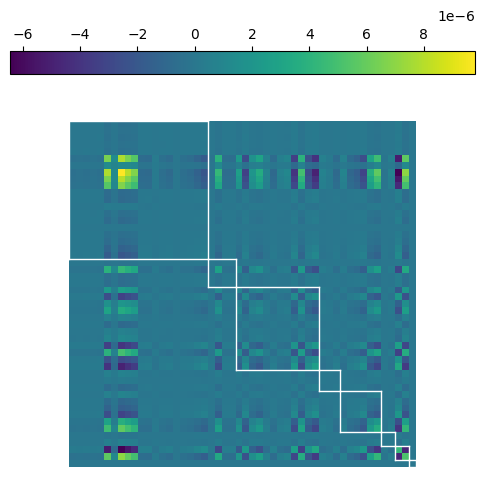
\includegraphics[width=0.43\linewidth]{kfac_pinns_exp/exp04_gramian_contributions/fig/gram_full.png}

  \begin{tabular}{ccc}
    (\textcolor{blue}{forward}, \textcolor{red}{forward})
    &
      (\textcolor{blue}{forward}, \textcolor{red}{gradient})
    &
      (\textcolor{blue}{forward}, \textcolor{red}{Hessian})
    \\
    
\includegraphics[width=0.22\linewidth]{kfac_pinns_exp/exp04_gramian_contributions/fig/gram_output_output.png}
    &
      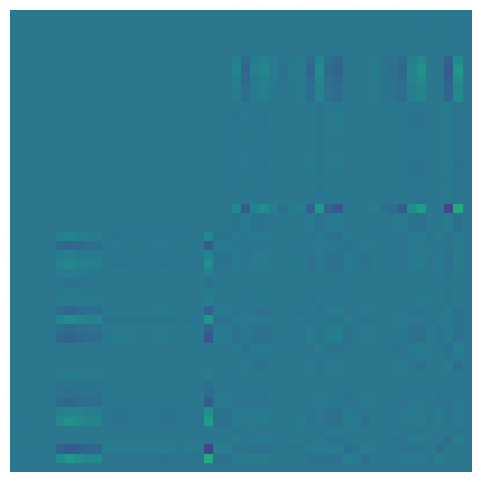
\includegraphics[width=0.22\linewidth]{kfac_pinns_exp/exp04_gramian_contributions/fig/gram_output_grad_input.png}
    &
      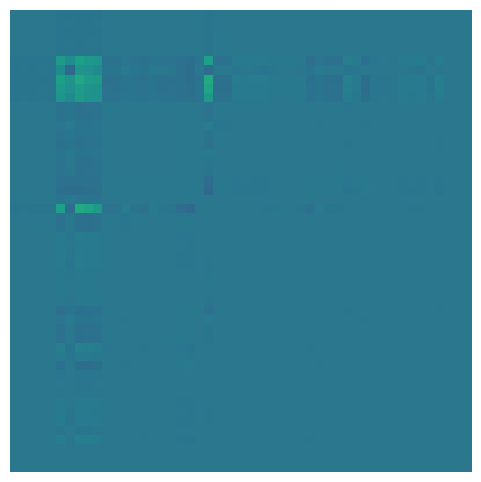
\includegraphics[width=0.22\linewidth]{kfac_pinns_exp/exp04_gramian_contributions/fig/gram_output_hess_input.png}
    \\
    (\textcolor{blue}{gradient}, \textcolor{red}{forward})
    &
      (\textcolor{blue}{gradient}, \textcolor{red}{gradient})
    &
      (\textcolor{blue}{gradient}, \textcolor{red}{Hessian})
    \\
    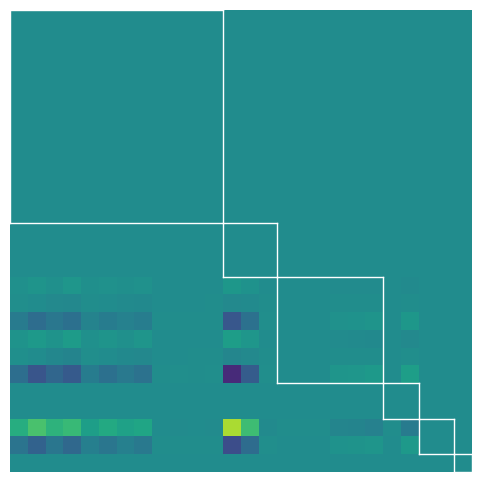
\includegraphics[width=0.22\linewidth]{kfac_pinns_exp/exp04_gramian_contributions/fig/gram_grad_input_output.png}
    &
      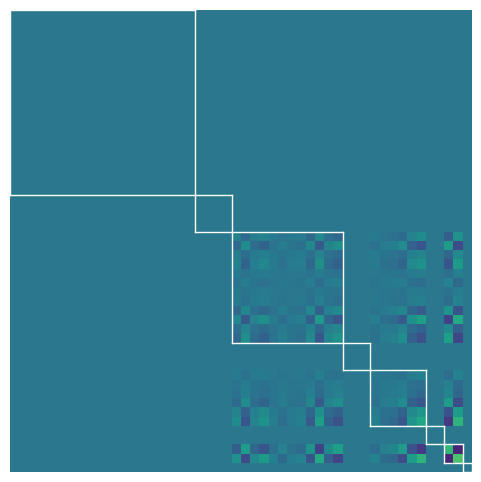
\includegraphics[width=0.22\linewidth]{kfac_pinns_exp/exp04_gramian_contributions/fig/gram_grad_input_grad_input.png}
    &
      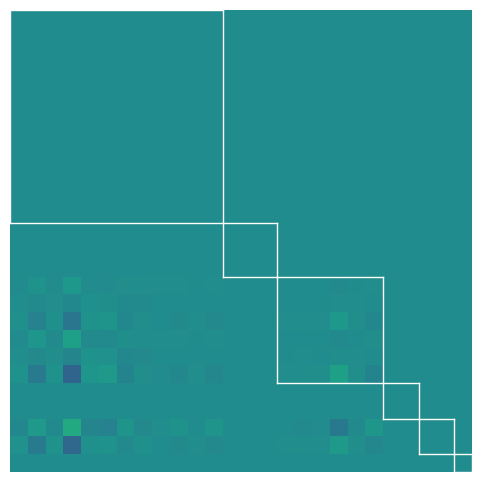
\includegraphics[width=0.22\linewidth]{kfac_pinns_exp/exp04_gramian_contributions/fig/gram_grad_input_hess_input.png}
    \\
    (\textcolor{blue}{Hessian}, \textcolor{red}{forward})
    &
      (\textcolor{blue}{Hessian}, \textcolor{red}{gradient})
    &
      (\textcolor{blue}{Hessian}, \textcolor{red}{Hessian})
    \\
    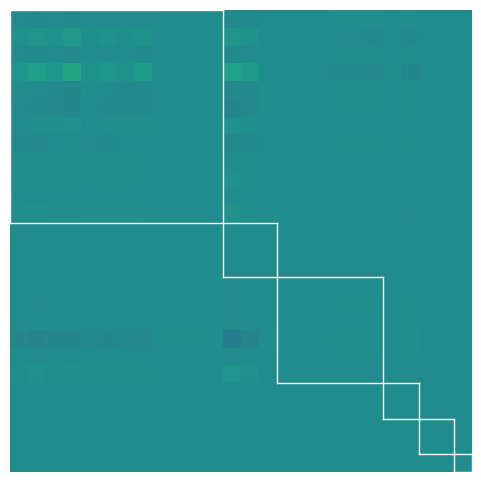
\includegraphics[width=0.22\linewidth]{kfac_pinns_exp/exp04_gramian_contributions/fig/gram_hess_input_output.png}
    &
      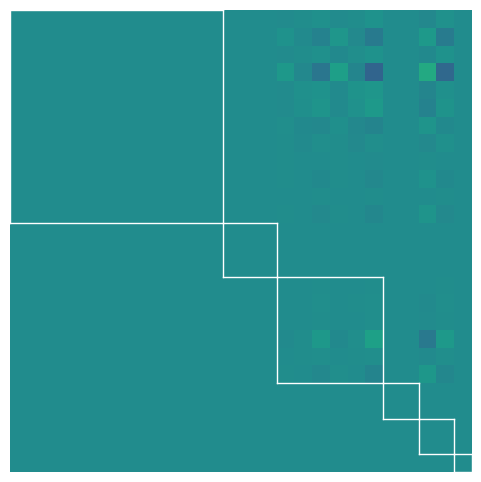
\includegraphics[width=0.22\linewidth]{kfac_pinns_exp/exp04_gramian_contributions/fig/gram_hess_input_grad_input.png}
    &
      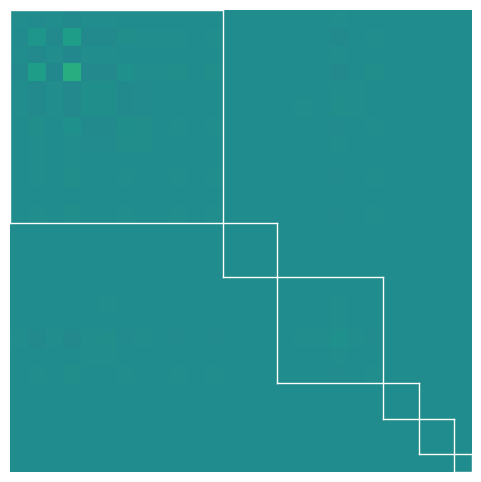
\includegraphics[width=0.22\linewidth]{kfac_pinns_exp/exp04_gramian_contributions/fig/gram_hess_input_hess_input.png}
  \end{tabular}
  \caption{Contributions $\mG_{\Omega,\textcolor{blue}{\bullet}, \textcolor{red}{\bullet}}$ to the Laplacian's Gramian $\mG_{\Omega}$ from different children in the computation graph on a synthetic toy problem.
    We use a $4 \to 3 \to 2 \to 1$ sigmoid-activated MLP and 10 randomly generated inputs. The contributions are highlighted as in \Cref{eq:fisher}.}\label{fig:gramian-contribution-children}
\end{figure}
%%% Local Variables:
%%% mode: latex
%%% TeX-master: "../main"
%%% End:


\paragraph{Computing $\jac_{\mW^{(i)}}\bullet$}
Let us first compute the Jacobians $\jac_{\mW^{(i)}}\bullet$ in \Cref{eq:laplacian-gradient}.
The Jacobian of the linear layer's forward pass is
\begin{subequations}\label{eq:fisher-jacobians}
  \begin{align}
    \jac_{\mW}\left( \mW \vx \right) = \vx^{\top} \otimes \mI\,.
  \end{align}
  The Jacobian from the gradient backpropagation is
  \begin{align}
    \jac_{\mW}\left( \mW^{\top} \vx \right) = \mI \otimes \vx^{\top}\,,
  \end{align}
  and the Jacobian from the Hessian backpropagation is
  \begin{align}\label{subeq:fisher-jacobians-hbp}
    \jac_{\mW}\left( \mW^{\top} \mX \mW \right)
    =
    \mI \otimes \mW^{\top}\mX
    +
    \mK \left(
    \mI
    \otimes
    \mW^{\top}\mX^{\top}
    \right)\,,
  \end{align}
\end{subequations}
where $\mK \in \sR^{\dim(\mZ) \times \dim(\mZ)}$ (denoting $\mZ := \mW^{\top}\mX \mW$) is a permutation matrix that, when multiplied onto a vector whose basis corresponds to that of the flattened output $\mZ$, modifies the order from first-varies-fastest to last-varies-fastest, i.e.
\begin{equation*}
  \mK \flatten(\mZ) = \flatten(\mZ^{\top})\,.
\end{equation*}
Re-introducing the layer indices, the expressions in \Cref{eq:spatialDerivatives} become
\begin{align}
  \begin{split}
    \jac_{\mW^{(i)}}\vz^{(i)}
    &=
      {\vz^{(i-1)}}^\top\otimes \mI
    \\
    \jac_{\mW^{(i)}}\grad{\vz^{(i-1)}}u\,,
    &=
      \mI\otimes
      \grad{\vz^{(i)}}u
    \\
    \jac_{\mW^{(i)}}\gradsquared{\vz^{(i-1)}}u\,,
    &=
      \mI \otimes
      \left[
      {\mW^{(i)}}^{\top}
      \left(
      \gradsquared{\vz^{(i)}}u
      \right)
      \right]
      +
      \mK
      \left(
      \mI \otimes
      \left[
      {\mW^{(i)}}^{\top}
      \left(
      \gradsquared{\vz^{(i)}}u
      \right)^{\top}
      \right]
      \right)\,.
  \end{split}
\end{align}
We will now use symmetries in the objects used during Hessian backpropagation to simplify this further.
At a first glance, it looks like the Gramian consists of 16 terms, as there are 4 summands from the Jacobians in \Cref{eq:fisher-jacobians}.
However, we can simplify into 9 terms:

First, $\gradsquared{\vz^{(i)}}u$ is symmetric, that is
\begin{align*}
  \jac_{\mW^{(i)}}\left( {\mW^{(i)}}^{\top} \left( \gradsquared{\vz^{(i)}}u  \right)\mW^{(i)} \right)
  &=
    \mI \otimes
    \left[
    {\mW^{(i)}}^{\top} \left( \gradsquared{\vz^{(i)}}u  \right)
    \right]
    +
    \mK
    \left(
    \mI \otimes
    \left[
    {\mW^{(i)}}^{\top}
    \left(
    \gradsquared{\vz^{(i)}}u
    \right)
    \right]
    \right)\,,
    \shortintertext{and the transposed Jacobian is}
  &\mI \otimes
    \left[
    \left( \gradsquared{\vz^{(i)}}u  \right) \mW^{(i)}
    \right]
    +
    \left(
    \mI \otimes
    \left[
    \left(
    \gradsquared{\vz^{(i)}}u
    \right)
    \mW^{(i)}
    \right]
    \right)
    \mK^{\top}\,.
\end{align*}
Second, we multiply the transpose Jacobian onto $\grad{\gradsquared{\vz^{(i-1)}}u}\Delta u$, which inherits symmetry from the Hessian, $[\grad{\gradsquared{\vz^{(i-1)}}u}\Delta u]_{j,k} = [\grad{\gradsquared{\vz^{(i-1)}}u}\Delta u]_{k,j}$.
Due to this symmetry, the action of $\mK$ (or $\mK^{\top}$) does not alter it,
\begin{align*}
  \mK^{\top}\left( \grad{\gradsquared{\vz^{(i-1)}}u}\Delta u \right) = \grad{\gradsquared{\vz^{(i-1)}}u}\Delta u\,.
\end{align*}
In other words, it does not matter how we flatten (first- or last-varies-fastest).
This simplifies the VJP (last line in \Cref{eq:fisher}) to
\begin{align*}
  \left(
  \mI \otimes
  \left[
  \left( \gradsquared{\vz^{(i)}}u  \right) \mW^{(i)}
  \right]
  \right)
  \grad{\gradsquared{\vz^{(i-1)}}u}\Delta u
  +
  \left(
  \mI \otimes
  \left[
  \left(
  \gradsquared{\vz^{(i)}}u
  \right)
  \mW^{(i)}
  \right]
  \right)
  \mK^{\top}
  \grad{\gradsquared{\vz^{(i-1)}}u}\Delta u
  \\
  =
  2 \left(
  \mI \otimes
  \left[
  \left( \gradsquared{\vz^{(i)}}u  \right) \mW^{(i)}
  \right]
  \right)
  \grad{\gradsquared{\vz^{(i-1)}}u}\Delta u
  \,.
\end{align*}
We can now write down the simplified Jacobian from \Cref{eq:laplacian-gradient}, whose self-outer product forms the Gramian block for a linear layer's weight matrix,
\begin{align}\label{eq:weight-jacobian-simplified}
  \begin{split}
    \jac_{\mW^{(i)}} \Delta u
    &=
      \underbrace{
      \left(
      {\vz^{(i-1)}}^\top\otimes \mI
      \right)^{\top}
      \grad{\vz^{(i)}}\Delta u
      }_{(1)}
    \\
    &\phantom{=}+
      \underbrace{
      \left(
      \mI \otimes \grad{\vz^{(i)}}u
      \right)^{\top}
      \grad{\grad{\vz^{(i-1)}}u}\Delta u
      }_{(2)}
    \\
    &\phantom{=}+
      \underbrace{
      2
      \left(
      \mI \otimes
      \left[
      \left( \gradsquared{\vz^{(i)}}u \right) \mW^{(i)}
      \right]
      \right)
      \grad{\gradsquared{\vz^{(i-1)}}u}\Delta u
      }_{(3)}
      \,,
  \end{split}
\end{align}
where (1) is the contribution from the forward pass, (2) is the contribution from the gradient backpropagation, and (3) is the contribution from the Hessian backpropagation. The Jacobians from \Cref{eq:fisher-jacobians} allow to express the Gramian in terms of Kronecker-structured expressions consisting of 9 terms in total. \Cref{fig:gramian-contribution-children} shows the 6 contributions from different children pairs.

\paragraph{Conclusion} One problem of computing the Laplacian and its Jacobian with backpropagation according to \Cref{eq:weight-jacobian-simplified} is that if we write out the Gramian's block $\mG_{\Omega}^{(i)} = \jac_{\mW^{(i)}} \Delta u (\jac_{\mW^{(i)}} \Delta u)^{\top}$, we obtain 9 terms of different structure.
Defining a single Kronecker product approximation would involve introducing new approximations on top of those employed by \citet{eschenhagen2023kroneckerfactored}.
Therefore, the forward Laplacian, or Taylor-mode, perspective we choose in the main text is advantageous as it allows to define KFAC without introducing new approximations.

\paragraph{Computing $\grad{\textcolor{blue}{\bullet}}\Delta u$}
The terms $\grad{\textcolor{blue}{\bullet}}\Delta u$ are automatically computed when computing the gradient of the loss via backdrop.

%%% Local Variables:
%%% mode: latex
%%% TeX-master: "../main"
%%% End:



%%% Local Variables:
%%% mode: latex
%%% TeX-master: "../main"
%%% End:

\newpage

\section*{NeurIPS Paper Checklist}

\begin{enumerate}
\item {\bf Claims}
\item[] Question: Do the main claims made in the abstract and introduction accurately reflect the paper's contributions and scope?
\item[] Answer: \answerYes{}
\item[] Justification: We list our contributions as bullet points in \Cref{sec:introduction} and provide references to the parts of the paper that present them.
\item[] Guidelines:
  \begin{itemize}
  \item The answer NA means that the abstract and introduction do not include the claims made in the paper.
  \item The abstract and/or introduction should clearly state the claims made, including the contributions made in the paper and important assumptions and limitations. A No or NA answer to this question will not be perceived well by the reviewers.
  \item The claims made should match theoretical and experimental results, and reflect how much the results can be expected to generalize to other settings.
  \item It is fine to include aspirational goals as motivation as long as it is clear that these goals are not attained by the paper.
  \end{itemize}

\item {\bf Limitations}
\item[] Question: Does the paper discuss the limitations of the work performed by the authors?
\item[] Answer: \answerYes{}
\item[] Justification: See the paragraph dedicated to limitations in \Cref{sec:conclusion}.
\item[] Guidelines:
  \begin{itemize}
  \item The answer NA means that the paper has no limitation while the answer No means that the paper has limitations, but those are not discussed in the paper.
  \item The authors are encouraged to create a separate "Limitations" section in their paper.
  \item The paper should point out any strong assumptions and how robust the results are to violations of these assumptions (e.g., independence assumptions, noiseless settings, model well-specification, asymptotic approximations only holding locally). The authors should reflect on how these assumptions might be violated in practice and what the implications would be.
  \item The authors should reflect on the scope of the claims made, e.g., if the approach was only tested on a few datasets or with a few runs. In general, empirical results often depend on implicit assumptions, which should be articulated.
  \item The authors should reflect on the factors that influence the performance of the approach. For example, a facial recognition algorithm may perform poorly when image resolution is low or images are taken in low lighting. Or a speech-to-text system might not be used reliably to provide closed captions for online lectures because it fails to handle technical jargon.
  \item The authors should discuss the computational efficiency of the proposed algorithms and how they scale with dataset size.
  \item If applicable, the authors should discuss possible limitations of their approach to address problems of privacy and fairness.
  \item While the authors might fear that complete honesty about limitations might be used by reviewers as grounds for rejection, a worse outcome might be that reviewers discover limitations that aren't acknowledged in the paper. The authors should use their best judgment and recognize that individual actions in favor of transparency play an important role in developing norms that preserve the integrity of the community. Reviewers will be specifically instructed to not penalize honesty concerning limitations.
  \end{itemize}

\item {\bf Theory Assumptions and Proofs}
\item[] Question: For each theoretical result, does the paper provide the full set of assumptions and a complete (and correct) proof?
\item[] Answer: \answerNA{}
\item[] Justification: Whereas we provide a derivation of the proposed Kronecker-factored approximation, our work does not provide any rigorous mathematical statements.
\item[] Guidelines:
  \begin{itemize}
  \item The answer NA means that the paper does not include theoretical results.
  \item All the theorems, formulas, and proofs in the paper should be numbered and cross-referenced.
  \item All assumptions should be clearly stated or referenced in the statement of any theorems.
  \item The proofs can either appear in the main paper or the supplemental material, but if they appear in the supplemental material, the authors are encouraged to provide a short proof sketch to provide intuition.
  \item Inversely, any informal proof provided in the core of the paper should be complemented by formal proofs provided in appendix or supplemental material.
  \item Theorems and Lemmas that the proof relies upon should be properly referenced.
  \end{itemize}

\item {\bf Experimental Result Reproducibility}
\item[] Question: Does the paper fully disclose all the information needed to reproduce the main experimental results of the paper to the extent that it affects the main claims and/or conclusions of the paper (regardless of whether the code and data are provided or not)?
\item[] Answer: \answerYes{}
\item[] Justification: We provide a detailed description of the general experimental protocol in \Cref{sec:tuning-protocol} and details for each individual experiment in~\Cref{sec:experimental_details}, including all hyper-parameter search spaces and hyper-parameters of the best runs. We also show pseudo-code for our algorithm in \Cref{app:pseudo}.
\item[] Guidelines:
  \begin{itemize}
  \item The answer NA means that the paper does not include experiments.
  \item If the paper includes experiments, a No answer to this question will not be perceived well by the reviewers: Making the paper reproducible is important, regardless of whether the code and data are provided or not.
  \item If the contribution is a dataset and/or model, the authors should describe the steps taken to make their results reproducible or verifiable.
  \item Depending on the contribution, reproducibility can be accomplished in various ways. For example, if the contribution is a novel architecture, describing the architecture fully might suffice, or if the contribution is a specific model and empirical evaluation, it may be necessary to either make it possible for others to replicate the model with the same dataset, or provide access to the model. In general. releasing code and data is often one good way to accomplish this, but reproducibility can also be provided via detailed instructions for how to replicate the results, access to a hosted model (e.g., in the case of a large language model), releasing of a model checkpoint, or other means that are appropriate to the research performed.
  \item While NeurIPS does not require releasing code, the conference does require all submissions to provide some reasonable avenue for reproducibility, which may depend on the nature of the contribution. For example
    \begin{enumerate}
    \item If the contribution is primarily a new algorithm, the paper should make it clear how to reproduce that algorithm.
    \item If the contribution is primarily a new model architecture, the paper should describe the architecture clearly and fully.
    \item If the contribution is a new model (e.g., a large language model), then there should either be a way to access this model for reproducing the results or a way to reproduce the model (e.g., with an open-source dataset or instructions for how to construct the dataset).
    \item We recognize that reproducibility may be tricky in some cases, in which case authors are welcome to describe the particular way they provide for reproducibility. In the case of closed-source models, it may be that access to the model is limited in some way (e.g., to registered users), but it should be possible for other researchers to have some path to reproducing or verifying the results.
    \end{enumerate}
  \end{itemize}


\item {\bf Open access to data and code}
\item[] Question: Does the paper provide open access to the data and code, with sufficient instructions to faithfully reproduce the main experimental results, as described in supplemental material?
\item[] Answer: \answerYes{}
\item[] Justification: We will open-source our KFAC implementations, as well as the code to fully reproduce all experiments and the original data presented in this manuscript.
\item[] Guidelines:
  \begin{itemize}
  \item The answer NA means that paper does not include experiments requiring code.
  \item Please see the NeurIPS code and data submission guidelines (\url{https://nips.cc/public/guides/CodeSubmissionPolicy}) for more details.
  \item While we encourage the release of code and data, we understand that this might not be possible, so “No” is an acceptable answer. Papers cannot be rejected simply for not including code, unless this is central to the contribution (e.g., for a new open-source benchmark).
  \item The instructions should contain the exact command and environment needed to run to reproduce the results. See the NeurIPS code and data submission guidelines (\url{https://nips.cc/public/guides/CodeSubmissionPolicy}) for more details.
  \item The authors should provide instructions on data access and preparation, including how to access the raw data, preprocessed data, intermediate data, and generated data, etc.
  \item The authors should provide scripts to reproduce all experimental results for the new proposed method and baselines. If only a subset of experiments are reproducible, they should state which ones are omitted from the script and why.
  \item At submission time, to preserve anonymity, the authors should release anonymized versions (if applicable).
  \item Providing as much information as possible in supplemental material (appended to the paper) is recommended, but including URLs to data and code is permitted.
  \end{itemize}


\item {\bf Experimental Setting/Details}
\item[] Question: Does the paper specify all the training and test details (e.g., data splits, hyperparameters, how they were chosen, type of optimizer, etc.) necessary to understand the results?
\item[] Answer: \answerYes{}
\item[] Justification: We list all details in \Cref{sec:experimental_details}.
\item[] Guidelines:
  \begin{itemize}
  \item The answer NA means that the paper does not include experiments.
  \item The experimental setting should be presented in the core of the paper to a level of detail that is necessary to appreciate the results and make sense of them.
  \item The full details can be provided either with the code, in appendix, or as supplemental material.
  \end{itemize}

\item {\bf Experiment Statistical Significance}
\item[] Question: Does the paper report error bars suitably and correctly defined or other appropriate information about the statistical significance of the experiments?
\item[] Answer: \answerYes{}
\item[] Justification: While we do not show mean and standard deviations over different model initializations for training curves, we aimed to use a thorough tuning protocol to avoid artifacts from insufficient hyper-parameter tuning and also conducted experiments with alternative hyper-parameter search methods (Bayesian versus random/grid) to ensure the consistency of our results.
\item[] Guidelines:
  \begin{itemize}
  \item The answer NA means that the paper does not include experiments.
  \item The authors should answer "Yes" if the results are accompanied by error bars, confidence intervals, or statistical significance tests, at least for the experiments that support the main claims of the paper.
  \item The factors of variability that the error bars are capturing should be clearly stated (for example, train/test split, initialization, random drawing of some parameter, or overall run with given experimental conditions).
  \item The method for calculating the error bars should be explained (closed form formula, call to a library function, bootstrap, etc.)
  \item The assumptions made should be given (e.g., Normally distributed errors).
  \item It should be clear whether the error bar is the standard deviation or the standard error of the mean.
  \item It is OK to report 1-sigma error bars, but one should state it. The authors should preferably report a 2-sigma error bar than state that they have a 96\% CI, if the hypothesis of Normality of errors is not verified.
  \item For asymmetric distributions, the authors should be careful not to show in tables or figures symmetric error bars that would yield results that are out of range (e.g. negative error rates).
  \item If error bars are reported in tables or plots, The authors should explain in the text how they were calculated and reference the corresponding figures or tables in the text.
  \end{itemize}

\item {\bf Experiments Compute Resources}
\item[] Question: For each experiment, does the paper provide sufficient information on the computer resources (type of compute workers, memory, time of execution) needed to reproduce the experiments?
\item[] Answer: \answerYes{}
\item[] Justification: We describe the hardware in \Cref{sec:experiments}.
  The total computation time can be inferred from the description of the tuning protocol in combination with the assigned time budget per run.
\item[] Guidelines:
  \begin{itemize}
  \item The answer NA means that the paper does not include experiments.
  \item The paper should indicate the type of compute workers CPU or GPU, internal cluster, or cloud provider, including relevant memory and storage.
  \item The paper should provide the amount of compute required for each of the individual experimental runs as well as estimate the total compute.
  \item The paper should disclose whether the full research project required more compute than the experiments reported in the paper (e.g., preliminary or failed experiments that didn't make it into the paper).
  \end{itemize}

\item {\bf Code Of Ethics}
\item[] Question: Does the research conducted in the paper conform, in every respect, with the NeurIPS Code of Ethics \url{https://neurips.cc/public/EthicsGuidelines}?
\item[] Answer: \answerYes{}
\item[] Justification: We have read the Code of Ethics and believe that our submission conforms to it.
\item[] Guidelines:
  \begin{itemize}
  \item The answer NA means that the authors have not reviewed the NeurIPS Code of Ethics.
  \item If the authors answer No, they should explain the special circumstances that require a deviation from the Code of Ethics.
  \item The authors should make sure to preserve anonymity (e.g., if there is a special consideration due to laws or regulations in their jurisdiction).
  \end{itemize}


\item {\bf Broader Impacts}
\item[] Question: Does the paper discuss both potential positive societal impacts and negative societal impacts of the work performed?
\item[] Answer: \answerNo{}
\item[] Justification:
  It is the goal of this paper to improve the accuracy of neural network-based PDE solvers. As the numerical solution of PDEs is a classic topic in applied mathematics and engineering, we believe there is no immediate negative societal impact.
\item[] Guidelines:
  \begin{itemize}
  \item The answer NA means that there is no societal impact of the work performed.
  \item If the authors answer NA or No, they should explain why their work has no societal impact or why the paper does not address societal impact.
  \item Examples of negative societal impacts include potential malicious or unintended uses (e.g., disinformation, generating fake profiles, surveillance), fairness considerations (e.g., deployment of technologies that could make decisions that unfairly impact specific groups), privacy considerations, and security considerations.
  \item The conference expects that many papers will be foundational research and not tied to particular applications, let alone deployments. However, if there is a direct path to any negative applications, the authors should point it out. For example, it is legitimate to point out that an improvement in the quality of generative models could be used to generate deepfakes for disinformation. On the other hand, it is not needed to point out that a generic algorithm for optimizing neural networks could enable people to train models that generate Deepfakes faster.
  \item The authors should consider possible harms that could arise when the technology is being used as intended and functioning correctly, harms that could arise when the technology is being used as intended but gives incorrect results, and harms following from (intentional or unintentional) misuse of the technology.
  \item If there are negative societal impacts, the authors could also discuss possible mitigation strategies (e.g., gated release of models, providing defenses in addition to attacks, mechanisms for monitoring misuse, mechanisms to monitor how a system learns from feedback over time, improving the efficiency and accessibility of ML).
  \end{itemize}

\item {\bf Safeguards}
\item[] Question: Does the paper describe safeguards that have been put in place for responsible release of data or models that have a high risk for misuse (e.g., pretrained language models, image generators, or scraped datasets)?
\item[] Answer: \answerNA{}
\item[] Justification: The paper does not release any data or models that have a high risk for misuse.
\item[] Guidelines:
  \begin{itemize}
  \item The answer NA means that the paper poses no such risks.
  \item Released models that have a high risk for misuse or dual-use should be released with necessary safeguards to allow for controlled use of the model, for example by requiring that users adhere to usage guidelines or restrictions to access the model or implementing safety filters.
  \item Datasets that have been scraped from the Internet could pose safety risks. The authors should describe how they avoided releasing unsafe images.
  \item We recognize that providing effective safeguards is challenging, and many papers do not require this, but we encourage authors to take this into account and make a best faith effort.
  \end{itemize}

\item {\bf Licenses for existing assets}
\item[] Question: Are the creators or original owners of assets (e.g., code, data, models), used in the paper, properly credited and are the license and terms of use explicitly mentioned and properly respected?
\item[] Answer: \answerNA{}
\item[] Justification: The paper does not use any existing assets.
\item[] Guidelines:
  \begin{itemize}
  \item The answer NA means that the paper does not use existing assets.
  \item The authors should cite the original paper that produced the code package or dataset.
  \item The authors should state which version of the asset is used and, if possible, include a URL.
  \item The name of the license (e.g., CC-BY 4.0) should be included for each asset.
  \item For scraped data from a particular source (e.g., website), the copyright and terms of service of that source should be provided.
  \item If assets are released, the license, copyright information, and terms of use in the package should be provided. For popular datasets, \url{paperswithcode.com/datasets} has curated licenses for some datasets. Their licensing guide can help determine the license of a dataset.
  \item For existing datasets that are re-packaged, both the original license and the license of the derived asset (if it has changed) should be provided.
  \item If this information is not available online, the authors are encouraged to reach out to the asset's creators.
  \end{itemize}

\item {\bf New Assets}
\item[] Question: Are new assets introduced in the paper well documented and is the documentation provided alongside the assets?
\item[] Answer: \answerNA{}
\item[] Justification: The paper does not release any new assets.
\item[] Guidelines:
  \begin{itemize}
  \item The answer NA means that the paper does not release new assets.
  \item Researchers should communicate the details of the dataset/code/model as part of their submissions via structured templates. This includes details about training, license, limitations, etc.
  \item The paper should discuss whether and how consent was obtained from people whose asset is used.
  \item At submission time, remember to anonymize your assets (if applicable). You can either create an anonymized URL or include an anonymized zip file.
  \end{itemize}

\item {\bf Crowdsourcing and Research with Human Subjects}
\item[] Question: For crowdsourcing experiments and research with human subjects, does the paper include the full text of instructions given to participants and screenshots, if applicable, as well as details about compensation (if any)?
\item[] Answer: \answerNA{}
\item[] Justification: The paper does not involve crowdsourcing nor research with human subjects.
\item[] Guidelines:
  \begin{itemize}
  \item The answer NA means that the paper does not involve crowdsourcing nor research with human subjects.
  \item Including this information in the supplemental material is fine, but if the main contribution of the paper involves human subjects, then as much detail as possible should be included in the main paper.
  \item According to the NeurIPS Code of Ethics, workers involved in data collection, curation, or other labor should be paid at least the minimum wage in the country of the data collector.
  \end{itemize}

\item {\bf Institutional Review Board (IRB) Approvals or Equivalent for Research with Human Subjects}
\item[] Question: Does the paper describe potential risks incurred by study participants, whether such risks were disclosed to the subjects, and whether Institutional Review Board (IRB) approvals (or an equivalent approval/review based on the requirements of your country or institution) were obtained?
\item[] Answer: \answerNA{}
\item[] Justification: The paper does not involve crowdsourcing nor research with human subjects.
\item[] Guidelines:
  \begin{itemize}
  \item The answer NA means that the paper does not involve crowdsourcing nor research with human subjects.
  \item Depending on the country in which research is conducted, IRB approval (or equivalent) may be required for any human subjects research. If you obtained IRB approval, you should clearly state this in the paper.
  \item We recognize that the procedures for this may vary significantly between institutions and locations, and we expect authors to adhere to the NeurIPS Code of Ethics and the guidelines for their institution.
  \item For initial submissions, do not include any information that would break anonymity (if applicable), such as the institution conducting the review.
  \end{itemize}

\end{enumerate}
%%% Local Variables:
%%% mode: latex
%%% TeX-master: "../main"
%%% End:


\end{document}
%%% Local Variables:
%%% mode: latex
%%% TeX-master: t
%%% End:
